\documentclass[toc, titlepaged]{../cs-classes/cs-classes}

\title{Introduction to Machine Learning}
\author{Alessandro Rudi, Umut \c{S}im\c{s}ekli}

\graphicspath{{../cs-classes}}

\begin{document}
\begin{abstract}
    This document is Antoine Groudiev's class notes while following the class \emph{Introduction to Machine Learning} (Apprentissage Statistique) at the Computer Science Department of ENS Ulm. It is freely inspired by the class notes written by Francis Bach, Pierre Gaillard, Alessandro Rudi, and Umut \c{S}im\c{s}ekli. 
\end{abstract}

\section{An overview of Machine Learning}
%\subsection{What is ML?}
%Considering a problem, such as image classification: given an input image of a dog or a cat, the program is asked to determine whether the image is a dog or a cat. Conventional programming would hardcode the solution to this problem. But this process takes time and is not easily generalisable. Instead, an ML model is trained on a dataset to produce a program to solve the problem.
%
%Many successfull applications of Machine Learning are:
%\begin{itemize}
%    \item Face recognition
%    \item Spam filtering
%    \item Speech recognition
%    \item Self-driving systems; pedestrian detection
%\end{itemize}
%
%\subsection{Topics in Machine Learning}
%\subsubsection{Supervised Learning}
%\begin{example}[Classification]
%    Features $x\in\R^d$, labels $y\in\{1, \dots, k\}$
%\end{example}
%
%\begin{definition}[Regression]
%    Features $x\in\R^d$, labels $y\in\R$. To tackle such problem, we look for a parametrized function $f_\theta(x_i)\simeq y_i$ for some $f_\theta$ in a function space
%    \begin{equation*}
%        \F = \{f_\theta : \theta\in\Theta\}
%    \end{equation*}
%    Our goal is therefore to find the best function in $\F$ such that $f$ "fits" the training data. For example, we can say that $f$ "fits" the training data when
%    \begin{equation*}
%        \frac{1}{n}\sum_{i=1}^n (f(x_i)-y_i)^2
%    \end{equation*}
%    is "small". Such a function is not interesting in general, like for classification. 
%\end{definition}
%
%\begin{definition}[Loss function]
%    Assums that the features are in $\mathcal{X}$ and the labels are in $\mathcal{Y}$. We introduce the more general \emph{loss function} notion:
%    \begin{equation*}
%        l:\mathcal{Y}^2\to \R_+
%    \end{equation*}
%    For a regression task, we can use $l(\hat{y}, y)=(\hat{y}-y)^2$. For a classification task, $l(\hat{y}, y)=\ind_{\hat{y}=y}$.
%\end{definition}
%
%Therefore, for a regression problem, we might choose:
%\begin{equation*}
%    f^\star=\argmin_{f\in\F}\frac{1}{n}\sum_{i=1}^n l(f(x_i), y_i)
%\end{equation*}
%In the parametric case, when $\F=\{f_\theta : \theta\in\Theta\}$, we might minimize with respect to $\theta$:
%\begin{equation*}
%    \theta^\star=\argmin_{\theta\in\Theta}\frac{1}{n}\sum_{i=1}^n l(f(x_i), y_i)
%\end{equation*}
%
%\subsubsection{Probabilistic approach}
%Let $\mathcal{Z}=\mathcal{X}\times\mathcal{Y}$ be the feature space. Let $D$ be a distribution on $\mathcal{Z}$; we make the assumption that the training data is iid from $D$:
%\begin{equation*}
%    (x_i, y_i)\sim D
%\end{equation*}
%and the same thing hold for the test data:
%\begin{equation*}
%    (\tilde{x_i}, \tilde{y_i})\sim D
%\end{equation*}
%According to the Strong Law of Large Numbers, the test loss converges almost surely:
%\begin{equation*}
%    \lim_{n\to\infty}\frac{1}{n}\sum_{i=1}^n l(f_\theta(\tilde{x_i}), \tilde{y_i}) = \E_{(x, y)\sim D}[l(f_\theta(x), y)] =: R(\theta)=R(f_\theta)
%\end{equation*}
%where $R(\theta)$ is the \emph{population risk}.
%
%\begin{definition}[Risk minimization]
%    
%\end{definition}
%
%\subsubsection{Unsupervised Learning}
%\begin{example}[Clustering]
%    
%\end{example}
%
%\begin{example}[Dimensionnality reduction]
%    We are given features $x\in \R^d$ and labels $y\in\{0, 1\}$ which form a "training" dataset $S=\{(x_1, y_1), \dots, (x_n, y_n)\}$. We assume that $d\gg1$; our goal is to find $d'\ll d$ such that $(x_1, y_1, \dots, )$
%\end{example}

\section{Linear Least Squares Regression}
%Consider an input space $X$ and an output space $Y$. We consider a function $f:X\to Y$ unknown to us, that we want to recover. We are given samples $D_N = [(x_1, y_1), \dots, (x_N, y_N)]$. Our goal is to produce $\hatf_D$ such that $\hatf_D$ "converges" to $f$ when $|D|\to+\infty$.
\subsection{Introduction}
In this chapter, we will study the simple but still widely used problem of \emph{Linear Least Square Regression}. We are given a set of points, which we assume to be sampled from some distribution: there exists some function which generated these points, and we want to retrieve or at least approximate this unknown function. To do so, we will naturally look for the function which best fits the points; nevertheless, assuming that it is unlikely that the function is overly-complicated, we will only approximate it using \emph{linear function}. Finally, to choose which linear function \say{fits best} the data, we will introduce the mean square error, which we will minimize to find our linear approximation function.

Formally, our objective is to find a function $f$ such that it explains well the distribution $(y_i)_{1\leq i\leq n}$ as a function of $(x_i)_{1\leq i\leq n}$, that is $y_i\sim f(x_i)$. To do this, we can choose a \emph{function space} $\F$ and solve the empirical risk minimization problem:
\begin{equation*}
    \hatf_n \in \argmin_{f\in\F} \hat{R}_n(f) := \argmin_{f\in\F} \frac{1}{n}\sum_{i=1}^n (y_i-f(x_i))^2
\end{equation*}
\begin{wrapfigure}[12]{l}{0.34\textwidth}
    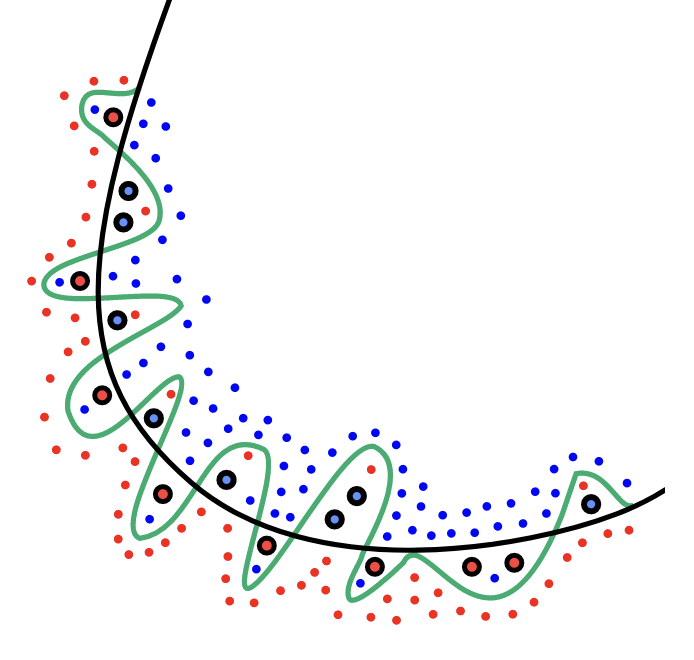
\includegraphics[width=0.3\textwidth]{images/overfitting.png}
    \caption{Example of overfitting}
\end{wrapfigure}

Care must be taken when selecting the function space to avoid overfitting\footnote{We say that the function \emph{overfits} the data when it corresponds too closely to the specific set of data (i.e.~on the training data), such that it fails to fit additional data (i.e.~test data).}: for example, if we were to choose $\F:=\R_d[X]$ for some $d\in\N$, it is in our best interest to keep $d$ small to avoid getting a function $f$ which fits perfectly the points but diverges between them. Although the empirical mean square error $\hat{R}_n$ decreases when the function space $\F$ becomes larger (i.e.~larger polynomial degrees), the $\hatf_n$ estimator loses its predictive power. $\hatf_n$ will not necessarily perform well on new data. In what follows, we will consider the linear function space, containing functions of the form $f:x\mapsto ax+b$, which is the simplest.

\subsection{General setup and notations for supervised learning}
\begin{definition}[Training data set]
    The \emph{training data set}, often denoted $D_n:=\set{(x_i, y_i)}{i\in\llbracket 1, n \rrbracket}$, is the set of some observations $(x_i, y_i)\in\X\times\Y$. We will often make the assumption that the observations $(x_i, y_i)$ are realizations of i.i.d. random variables from a distribution $\nu$.
\end{definition}

The distribution $\nu$ is unknown to the statistician; it's a matter of learning it from the data.

\begin{definition}[Learning algorithm]
    A \emph{learning algorithm} -- or \emph{learning rule} -- $\A$ is a function that associates to training data $D_n$ a prediction function $\hatf_n$:
    \begin{equation*}
        \begin{aligned}
            \A: \bigcup_{n\in\N} (\X\times\Y)^n &\longrightarrow \Y^\X\\
            D_n &\longmapsto \hatf_n
        \end{aligned}
    \end{equation*}
    The estimated function $\hatf_n$ is constructed to predict a new output $y$ from a new input $x$, where $(x, y)$ is a pair of \emph{test data}, i.e.~not necessarily observed in the training data. The function $\hatf_n$ is an estimator because it depends on the data $D_n$ and not on unobserved parameter, such as the distribution $\nu$. If $D_n$ is random, it is also a random function.
\end{definition}

\begin{definition}[Squared Loss Risk]
    Given an estimator $\hatf_n$, we define its risk:
    \begin{equation}
        \label{eq:sq-risk}
        \risk(\hatf_n) := \E\left[(Y-\hatf_n(X))^2\,\big| \, D_n\right] \where (X, Y)\sim\nu
    \end{equation}
    This is also called the \emph{generalization error}, as it measures how well the estimator performs on other inputs and outputs of the dataset.
\end{definition}

In practice, the statistician cannot compute the risk, since one cannot acces the distribution $\nu$. Therefore, a common method in supervised machine learning is to replace the risk (defined using the distribution $\nu$ through the expectation $\E$) by the empirical risk (defined using the training data set).

\begin{definition}[Squared Loss Empirical risk]
    Given an estimator $\hatf_n$ and a data set $D_n=\set{(x_i, y_i)}{i\in\iset{1}{n}}$, we define its \emph{empirical risk}:
    \begin{equation}
        \label{eq:sq-empirical-risk}
        \emrisk_n(\hatf_n) := \frac{1}{n}\sum_{i=1}^n (y_i-\hatf_n(x_i))^2
    \end{equation}
\end{definition}

\begin{wrapfigure}[15]{r}{0.45\textwidth}
    \centering
    \captionsetup{justification=centering}
    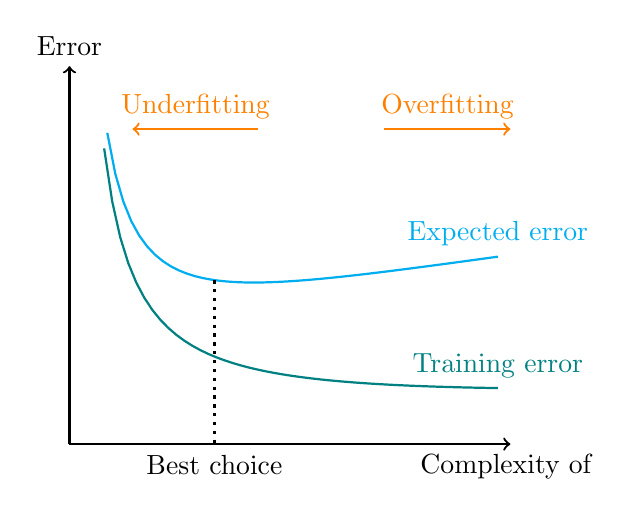
\begin{tikzpicture}[scale=0.8]
        \draw[domain=0.55:6.8, samples=50, color=teal, thick] plot (\x, 2.5/\x + 0.2*\x^0.5) node[above] {Training error};
        \draw[domain=0.6:6.8, samples=50, color=cyan, thick] plot (\x, 2.5/\x + 1*\x^0.5) node[above] {Expected error};
        \draw[dotted, very thick] (2.3, 2.6) -- (2.3, 0) node[below] {Best choice};
        \draw[->, thick] (0,0) -- (7,0) node[below] {Complexity of $\F$};
        \draw[->, thick] (0,0) -- (0,6) node[above] {Error};

        \draw[->, color=orange, thick] (5, 5) -- (7, 5) node[above, pos=0.5] {Overfitting};
        \draw[->, color=orange, thick] (3, 5) -- (1, 5) node[above, pos=0.5] {Underfitting};
      \end{tikzpicture}
    \caption{Overfitting and underfitting}
\end{wrapfigure}
However, one must be careful about overfitting, the case where $\emrisk_n(f)$ is much lower than $\risk(f)$, as discussed previously. In this chapter, we will study the performance of the least square estimator in the case of the linear model.

\begin{definition}[Linear model]
    When $\X=\R^d$ and $\Y=\R$, the simplest interesting function space is the set of affine functions. To ease the notation, we assume that the frist components of the inputs is 1 so that it is sufficient to consider linear functions. Therefore, the function space is:
    \begin{equation}
        \F:=\set{x\mapsto \theta^\tp x}{\theta\in\R^d}
    \end{equation}
    i.e.~linear functions parametrized by $\theta\in\R^d$.
\end{definition}

\begin{remark}
    Choosing a linear model, the empirical risk minimization corresponds to the problem of minimizing the following quantity over $\theta\in\R^d$:
    \begin{equation*}
        \emrisk_n(\theta):=\frac{1}{n}\sum_{i=1}^n(y_i-\theta^\tp x_i)^2
    \end{equation*}
    This expression can be rewritten using matrix notation. We let $Y=(Y_1, \dots, Y_n)^\tp\in\R^n$ be the vector of outputs and $X\in\R^{n\times d}$ the matrix of inputs, whose rows are $x_i^\tp$. $X$ is called the \emph{design matrix}. The empirical risk is therefore given by:
    \begin{equation*}
        \emrisk_n(\theta)=\frac{1}{n}\norm{Y-X\theta}^2_2
    \end{equation*}
\end{remark}

\subsection{Ordinary Least Squares Estimator (OLS)}
\subsubsection{Definition and closed form}
In the following, we assume that the design matrix is injective.\footnote{Said otherwise, the rank of $X$ is $d$.} In particular, $d\leq n$, otherwise this is not possible.

\begin{definition}[Ordinary Least Squares]
    If $X$ is injective, the minimizer of the empirical risk \eqref{eq:sq-empirical-risk} is called the \emph{Ordinary Least Squares (OLS) estimator}. Said otherwise, it is the vector $\htheta\in\R^d$ minimizing $\emrisk_n$:
    \begin{equation}
        \label{eq:ols-estimator}
        \htheta := \argmin_{\theta\in\R^d} \emrisk_n(\theta)=\argmin_{\theta\in\R^d}\frac{1}{n}\sum_{i=1}^n(y_i-\theta^\tp x_i)^2
    \end{equation}
\end{definition}

\begin{property}[Closed form soluion of the OLS estimator]
    \label{prop:closed-form-OLS}
    If $X$ is injective, the OLS estimator exists and is unique. Moreover, it is given by:
    \begin{equation}
        \label{eq:closed-form-OLS}
        \htheta = (X^\tp X)^{-1}X^\tp Y
    \end{equation}
\end{property}

\begin{proof}
    Since $\emrisk_n$ is coercive\footnote{$\norm{\emrisk_n(\theta)} \xrightarrow[\norm{\theta}\to+\infty]{} +\infty$} and continuous, it admits at least a minimizer. Furthermore, we have:
    \begin{equation*}
        \emrisk_n(\theta) := \frac{1}{n}\norm{Y-X\theta}^2_2 = \frac{1}{n}\left(\theta^\tp(X^\tp X)\theta - 2\theta^\tp X^\theta Y+\norm{Y}^2\right)
    \end{equation*}
    Since $\emrisk$ is differentialble any mimizer cancels its gradient:
    \begin{equation*}
        \nabla\emrisk_n(\htheta) = \frac{1}{n}\left(\htheta^\tp(X^\tp X) + (X^\tp X)\htheta - 2X^\tp Y\right) = \frac{2}{n}\left((X^\tp X)\htheta - Y^\tp X\right)
    \end{equation*}
    where the last equality holds because $X^\tp X\in\R^{d\times d}$ is symmetric. Since $X$ is injective, $X^\tp X$ is invertible\footnote{It is even positive definite.}. Therefore, a solution of $\nabla\emrisk_n(\htheta)=0$ satisfies:
    \begin{equation*}
        \htheta = (X^\tp X)^{-1}XY
    \end{equation*}
    Finally, this unique solution is indeed a minimum since its Hessian is definite positive:
    \begin{equation*}
        \nabla^2\emrisk_n(\htheta) = \frac{2}{n}(X^\tp X)
    \end{equation*}
\end{proof}

\subsubsection{Geometric interpretation}
The linear model aims modeling the ouput vector $Y\in\R^n$ by a linear combination of the form $X\theta\in\R^n$. The image of $X$ is the solution space, denoted:
\begin{equation*}
    \im(X)=\set{X\theta\in\R^n}{\theta\in\R^d}
\end{equation*}
This is the vector subspace of $\R^n$ generated by the $d\leq n$ columns of the design matrix. As $\rg(X)=d$, it is of dimension $d$.

By minimizing $\norm{Y-X\theta}$, we thus look for the element of $\im(X)$ closest to $Y$. This is the orthogonal projection of $Y$ on $\im(X)$, denoted $\hat{Y}$. By definition of the OLS and by Property \ref{prop:closed-form-OLS}, we have:
\begin{equation*}
    \hat{Y} := X\htheta = X(X^\tp X)^{-1}X^\tp Y
\end{equation*}
In particular, $P_X:=X(X^\tp X)^{-1}X^\tp$ is the projection matrix on $\im(X)$.

\subsubsection{Numerical resolution}
The closed form formula \eqref{eq:closed-form-OLS} of the OLS is useful in analyzing it; however, calculating it naively can be prohibitively expensive. For example, when $d$ is large, one prefers to avoid inverting the design matrix $X^\tp X$ which costs $O(d^3)$\footnote{Using the Gauss-Jordan method}, and can be very unstable when the matrix is badly conditioned. The following methods are usually preferred.

\paragraph*{QR factorization}
To improve stability, $QR$ decomposition can be used. Since $\htheta$ is the solution of the equation:
\begin{equation*}
    (X^\tp X)\htheta = X^\tp Y
\end{equation*}
we write $X\in\R^{n\times d}$ as $X=QR$ where $Q\in\R^{n\times d}$ is an orthogonal matrix\footnote{That is $QQ^\tp=I_n$} and $R\in\R^{d\times d}$ is upper triangular. Upper triangular matrices are very useful for solving linear systems. Substituting in the previous equation, we get:
\begin{equation*}
    \begin{aligned}
        R^\tp(Q^\tp Q)R\htheta = R^\tp Q^\tp Y &\iff R^\tp R\htheta = R^\tp Q^\tp Y \\
        &\impliedby R\htheta = Q^\tp Y
    \end{aligned}
\end{equation*}
All that remains is to solve a linear system with a triangular upper matrix, which is easy.

\begin{wrapfigure}[11]{l}{0.5\textwidth}
    \centering
    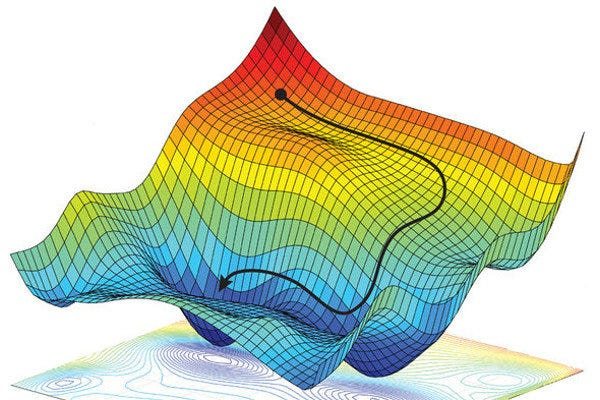
\includegraphics[width=0.4\textwidth]{images/gradient-descent.jpg}
    \caption{(Non-convex) Gradient descent}
\end{wrapfigure}
\paragraph*{Gradient descent}
We can completely bypass the need of matrix inversion or factorization using gradient descent. It consists in solving the minimization problem step by step by approching the minimum throught gradient steps. For example, we initialize $\theta_0:=0$\footnote{In practice, $\theta_0$ is often initialized to some random vector to avoid singularities.}, then update it using the following recurrence formula:
\begin{equation*}
    \begin{aligned}
        \theta_{i+1} :=&\, \theta_i -\eta\cdot\nabla\emrisk_n(\theta_i)\\
        =&\, \theta_i - \eta\cdot\frac{2}{n}\left((X^\tp X)\theta_i - Y^\tp X\right)
    \end{aligned}
\end{equation*}
where $\eta>0$ is a learning parameter called \emph{learning rate}. We see that if the algorithm converges, then it converges to a point cancelling the gradient, thus to the (unique) OLS solution. For the algorithm to converge, the learning rate $\eta$ must be well calibrated. This will be seen in more details in the following chapter about gradient descent.

If the data set is too big, i.e.~when $n\gg1$, loading all the data to make the gradient calculation $\nabla\emrisk(\theta_i)$ can be prohibitively expensive too. The common solution to this is to use \emph{Stochastic Gradient Descent}, where gradient calculations for one step are made only on estimates of $\nabla\emrisk(\theta_i)$, calculated on a random subset of the data.

\subsubsection{Nonlinear problem: polynomial, spline, and kernel regression}
The assumption tha the observations $y_i$ can be explained as a linear combination of the explanatory variables $x_{i, j}$ may seem strong. However, the previous linear framework can be applied to transformations of the variables $x_{i, j}$. For example, by adding the powers of the variables $x^k_{i, j}$ or their products $x_{i, j}\cdot x_{i', j'}$, this allows comparison to polynomial spaces. Doing a linear regression on polynomial transformations of variables is equivalent to doing a polynomial regression.

Of course, other bases and transformations exist: for instance, \emph{spline bases} are piecewise polynomials with constraints on the edgets. This is the model used for example by EDF to predict electricity consumption as a function of variables such as the time of the day, the day of the week, temperature or cloud cover.
In general, we can consider transformations $\varphi:\X\to\R^d$ and try to explain the outputs $y_i$ with functions of the form $\theta\to\varphi(x_i)^\tp \theta$. Another form of regression that we will discuss in the following is therefore \emph{kernel regression}, which allows computing efficiently the estimator even when $\varphi$ maps to an infinite dimensional space.

\subsection{Statistical analysis}
In this section, we try to show some guarantees for the OLS estimator, such as a bound the excess risk of the OLS, which we will define later on.
\subsubsection{Stochastic assumptions and bias/variance decomposition}
To provide guarantees on the performance of OLS, we require assumptions about how the data is generated. In this section, we consider a stochastic framework that will allow us to statistically analyze OLS.

\paragraph*{Assumption: linear model}
We assume that there exists a vector $\theta^*\in\R^d$ such that for all $1\leq i\leq n$, 
\begin{equation}
    \label{eq:assumption-linear-model}
    Y_i = x_i^\tp \theta^* + Z_i
\end{equation}
where $Z=(Z_1, \dots, Z_n)^\tp\in\R^n$ is a vector of \emph{errors}, also called \emph{noise}. The $Z_i$ are assumed to be centered independent variables of variance $\sigma^2$, i.e. $\E[Z_i]=0$ and $\V[Z_i]=\sigma^2$. The assumption \eqref{eq:assumption-linear-model} can be rewritten in matrix form:
\begin{equation}
    Y=X\theta^*+Z
\end{equation}
where $Y=(Y_1, \dots, Y_n)^\tp\in\R^n$, $X=(x_1, \dots, x_n)^\tp\in\R^{n\times d}$, and $Z=(Z_1, \dots, Z_n)^\tp\in\R^n$.

\begin{remark}
    We write $Y_i$ and $Z_i$ using capital letters to remind ourselves that they are random variables. The noise $Z$ comes from the fact that in practice, the observations $Y_i$ never completely fit the linear forecast. They are due to noise or unobserved explanatory variables. As before, we assume that the first vector of the explanatory variable is the constant vector, i.e. $\forall i, x_{i, 1}=1$
\end{remark}

\paragraph*{Analysis settings}
Two settings of analysis can be chosen:
\begin{itemize}
    \item In the \emph{fixed desing} setting, the design matrix $X$ is not random but deterministic and the features $x_1, \dots, x_n$ are fixed. The expectations are thus only with respect to the $Z_i$ and the $Y_i$, and the goal is to minimize:
    \begin{equation*}
        \risk_X(\theta) = \E\left[\frac{1}{n}\sum_{i=1}^n (Y_i-x_i^\tp\theta)^2\right]
    \end{equation*}
    for new random observations $Y_i$, but on the same inputs.
    \item In the \emph{random design} setting, both the inputs and the ouputs are random. This is the most standard setting in supervised machine learning. The goal is therefore to minimize the risk \eqref{eq:sq-risk} -- also called the generalization error.
\end{itemize}
In this chapter, we will consider the fixed design setting, because it eases both the notation and the calculations -- we will only need some simple linear algebra.

Before analyzing the statistical properties of OLS, we state a general result under the linear model assumption, which illustrates the tradeoff between estimation and approximation -- or bias and variance.

\begin{property}[Risk decomposition]
    Under the linear model assumption with fixed design, the following hols:
    \begin{equation*}
        \forall \theta\in\R^d, \quad \E[\risk_X(\theta)-\risk_X(\theta^*)] = \norm{\theta-\theta^*}^2_\Sigma
    \end{equation*}
    where $\Sigma:=\frac{1}{n}X^\tp X\in\R^{d\times d}$ and $\norm{\alpha}^2_\Sigma:=\alpha^\tp\Sigma\alpha$. Furthermore, if $\theta$ is a random variable -- when it depends on a random dataset -- we have:
    \begin{equation*}
        \E[\risk_X(\theta)]-\risk(\theta^*) = \underbrace{\norm{\E[\theta]-\theta^*}^2_\Sigma}_{\textnormal{Bias}} + \underbrace{\E\left[\norm{\theta-\E[\theta]}^2_\Sigma\right]}_{\textnormal{Variance}}
    \end{equation*}
\end{property}
\begin{proof}
    %TODO
\end{proof}

\begin{remark}
    It is worth to note that the optimal risk satisfies:
    \begin{equation*}
        \risk_X(\theta^*) = \E\left[\frac{1}{n}\sum_{i=1}^n(Y_i-x_i^\top\theta^*)^2\right] = \E\left[\frac{1}{n}\sum_{i=1}^nZ_i^2\right] = \frac{1}{n}\sum_{i=1}^n\E[Z_i^2]=\sigma^2
    \end{equation*}
\end{remark}

\subsubsection{Statistical properties of OLS}
We can now show some guarantees for the OLS estimator.

\begin{property}
    Under the linear model assumption with fixed design, the OLS estimator $\htheta$ defined by \eqref{eq:ols-estimator} satisfies:
    \begin{equation*}
        \E[\htheta] = \theta^* \quad \textnormal{and} \quad \V[\htheta] = \frac{\sigma^2}{n}\Sigma^{-1}
    \end{equation*}
    i.e. it is unbiased, and its variance is some $O(n^{-1})$. Furthermore, we can even show that it satisfies the Gauss-Markov property: it is optimal among all unbiased estimators of $\theta$, in the sense that is has a minimal variance-covariance matrix.
\end{property}

\begin{proof}
    %TODO
\end{proof}

\begin{definition}[Excess risk]
    The excess risk of an estimator $\htheta$ is defined by:
    \begin{equation}
        \label{eq:excess-risk}
        \exrisk(\htheta) := \E[R_X(\htheta)]-\risk(\theta^*)
    \end{equation}
    It allows to measure the risk induced by the use of an estimator instead of the optimal vector, without taking into account the inherent risk generated by the noise, which cannot be reduced.
\end{definition}

\begin{corollary}[Excess risk of OLS]
    Under the linear model assumption with fixed design, the excess risk of the OLS satisfies:
    \begin{equation*}
        \exrisk(\htheta) := \E[\risk_X(\htheta)]-\risk(\theta^*)=\frac{\sigma^2d}{n}
    \end{equation*}
\end{corollary}

\begin{proof}
    % TODO
\end{proof}

\subsubsection{Gaussian noise model}
A special case that is often considered is Gaussian noise, i.e. $Z_i\sim\mathcal{N}(0, \sigma^2)$, the normal distribution of expectation 0 and variance $\sigma^2$. This choice comes not only from the fact that it allows to compute many additional statistical properties on $\htheta$ and to perform tests, such as confidence intervals or significance of variables. In practice, it is also motivated by the central limit theorem, and the fact that noise is often an addition of many phonomena not explained by the linear combination of the explanatory variables.

\begin{property}
    In the linear model with Gaussian noise, the maximum likelihood estimators of $\theta$ and $\sigma$ satisfy respectively:
    \begin{equation*}
        \htheta_{MV}=(X^\tp X)^{-1}XY \quad \textnormal{and} \quad \hat{\sigma}^2_{MV}=\frac{\norm{Y-X\htheta}^2}{n}
    \end{equation*}
    We therefore find the least squares estimator obtained by minimizing the empirical risk. The variance estimator is biased. We will see more about maximum likelihood estimators in next chapters.
\end{property}

\subsection{Ridge regression}
\subsubsection{Handling non-injective design matrices}
If $X$ is not injective, the matrix $X^\tp X$ is no longer invertible and the OLS optimization problem admits several solutions. The problem is said to be \emph{poorly posed} or \emph{unindentifiable}. Since the variance of $\htheta$ depends on the conditioning of the matrix $(X^\tp X)^{-1}$, the more columns of it are likely to be dependent, the less stable $\htheta$ will be. Several solutions allow dealing with the case where $\rg(X)<D$.

\emph{Explicit complexity control} reduces the $\im(X)$ solution space: this can be done by removing columns from the $X$ matrix until it becomes injective (for example, by reducing the degree of polynomials). One can also set identifiability constraints of the form $\theta\in V$, a vector subspace of $\R^d$ such that any element $y\in\im(X)$ has a unique antecedent $\theta\in V$ with $y=X\theta$. For example, we could choose $V=\ker(X)^\bot$.

\emph{Implicit complexity control} regularizes the empirical risk minimization problem. The most common approach is to regularize by adding $\norm{\theta}^2_2$ (Ridge regression) or $\norm{\theta}_1$ (Lasso regression).

\subsubsection{Ridge regression}
\begin{definition}
    For a regularization parameter $\lambda$, the Ridge regression estimator is defined as
    \begin{equation}
        \htheta_\lambda \in \argmin\set{\frac{1}{n}\norm{Y-X\theta}^2_2+\lambda\norm{\theta}^2_2}{\theta\in\R^d}
    \end{equation}
    The regularization parameter $\lambda>0$ regulates the trade-off between the variance of $\htheta$ and its bias.
\end{definition}

\begin{property}
    The Ridge regression estimator is unique and satisfies:
    \begin{equation*}
        \htheta_\lambda = (X^\tp X+n\lambda I_n)^{-1}X^\tp Y
    \end{equation*}
\end{property}
\begin{proof}
    Similar to the one of the OLS and left as an exercise. We can see that there is no longer the problem of inverting $X\tp X$ since the Ridge regression replaces $(X^\tp X)^{-1}$ by $(X^\tp X+n\lambda I_n)^{-1}$ in the OLS solution.
\end{proof}

\begin{property}[Risk of Ridge regression]
    Under the linear model assumption, the Ridge regression estimator satisfies:
    \begin{equation*}
        \E[\risk_X(\htheta_\lambda)]-\risk_X(\theta^*) = \sum_{j=1}^d(\theta_j^*)^2\frac{\lambda_j}{(1+\lambda_j/\lambda)^2} + \frac{\sigma^2}{n}\sum_{j=1}^d\frac{\lambda_j^2}{(\lambda_j+\lambda)^2}
    \end{equation*}
    where $\lambda_j$ is the $j$-th eigenvalue of $\Sigma=\frac{1}{n}X^\tp X$. In particular, the choice of:
    \begin{equation*}
        \lambda^* = \frac{\sigma\sqrt{\Tr(\Sigma)}}{\norm{\theta^*}_2\sqrt{n}}
    \end{equation*}
    yiels the following excess risk:
    \begin{equation*}
        \E[\risk_X(\htheta_{\lambda^*})]-\risk_X(\theta^*) \leq \frac{\sigma\sqrt{2\Tr(\Sigma)\norm{\theta^*}_2}}{\sqrt{n}}
    \end{equation*}
\end{property}
\begin{proof}
    Follows from the bias-variance decomposition, and is left as an exercise.
\end{proof}

\begin{remark}
    As $\lambda\to0$, its excess risk converges to the one of OLS. The first term corresponds to the bias of the Ridge estimator. Thus, on the downside, the Ridge estimator is biased in constrast to the OLS. But on the positive side, its variance does not involve the inverse of $\Sigma$ but of $\Sigma+\lambda I_d$ instead, which is better conditioned. It has therefore a lower variance. The parameter $\lambda$ controls the trade-off.
\end{remark}

\subsubsection{Comparaison to the OLS}
We can compare the excess risk bound obtained by $\htheta_{\lambda^*}$ with the one of the OLS, which was $\sigma^2d/n$.
\begin{itemize}
    \item The OLS convergence is in $O(n^{-1})$ while the convergence of $O(n^{-1/2})$, which is slower
    \item The OLS dependency on the noise is in $\sigma^2$ while Ridge's is in $\sigma$, which is better
    \item Since $\Tr(\Sigma)\leq\max_{1\leq i\leq n}\norm{x_i}^2$, if the input norms are bounded by $R$, the excess risk of Ridge does not depend on the dimension $d$, which can even be infinite. It is called a \emph{dimension free} bound.
\end{itemize}
The calibration of the regularization parameter is therefore essential in practice. It can for example be done analytically as in the proposition -- but often, some quantities such as $\sigma^2$ and $\norm{\theta^*}$ are unknown. In practice, one resorts to train/validation set or \emph{cross-validation}.

\section{Logistic regression and convex analysis}
%\subsection*{Recap of important notions and notations}
%We are given an input space $X$ and an output space $Y$. We want to learn the relationship between input and output, modelised by a probability distribution $\rho\in \P(X\times Y)$. Thus, we try to find the best function $f_\star:X\to Y$, given a loss function $l:Y\times Y\to\R$. Therefore, $f_\star$ is often defined by:
%\begin{equation*}
%    f_\star = \argmin_{f:X\to Y} \E_{X, Y}[l(f(X), Y)]
%\end{equation*}
%where
%\begin{equation*}
%    \E_{X, Y}[g(X, Y)] = \int_{\R^2} g(x, y) \cdot \mathrm{d}\rho(x, y)
%\end{equation*}
%
%In practice, you only know some samples $D_N=[(x_1, y_1), \dots, (x_N, y_N)]$ with $(x_i, y_i) \sim \rho$, making it impossible to choose such an $f_\star$. Therefore, we try to find a good model $\hatf_{D_N}$, such that
%\begin{equation*}
%    \lim_{N\to+\infty}\mathcal{E}(\hatf_{D_N}) - \mathcal{E}(f) = 0
%\end{equation*}
%Such a result will often be given by a \emph{learning rate function} $c(N)$, with
%\begin{equation*}
%    \E_{D_N}[\mathcal{E}(\hatf_{D_N}) - \mathcal{E}(f)] \leq c(N) = o(1)
%\end{equation*}
%The function $\hatf_{D_N}$ can be chosen such that it minimizes the empirical error:
%\begin{equation*}
%    \hatf_{D_N} = \argmin_{f\in\mathcal{H}}\hat{\mathcal{E}}(f) = \argmin_{f\in\mathcal{H}} \frac{1}{N} \sum_{i=1}^N l(f(x_i), y_i)
%\end{equation*}
%
%\subsection{}
%We consider the case where $X=\R^d$ and $Y=\R$. We define the loss $l$ to be the least squares, $l(y, y') = (y-y')^2$, and we choose our functions to be of the form of $f_\star = \theta_\star^T X$. In this case, ERM is OLS:
%\begin{equation*}
%    \htheta_N = \argmin_{\theta\in\R^d} \frac{1}{N} \sum_{i=1}^N (\theta^Tx_i-y_i)^2
%\end{equation*}
%
%We can also define $\htheta_{N, \lambda}$ to be:
%\begin{equation*}
%    \htheta_{N, \lambda} = \argmin_{\theta\in\R^d} \frac{1}{N} \sum_{i=1}^N (\theta^Tx_i-y_i)^2 + \lambda\norm{\theta}^2
%\end{equation*}
%This allows to regulate the "complexity" of the function to avoid overfitting. This is called Tikhonov regularization. In this case, we have
%\begin{equation*}
%    \E_{\hat{Y}}[\mathcal{\htheta_N} - \mathcal{E}(\theta_\star)] = \frac{\sigma^2 d}{N}
%\end{equation*}
%and therefore the optimal function is 
%\begin{equation*}
%    \hatf_{N, \lambda} = \argmin_{f\in\mathcal{H}} \hat{\mathcal{E}}(f) + \lambda R(f)
%\end{equation*}
%
%We define $X\in\R^{N\times d} := (x_1^T, \dots, x_N^T)$, and $\hat{Y}=(\hat{y}_1, \dots, \hat{y}_n)$. We this notation, we have
%\begin{equation*}
%    \htheta_{N, \lambda} = \frac{1}{N}||X\theta-\hat{Y}||^2 + \lambda||\theta||^2
%\end{equation*}
%Thus, we have
%\begin{equation*}
%    \begin{aligned}
%        \nabla\mathcal{L}(\theta) := \frac{2}{N}X^TX\theta - 2\frac{X^T\hat{Y}}{N}+2\lambda\theta &= 0\\
%        (\frac{X^TX}{N}+\lambda)\theta &= X^T\hat{Y}
%    \end{aligned}
%\end{equation*}
%therefore,
%\begin{equation*}
%    \htheta_{N, \lambda} = \left(\frac{X^TX}{N}+\lambda I\right)^{-1}\frac{X^T\hat{Y}}{N} = \left(X^TX+\lambda N I\right)^{-1}X^T\hat{Y}
%\end{equation*}
%We introduce the singular value decomposition of $X$:
%\begin{equation*}
%    X = U\Sigma V^T
%\end{equation*}
%where $U^TU = UU^T = I_N$, $V^TV = VV^T=I_d$, and $\Sigma$ is diagonal with $\forall i, \,\Sigma_{i, i} \geq 0$.
%In this case,
%\begin{equation*}
%\begin{aligned}
%    X^TX + \lambda NI_d &= V\Sigma U^T U \Sigma V^T + \lambda N I_d\\
%    &= V(\underbrace{\Sigma^2 + \lambda N I}_{\textnormal{invertible}}) V^T
%\end{aligned}
%\end{equation*}

This chapter will introduce logistic regression, a widely used classification algorithm. Unlike linear regression, there is no closed-form solution and one needs to solve it using iterative convex optimization algorithms.

\subsection{Logistic regression}
We consider the binary classification problem: given inputs in $\R^d$, we want to predict outputs in $\{0, 1\}$. We are given a training set $D_n=\set{(X_i, Y_i)}{i\in\iset{1}{n}}$, where the data points $(X_i, Y_i)$ are i.i.d. random variables following a distribution $\nu$ in $\X\times\Y=\R^d\times\{0, 1\}$

\subsubsection{Motivation}
We would like to use an algorithm similar to linear regression introduced in the previous chapter. However, since the outputs $Y_i$ are binary and belong to $\{0, 1\}$, a discrete set, we cannot predict them using a linear transformation of the inputs $X_i$. We will thus classify the data based on a classification rule of the form
\begin{equation*}
    f : \R^d \longrightarrow \R
\end{equation*}
which will then be passed through a function with specification $\R\to\{0, 1\}$. The final estimator will therefore be:
\begin{equation*}
    \ind_{\R_+}\circ f
\end{equation*}
meaning that the estimator will predict $Y_i=+1$ exactly when $f(X_i)\geq0$.

More precisely, we will consider linear functions $f$ of the form:
\begin{equation*}
    f_\beta = x \longmapsto x^\tp\beta
\end{equation*}
This assumes that the data is \emph{linearly separable}, meaning that it can be well-explained by a linear separation.
\begin{figure}[H]
    \centering
    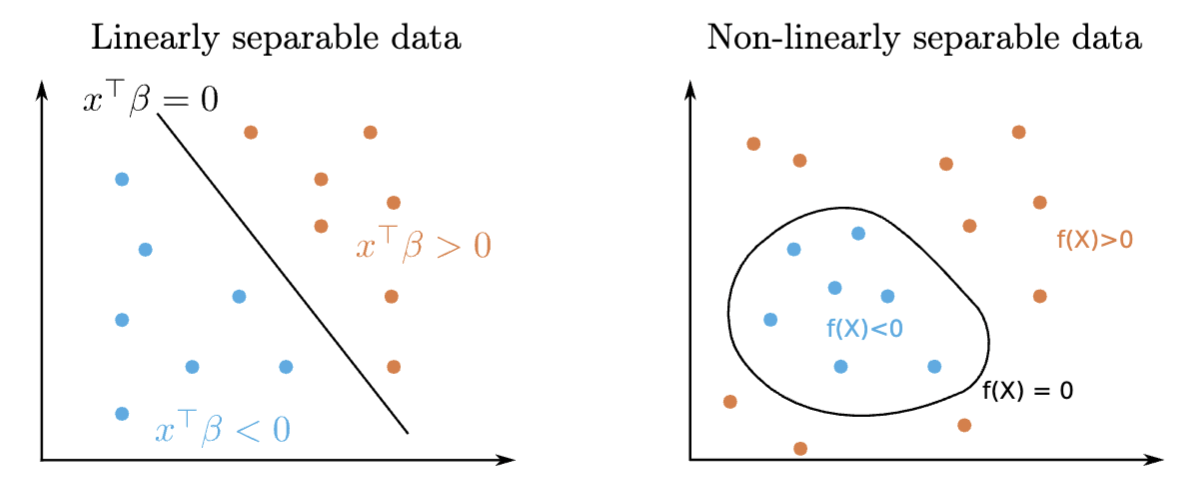
\includegraphics[width=0.8\textwidth]{images/linearly-separable.png}
    \caption{Data that can or cannot be well-explained by a linear separation}
\end{figure}
If the data does not seem to be linearly separable, we can use similar tricks as the one introduced for linear regression (polynomial regression, kernel regression, splines, \dots). We will dive into more details in an upcoming chapter about kernels.

\subsubsection{Loss function}
To minimize the empirical risk, it remains to choose a loss function to assess the performance of a prediction. 

\begin{definition}[Loss function]
    A \emph{loss function} $\ell$ is a function of the form
    \begin{equation*}
        \ell : \Y\times\Y' \longrightarrow \R_+
    \end{equation*}
    such that for $(y, y')\in\Y\times\Y'$, $\ell(y, y')$ intuitively quantifies the mistake when predicting $y'$ instead of $y$. 
\end{definition}

\begin{definition}[Empirical Risk associated to a Loss function]
    Given an estimator $\hatf_n$, a data set $D_n=\set{(x_i, y_i)}{i\in\iset{1}{n}}$ and a loss function $\ell$, we define the \emph{empirical risk associated to $\ell$} by:
    \begin{equation}
        \label{eq:em-risk-loss-function}
        \emrisk_n(\hatf_n) := \frac{1}{n}\sum_{i=1}^n \ell(y_i, \hatf_n(x_i))
    \end{equation}
\end{definition}

\begin{definition}[Squared loss]
    We define the \emph{squared loss} $\ell_2:\R\times\R\to\R_+$ used previously in linear regression by:
    \begin{equation}
        \ell_2(y, y') := (y-y')^2
    \end{equation}
    Using the squared loss $\ell_2$ in \eqref{eq:em-risk-loss-function}, we obtain the same result as the original definition \eqref{eq:sq-empirical-risk}. 
\end{definition}

\begin{definition}[Binary loss]
    A natural loss is the \emph{binary loss}, also known as the \emph{0-1 loss}. It takes 1 as a value if there is a mistake (i.e. $f(X_i)\neq Y_i$) and 0 otherwise:
    \begin{equation}
        \ell_{1}(X_i, Y_i) = \delta_{Y_i\neq\ind_{\R_+}(f(X_i))}
    \end{equation}
    Using $\ell_1$, the empirical risk becomes:
    \begin{equation*}
        \emrisk_n(\beta) = \frac{1}{n}\sum_{i=1}^n \delta_{Y_i\neq\ind_{\R_+}(X_i^\tp\beta)}
    \end{equation*}
\end{definition}

\begin{wrapfigure}{r}{0.45\textwidth}
\centering
    \captionsetup{justification=centering}
    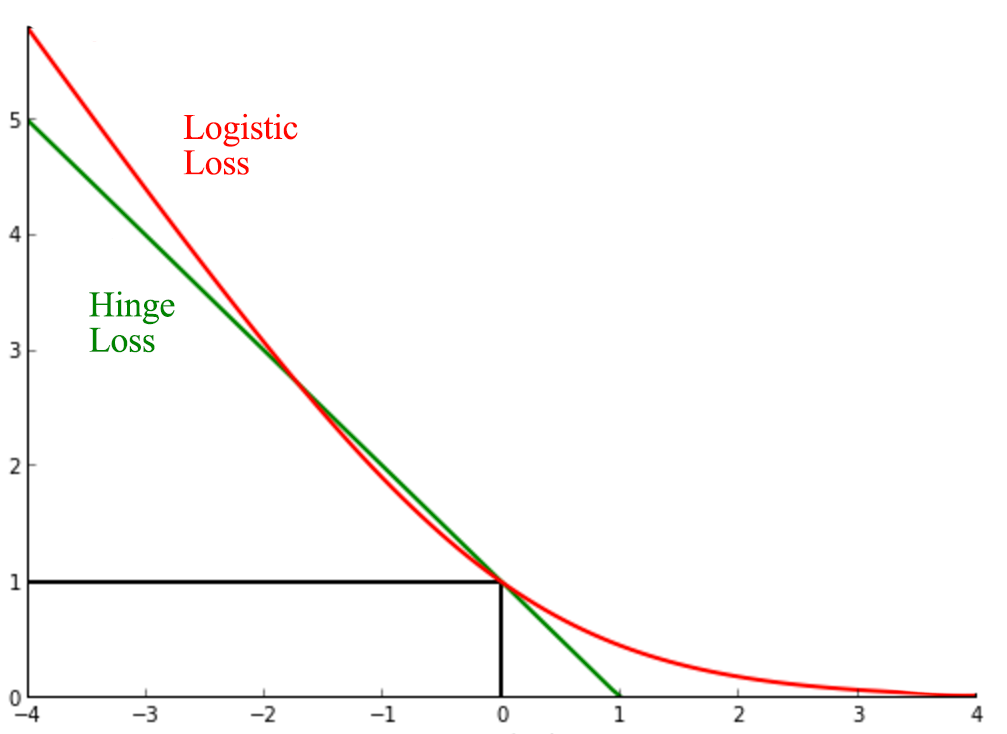
\includegraphics[width=0.4\textwidth]{images/losses-graph.png}
    \caption{Binary, Hinge, and logistic loss for $y'=1$}
\end{wrapfigure}
This loss function is however not convex in $\beta$; therefore, the problem of minimizing $\emrisk_n$ is extremely hard to solve. 
The idea of logistic regression consists in replacing the binary loss with another similar loss function, which is convex in $\beta$. This is the case of both the \emph{Hinge loss} and the \emph{logistic loss} which we will now introduce.

\begin{definition}[Hinge loss]
    The \emph{Hinge loss} $\ell_H:\R\times\{-1, 1\}\to\R_+$ is such that it values to $0$ when both arguments have the same sign and that $|y|\geq1$ (confident prediction), and increases linearly when their signs differ or when $|y|<1$ (prediction not confident enough):
    \begin{equation}
        \ell_H(y, y') := \max(0, 1-yy')
    \end{equation}
\end{definition}

\begin{definition}[Logistic loss]
    The \emph{logistic loss} $\ell_l:\R\times\{0, 1\}\to\R_+$ is defined by:
    \begin{equation}
        \ell_l(y, y') := y'\log(1-e^{-y}) + (1-y')\log(1+e^y)
    \end{equation}
\end{definition}

The advantage of the logistic loss with respect to the Hinge loss is that it has a probabilistic interpretation, by modeling $\P(Y=1|X)$, where $(X, Y)$ is a couple of random variables following the law $(X_i, Y_i)$. We will see more on this in the lecture on Maximum Likelihood.

\begin{definition}[Logistic regression estimator]
    The logistic regression estimator is the solution of the following minimization problem:
    \begin{equation}
        \hat{\beta}_{\textnormal{(logi.)}} := \argmin_{\beta\in\R^d}\frac{1}{n}\sum_{i=1}^n \ell_l(X^\tp_i\beta, Y_i)
    \end{equation}    
\end{definition}

\subsubsection{Computation of the estimator}
Similarly to OLS, we may try to analyticall solve the minimization problem to find $\hat{\beta}_{(\textnormal{logi.})}$. This could be done by cancelling the gradient of the empirical risk. Note that:
\begin{equation*}
    \frac{\partial\ell_l(y, y')}{\partial y} = \sigma(y)-y'
\end{equation*}
where $\sigma$ is the logistic function
\begin{equation*}
    \sigma = z \longmapsto \frac{1}{1+e^{-z}}.
\end{equation*}
Therefore,
\begin{equation*}
    \nabla\emrisk_n(\beta) = \frac{1}{n}\sum_{i=1}^nX_i(\sigma(X_i^\tp\beta)-Y_i)=\frac{1}{n}X(Y-\sigma(X\beta))
\end{equation*}
where $\sigma(X\beta)_i:=\sigma(X_i^\tp\beta)$. The problem is that the equation $\nabla\emrisk_n(\beta)=0$ had no closed-form solution. Therefore, it needs to be solved through iterative algorithms (gradient descent, Newton's method, \dots). Fortunately, this is possible, since the logistic loss is convex in its first argument. Indeed:
\begin{equation*}
    \frac{\partial^2\ell_l(y, y')}{\partial y^2} = \sigma(y)\sigma(-y)>0
\end{equation*}
Furthermore, the loss being strictly convex, the solution is even unique. In this chapter and in the next one, we will see tools and methods to solve convex optimization problems.

\subsubsection{Regularization}
Similarly to linear regression, logistic regression may over-fit the data (especially when $p>n$). In this case, one needs to add a regularization term, such as $\lambda\norm{\beta}^2_2$ to the logistic loss.

\subsection{Convex analysis}
\subsubsection{Convexity and minimization problems}
We will now see notions of convex analysis to solve convex optimization problems, such as logistic regression. This chapter will introduce convex analysis -- the properties of convex functions and convex optimization problems, and the next chapter will approach convex optimization algorithms (gradient descent, Newton's method, stochastic gradient descent, \dots).
\begin{wrapfigure}[10]{l}{0.4\textwidth}
    \centering
    \captionsetup{justification=centering}
    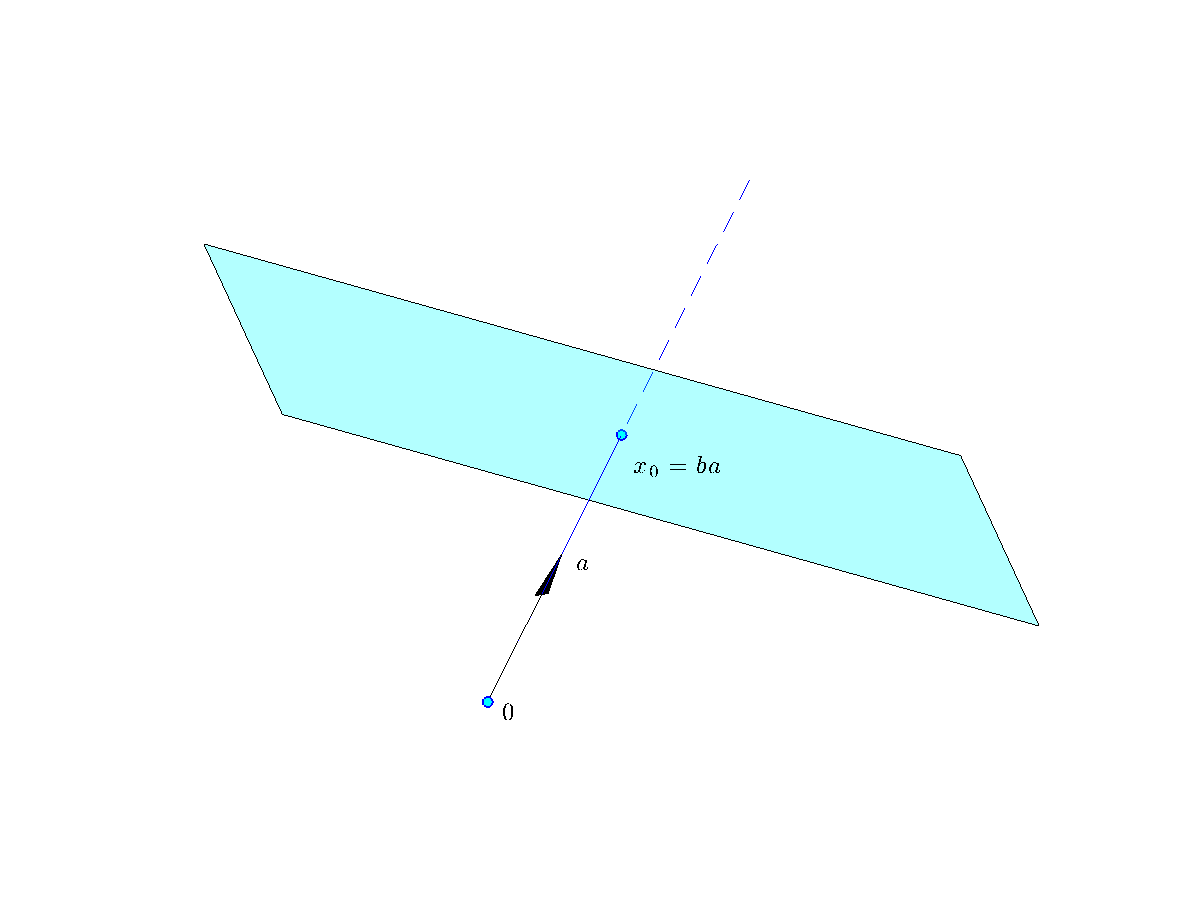
\includegraphics[width=0.3\textwidth]{images/hyperplane.png}
    \caption{Hyperplane}
\end{wrapfigure}

Convexity is a crucial notion in many fields of mathematics and computer science. In machine learning, convexity creates well-defined problems with efficient solutions. A typical example is the problem of \emph{empirical risk minimization}:
\begin{equation*}
    \hatf_n\in\argmin_{f\in\F}\frac{1}{n}\sum_{i=1}^n\ell(f(X_i), Y_i)+\lambda\Omega(f)
\end{equation*}
where $D_n=\set{(X_i, Y_i)}{i\in\iset{1}{n}}$ is the data set, $\F$ is a \emph{convex} set of predictors $f:\X\to\R$, for all $y'\in\Y$, $y\mapsto\ell(y, y')$ is a convex loss function, and $\Omega$ is a convex penaly (such as $\norm{\cdot}_2$, $\norm{\cdot}_1$, \dots).

Convexity will be useful to analyze bot statistical properties of the solution $\hatf_n$ and its generalization error:
\begin{equation*}
    \risk(\hatf_n):=\E[\ell(f(X), Y)|D_n]
\end{equation*}
but also to derive efficient algorithms to solve the forementionned minimization problem and find $\hatf_n$.

\subsubsection{Convex sets}
In what follows, we will only consider finite dimensional Euclidean spaces (typically $\R^d$).
\begin{wrapfigure}{r}{0.4\textwidth}
    \centering
        \captionsetup{justification=centering}
        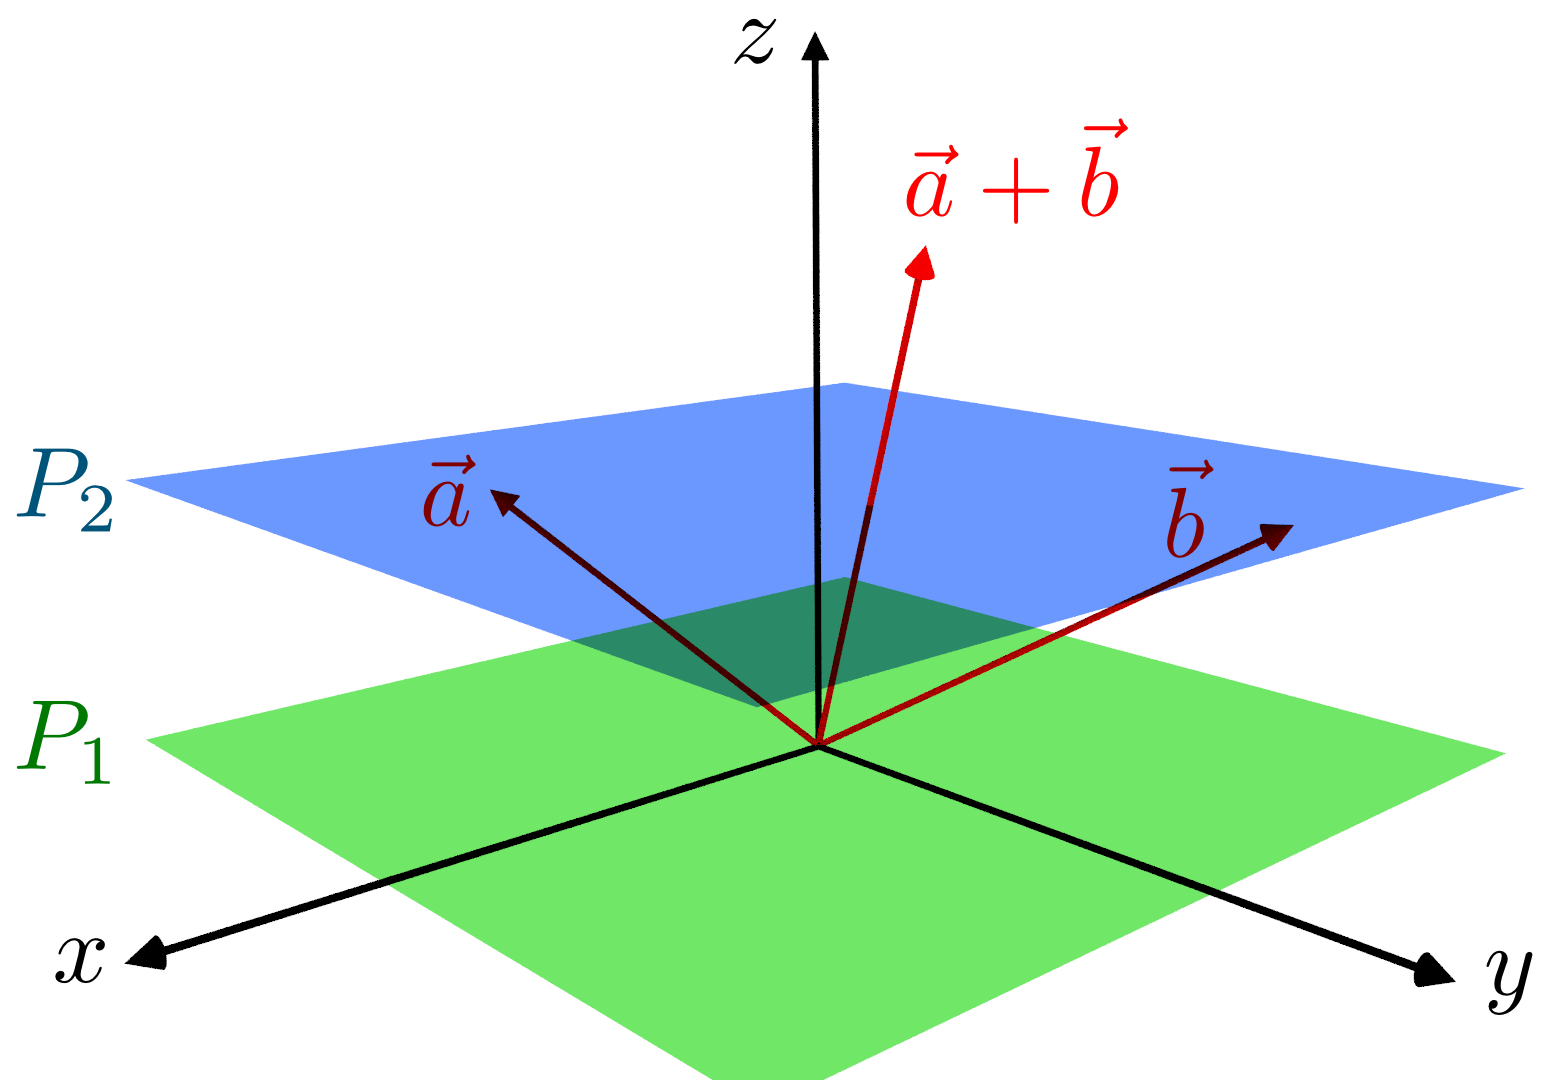
\includegraphics[width=0.35\textwidth]{images/affine-space.png}
        \caption{Affine space}
\end{wrapfigure}


\begin{definition}[Convex set]
    A set $K\subseteq\R^d$ is convex if and only if:
    \begin{equation*}
        \forall x, y\in K, \forall \alpha\in[0, 1], \quad \alpha x+(1-\alpha)y \in K
    \end{equation*}
    Said otherwise, $K$ is stable by barycentration, or, for all points $x, y\in K$, $[x, y]\subseteq K$.
\end{definition}

\begin{example}
    The following sets are convex:
    \begin{itemize}
        \item Hyperplans: $K=\set{x\in\R^d}{a^\tp x = b, a\neq 0, b\in\R}$
        \item Half spaces: $K=\set{x\in\R^d}{a^\tp x\geq b, a\neq0, b\in\R}$
        \item Affine subspaces: $K=\set{x\in\R^d}{Ax=b, A\in\mathscr{M}_d(\R), b\in\R}$
        \item Balls: $\set{x\in\R^d}{\norm{x}\leq R}$
        \item Cones: $K=\set{(x, r)\in\R^{d+1}}{\norm{x}\leq r}$
        \item Convex polytopes: intersections of half spaces
    \end{itemize}
\end{example}

\begin{wrapfigure}{l}{0.3\textwidth}
    \centering
        \captionsetup{justification=centering}
        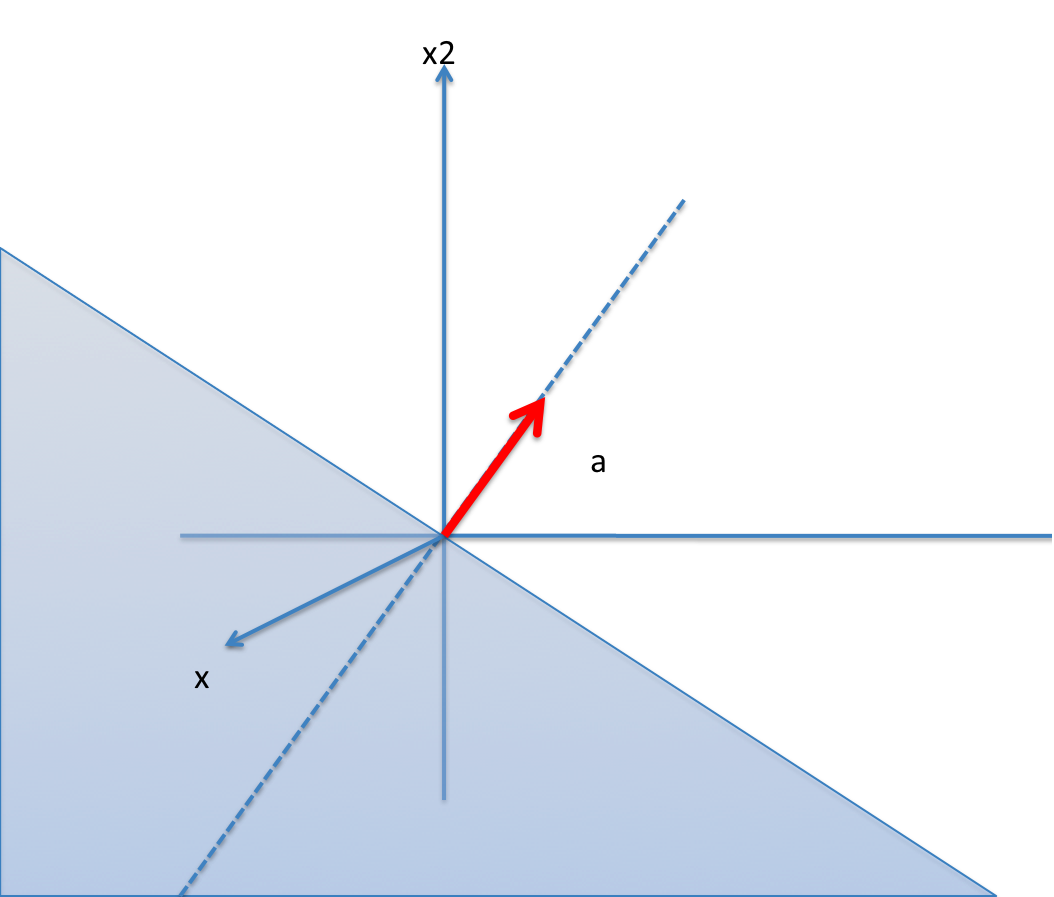
\includegraphics[width=0.3\textwidth]{images/half-space.png}
        \caption{Half-space}
\end{wrapfigure}
We know ennounce useful properties of convex sets.
\begin{property}[Stability by intersection]
    Convexity is stable by intersection. If $(K_i)_{i\in I}$ is a collection -- non-necessarily countable -- of convex sets, then:
    \begin{equation*}
        \bigcap_{i\in I}K_i \quad\textnormal{is convex}
    \end{equation*}
\end{property}

\begin{property}[Stability by affine transformation]
    Convexity is stable by affine transformation. If $K\subseteq\R^d$ is a convex set, then for all $\lambda\in\R$ and $\beta\in \R^d$,
    \begin{equation*}
        \lambda\cdot K+\beta := \set{\lambda\cdot x+\beta}{x\in K} \quad \textnormal{is convex}
    \end{equation*}
\end{property}

\begin{property}[Convex serparation]
    If $C$, $D$ are disjoints convex sets (i.e. $C\cap D=\emptyset$), then there exists a hyperplane which separates $C$ and $D$:
    \begin{equation*}
        \exists a\neq0, b\in\R, \quad C\subseteq\set{x\in\R^d}{a^\tp x\geq b}, D\subseteq\set{x\in\R^d}{a^\tp x\leq b}
    \end{equation*}
    Moreover, the inequalities are strict if $C$ and $D$ are compact.
\end{property}

\begin{wrapfigure}{r}{0.3\textwidth}
    \centering
        \captionsetup{justification=centering}
        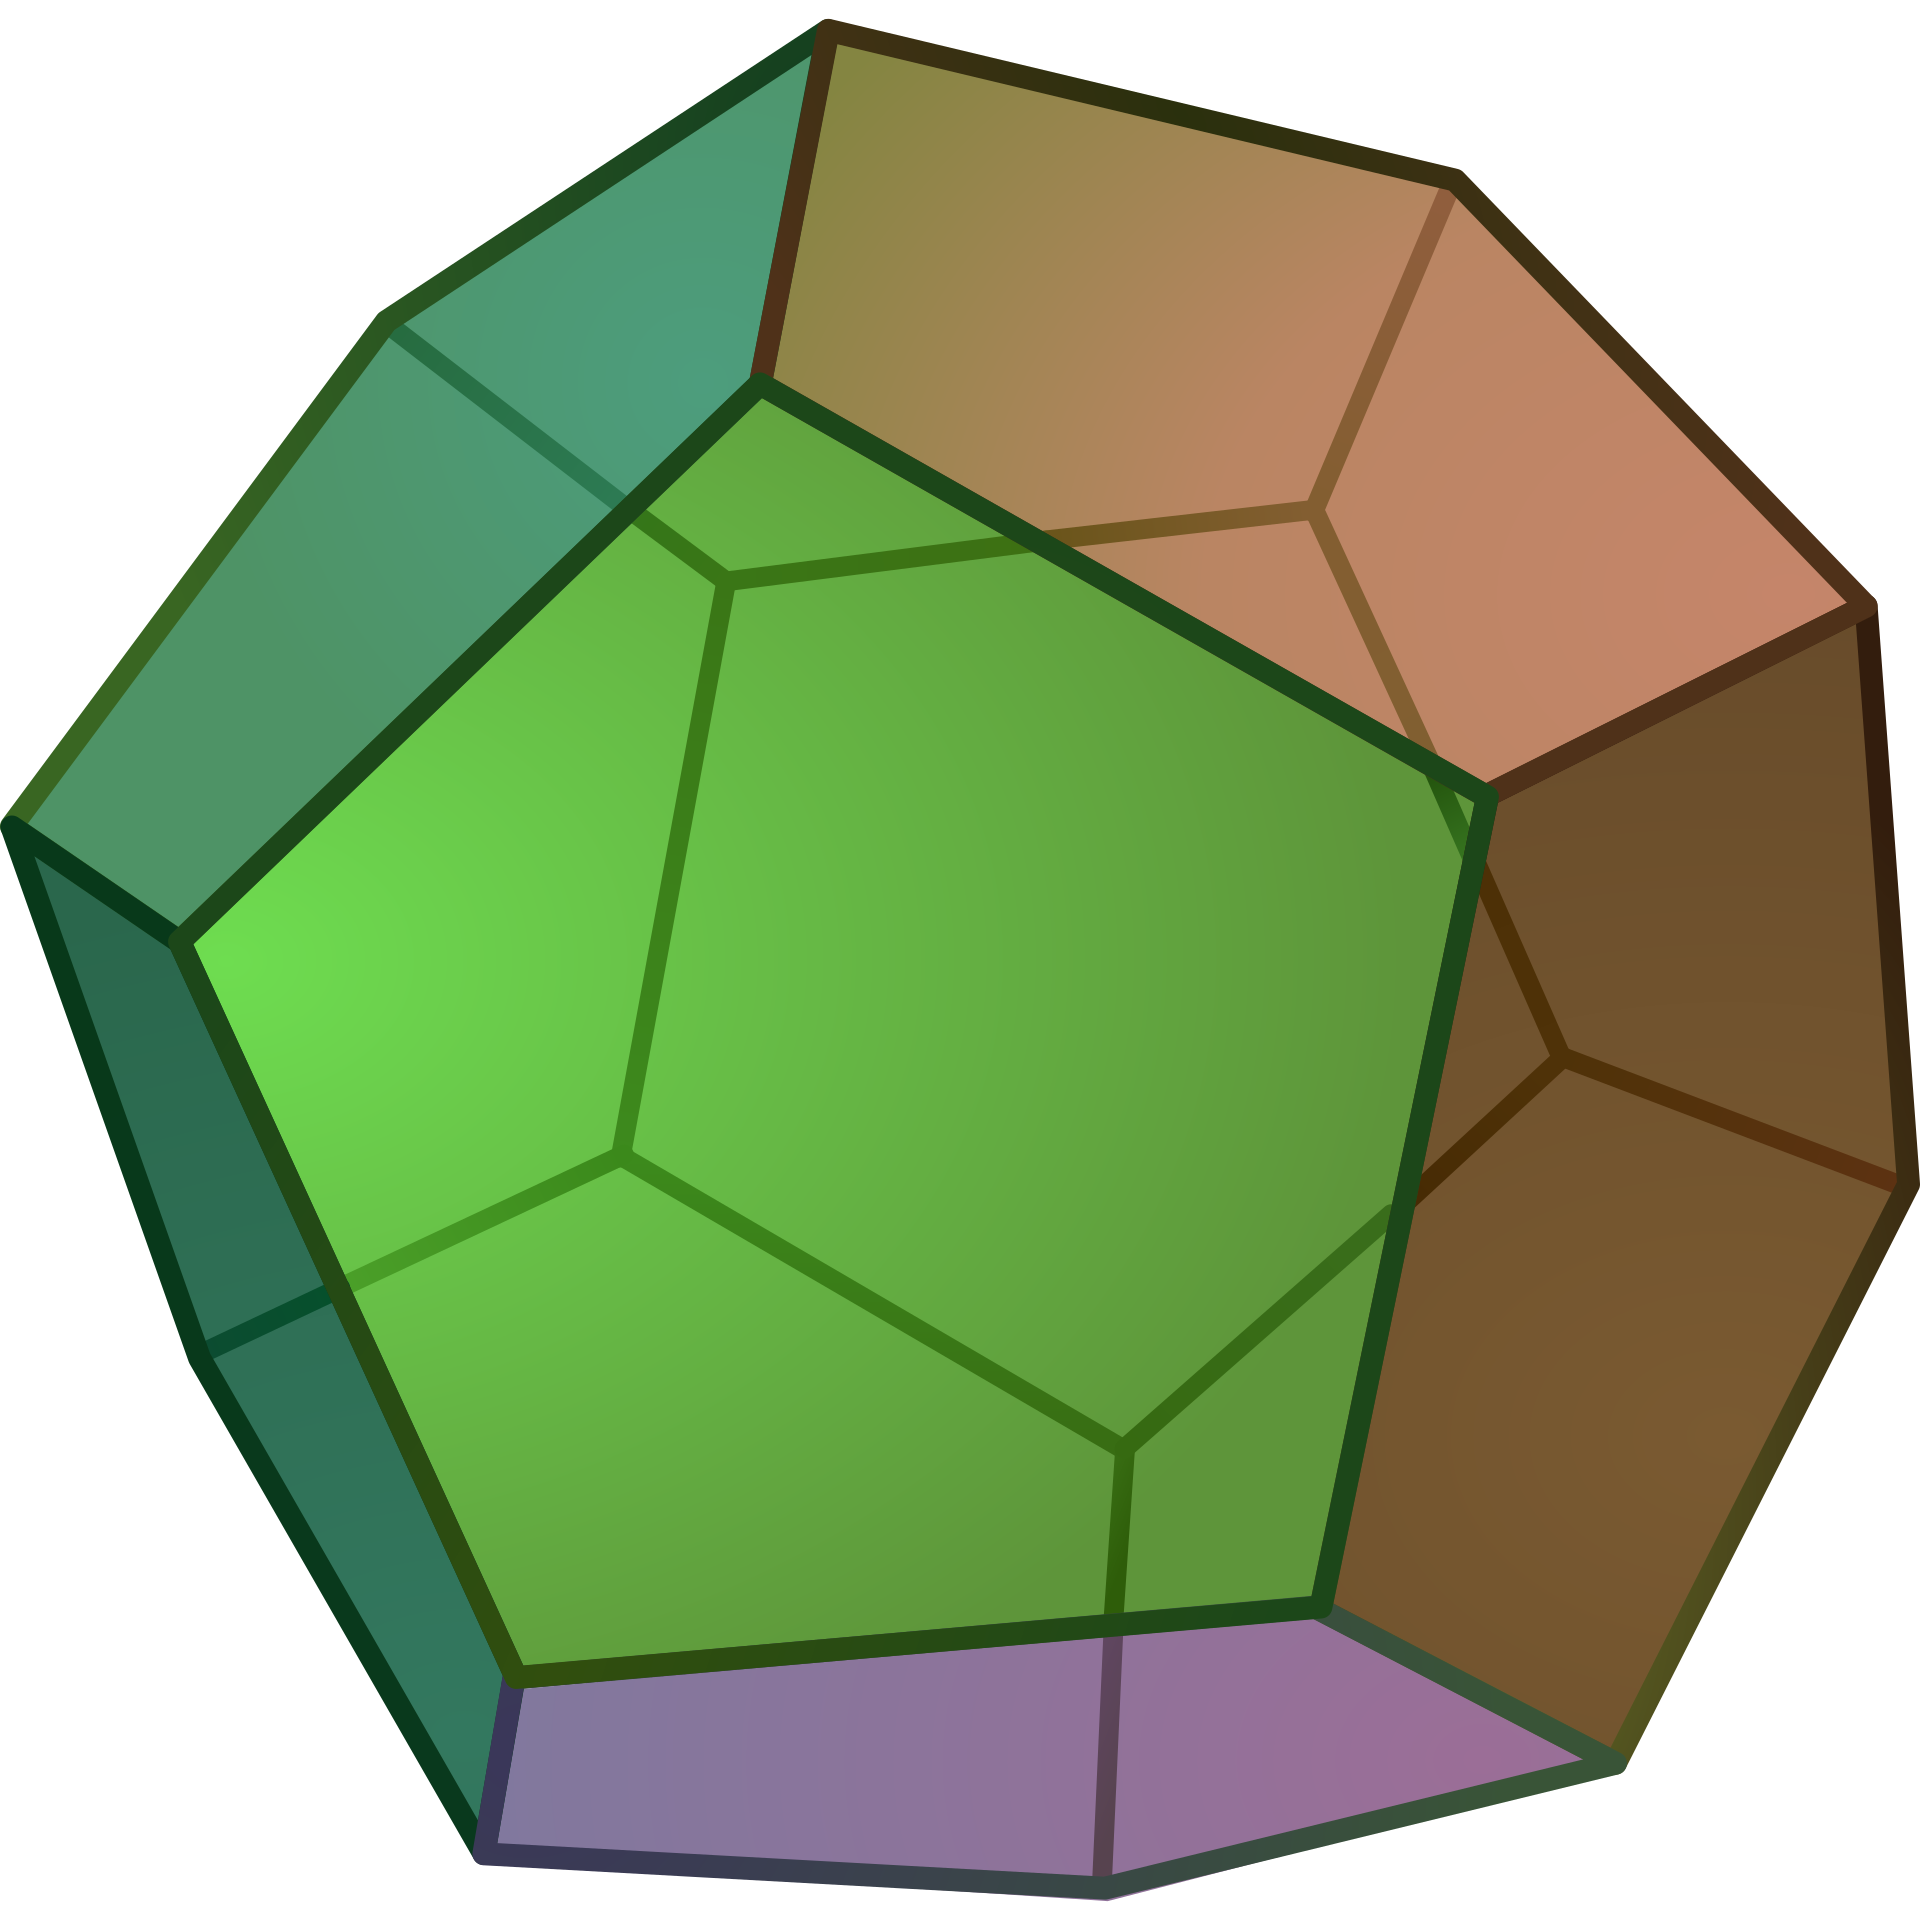
\includegraphics[width=0.2\textwidth]{images/polytope.png}
        \caption{Polytope}
\end{wrapfigure}
When a set is not convex, a trick is to use its convex hull to show some properties on it.
\begin{definition}[Convex Hull]
    Let $A\in\R^d$. The \emph{Convex Hull} of $A$, denoted $\Conv(A)$, is the smallest convex set that contains $A$. In other words,
    \begin{equation*}
        \begin{aligned}
            \Conv(A):=&\,\bigcap\set{B\in\R^d}{A\subseteq B, B \textnormal{ convex}}\\
            =&\,\set{\sum_{i=1}^p\alpha_iz_i}{p\geq 1, \alpha\in\R_+^p, (z_1, \dots, z_p)\in A^p, \; \sum_{i=1}^p \alpha_i=1}
        \end{aligned}
    \end{equation*}
\end{definition}

\subsubsection{Convex functions}
\begin{definition}[Convex function]
    A function $f:D\subseteq\R^d\to\R$ where $D$ is convex is a \emph{convex function} when:
    \begin{equation}
        \forall x, y \in D, \forall \alpha\in[0, 1], \quad f(\alpha x+(1-\alpha)y)\leq\alpha f(x) + (1-\alpha)f(y)
    \end{equation}
\end{definition}

\begin{definition}[Stricly convex function]
    A function $f:D\subseteq\R^d\to\R$ where $D$ is convex is a \emph{strictly convex function} when:
    \begin{equation}
        \forall x, y \in D, \forall \alpha\in[0, 1], \quad f(\alpha x+(1-\alpha)y)<\alpha f(x) + (1-\alpha)f(y)
    \end{equation}
\end{definition}

\vspace*{-0.5cm}
\begin{figure}[H]
    \centering
    \captionsetup{justification=centering}
    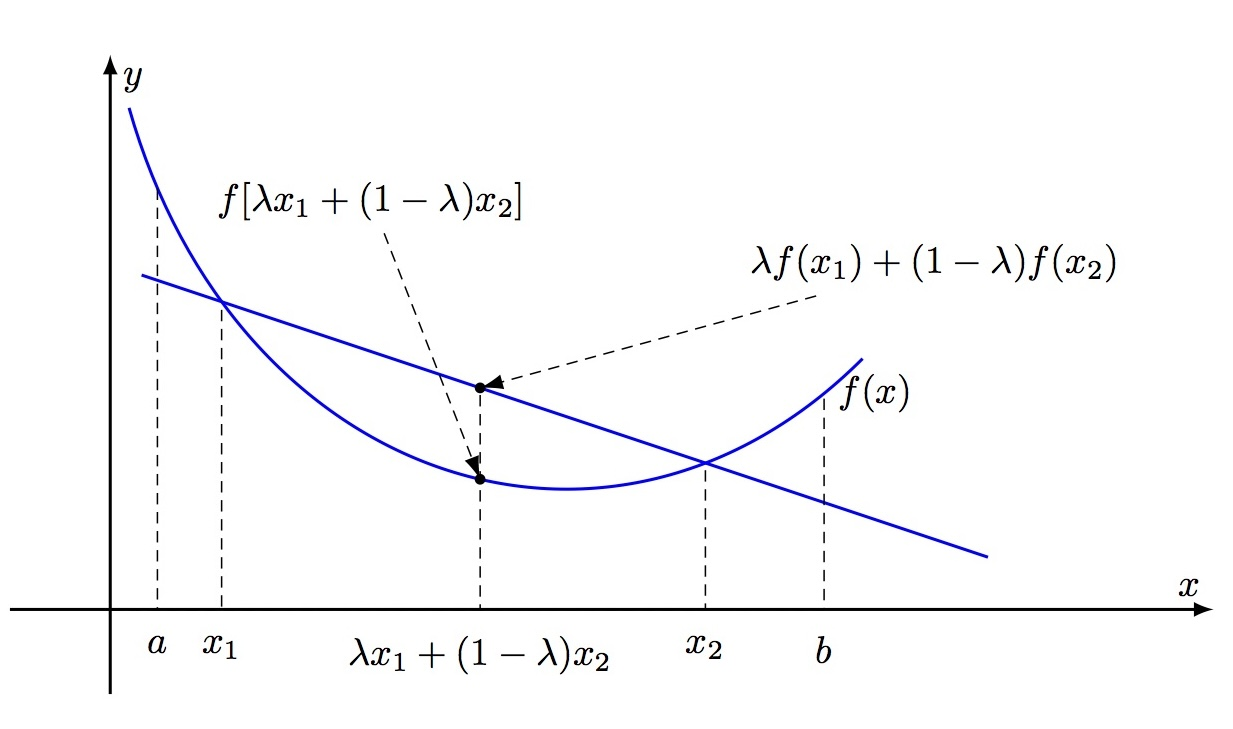
\includegraphics[width=0.7\textwidth]{images/convexity.jpg}
    \caption{Geometric interpretation of convexity}
\end{figure}

\begin{definition}
    A function $f:D\subseteq\R^d\to\R$ where $D$ is convex is \emph{$\mu$-stricly convex} when 
    \begin{equation*}
        x\longmapsto f(x)-\frac{\mu}{2}\norm{x}^2 \quad\textnormal{is convex}
    \end{equation*}
\end{definition}

\begin{example}[Convex functions]
    \leavevmode
    All the following functions are convex:
    \begin{figure}[H]
        \centering
        \begin{tabular}{c c}
            \begin{minipage}{0.45\textwidth}
                \vspace*{-0.4cm}
                In dimension $d=1$:
                \begin{itemize}
                    \item $x\longmapsto x$
                    \item $x\longmapsto x^2$
                    \item $x\longmapsto -\log(x)$
                    \item $x\longmapsto \log(1+e^{-x})$
                    \item $x\longmapsto |x|^p$ for $p\geq1$
                    \item $x\longmapsto -x^p$ for $p<1$
                \end{itemize}
            \end{minipage}
            \begin{minipage}{0.5\textwidth}
                Higher dimensions $d\geq1$:
                \begin{itemize}
                    \item Linear functions $x\longmapsto aa^\tp x$
                    \item Quadratic functions $x\longmapsto x^\tp Qx$ for $Q$ semidefinite symmetric positive matrix
                    \item Norms
                    \item $x\longmapsto\max\set{x_i}{i\in\iset{1}{d}}$
                    \item $x\longmapsto\log\left(\sum_{i=1}^de_i^x\right)$
                \end{itemize}
            \end{minipage}
        \end{tabular}
    \end{figure}
\end{example}

In practice, the functions which we will consider will be $\mathcal{C}^1$ and even $\mathcal{C}^2$. In this case, much simpler characterization are given for convex functions.

\begin{property}[Differentiable convex functions]
    If $f$ is $\mathcal{C}^1$,
    \begin{equation*}
        f \textnormal{ convex} \iff \forall x, y\in D, f(x)\geq f(y) + f'(y)(x-y)
    \end{equation*}
\end{property}
\begin{property}[Twice differentiable convex functions]
    If $f$ is twice differentiable,
    \begin{center}
        $f$ convex $\iff$ $\forall x\in D$, its Hessian is semi-definite positive ($f''(x)\geq0$)
    \end{center}
\end{property}

\begin{property}[Operations which preserve convexity]
    If $(f_i)_{i\in I}$ is a family of convex functions, then,
    \begin{equation*}
        x \longmapsto \sup_{i\in I} f_i(x) \quad\textnormal{is convex}
    \end{equation*}
    \begin{equation*}
        \forall \alpha_i\in\R_+, x \longmapsto \sum_{i\in I} \alpha_i f_i(x) \quad\textnormal{is convex}
    \end{equation*}
    Furthermore, if $f$ is convex on $C\times D$, then
    \begin{equation*}
        y \longmapsto \inf_{x\in C} f(x, y) \quad \textnormal{is convex on $D$}
    \end{equation*}
\end{property}

\begin{property}[Convexity and continuity]
    If $f$ is convex on $D$, then $f$ is continuous on $\mathring{D}$. Furthermore, the epigraph of $f$,
    \begin{equation*}
        \set{(x, t)\in D\times\R}{f(x)\leq t} \quad \textnormal{is convex.}
    \end{equation*}
\end{property}

\begin{property}[Jensen's inequality]
    For $f$ convex, $x_1, \dots, x_n\in D$ and $\alpha_1,\dots, \alpha_n\in\R_+$ such that $\sum_{i=1}^n\alpha_i=1$. Then:
    \begin{equation*}
        f\left(\sum_{i=1}^n\alpha_ix_i\right) \leq \sum_{i=1}^n\alpha_if(x_i)
    \end{equation*}
\end{property}

\begin{property}[Jensen's integral inequality]
    For $f$ convex, $p(x)\geq0$ over $S\subseteq D$ such that $\int_s p(x)\dd x=1$, then:
    \begin{equation*}
        f\left(\int_Sp(x)\,\dd x\right) \leq \int_Sp(x)f(x)\dd x
    \end{equation*}
\end{property}

\begin{property}[Jensen's expectation inequality]
    For $f$ convex, and $X$ a random variable such that $X\in D$ almost surely and with $\E[X]<+\infty$, then:
    \begin{equation*}
        f(\E[X])\leq\E[f(X)]
    \end{equation*}
\end{property}

\subsubsection{Unconstrained optimization problems}
Let $f:\R^d\to\R$ be a convex function. We consider the following minimization problem:
\begin{equation*}
    \inf_{x\in\R^d}f(x)
\end{equation*}
Note that the notation $\min_x f(x)$ is only used when the minimum is reached. If no point achieves the minimum, we use the notation $\inf_xf(x)$.

Three cases are possible, depending on $\inf_xf(x)$:
\begin{itemize}
    \item $\inf_{x\in\R^d}f(x)=-\infty$ -- there is no minimum.
    \item $\inf_{x\in\R^d}f(x)>-\infty$ and the minimum is not reached.
    \item $\inf_{x\in\R^d}f(x)>-\infty$ and the minimum is reached and equals $\min{x\in\R^d}f(x)$.
\end{itemize}

\begin{definition}[Local minimum]
    Let $f:D\to\R$ and $x\in D$. $x$ is a local minimum if and only if there exists an open set $V\subseteq D$ such that $x\in V$ and $f(x)=\min_{x'\in V}f(x')$.
\end{definition}

\begin{property}
    \label{prop:local-global-min}
    If $f$ is convex, any local minimum of $f$ is a global minimum.
\end{property}

\begin{property}
    If $f$ is stricly convex, it has at most one minimum.
\end{property}

\begin{property}
    If $f$ is convex and $\mathcal{C}^1$, then $x$ is a minimum of $f$ on $\R^d$ if and only if $f'(x)=0$.
\end{property}

\begin{figure}[H]
    \centering
    \captionsetup{justification=centering}
    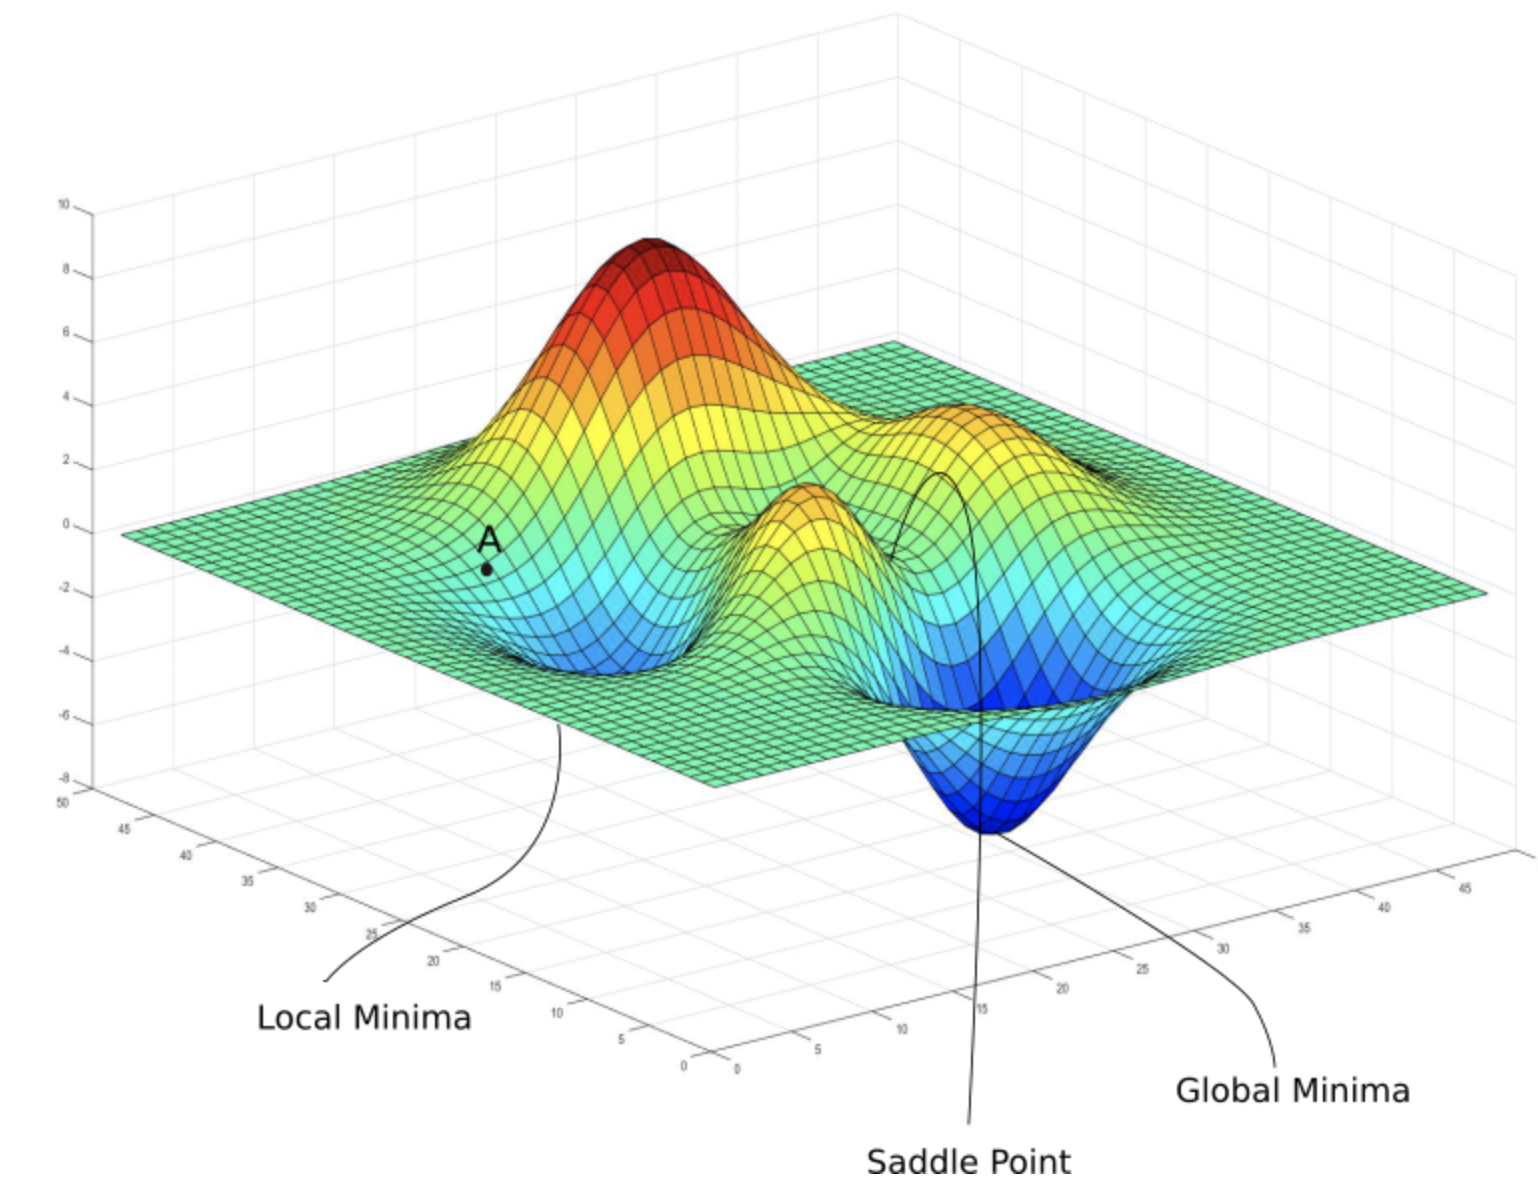
\includegraphics[width=0.7\textwidth]{images/local-minimum.png}
    \caption{Local and global minima of a non-convex function}
\end{figure}
These three properties justify the apprach of canceling the gradient to efficiently find a solution to a minimization problem. Property \ref{prop:local-global-min} guarantees that the result of some gradient descent is a global minimum, and not just some dead-end for the descent path. Strict convexity guarantees that every converging gradient descent will end up at the same minimum.

In the next chapter, we will continue the analysis of this frequent minimization problem and develop formal tools and algorithm to solve it efficiently.

\section{Convex analysis and convex optimization}
\subsection{Constrained optimization problems}
Let $f:D\mapsto\R^d$ convex and $C\subseteq D$ convex. We consider the constrained minimization problem
\begin{equation*}
    \inf_{x\in C}f(x)
\end{equation*}
where $C$ is the constraint set. It is often  defined as the intersection of sets of the form $\set{h_i(x)=0}{i\in I}$ (hyperplanes) and $\set{g_j(x)\leq0}{j\in J}$ (half-spaces).

\begin{example}[Minimization of a linear function over a compact]
    Let $A\subseteq\R^d$ be a compact, non-necessarily convex set, and $a\in\R^d\setminus\{0\}$. We can reformulate the non-convex minimization problem on $A$ as a constrained convex optimization problem on $\Conv(A)$:
    \begin{equation*}
        \min\set{a^\tp x}{x\in A} = \min\set{a^\tp x}{x\in\Conv(A)}
    \end{equation*}    
\end{example}

\subsubsection{Lagrangian duality}
A useful notion to solve constrained problems is Lagrangian duality. Assume that we are interested in the following constrained optimization problem:
\begin{equation}
    \label{eq:optimization-problem}
    \min_{x\in D}f(x) \quad \textnormal{such that}\quad 
    \begin{cases*}
        \tag{P}
        h_i(x) = 0 & for $i\in\iset{1}{m}$\\
        g_j(x)\leq0 & for $j\in\iset{1}{r}$
    \end{cases*}
\end{equation}
We denote by $D^*\subseteq D$ the set of points that satisfy the constraints:
\begin{equation*}
    D^* := \set{x\in D}{\forall i\in\iset{1}{m}, h_i(x)=0 \land \forall j\in\iset{1}{r}, g_j(x)\leq 0}
\end{equation*}
Note that the equality constraints $h_i(x)=0$ can be rewritten as inequalities:
\begin{equation*}
    h_i(x)\leq0 \land -h_i(x)\leq0
\end{equation*}
Unlike unconstrained optimization problems, canceling the gradient does not necessarily provide a solution for constrained optimization problems. The basic idea of Lagrangian duality is therefore to take the constraint $D^*$ into account in the minimization problem by augmenting the objective function with a weighted sum of the constraint functions.

\begin{figure}
    \centering
    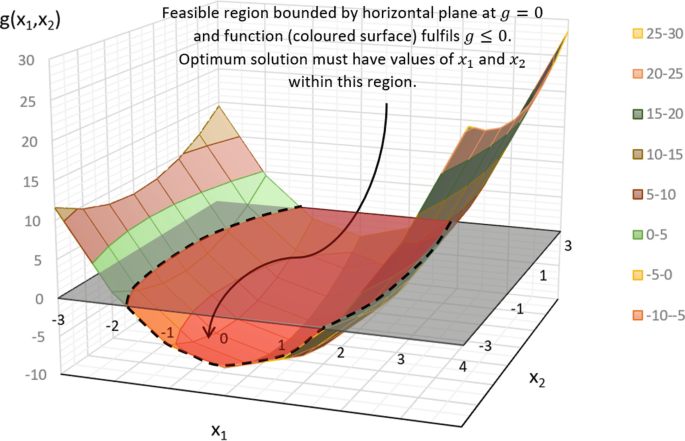
\includegraphics[width=0.7\textwidth]{images/constrained-optimization.png}
    \caption{Constrained optimization: $D^*$ is the red and orange part below the $g$ plane}
\end{figure}

\begin{definition}[Lagrangian]
    The \emph{Lagrangian} associated to the optimization problem \eqref{eq:optimization-problem} is the function
    \begin{equation*}
        \L:D\times\R^m\times\R_+^r \longrightarrow \R
    \end{equation*}
    defines by:
    \begin{equation*}
        \L(x, \lambda, \mu) = f(x) + \lambda^\tp h(x) + \mu^\tp g(x)
    \end{equation*}
\end{definition}

\begin{definition}[Primal function]
    We define the \emph{primal function} associated to \eqref{eq:optimization-problem}
    \begin{equation*}
        \bar{f}:D\longrightarrow\R\cup\{+\infty\}
    \end{equation*}
    by:
    \begin{equation*}
        \bar{f} : x \longmapsto \sup_{\lambda\in\R^m, \;\mu\in\R^r_+} \L(x, \lambda, \mu) = \begin{cases*}
            f(x) & if $x\in D^*$\\
            +\infty & otherwise
        \end{cases*}
    \end{equation*}
\end{definition}

\begin{definition}[Primal problem]
    With these definitions, we observe that the optimization problem \eqref{eq:optimization-problem} can be re-written as a constraints-free problem of minimization of the primal function.
    \begin{equation*}
        \begin{aligned}
            \inf_{x\in D^*} &= \inf_{x\in D}\bar{f}(x)\\
            &= \inf_{x\in D} \sup_{\lambda\in\R^m, \;\mu\in\R^r_+} \L(x, \lambda, \mu)
        \end{aligned}
    \end{equation*}
\end{definition}

\begin{definition}[Dual problem]
    The \emph{Dual problem} is obtained by exchanging inf and sup in the primal problem:
    \begin{equation*}
        \sup_{\lambda\in\R^m, \;\mu\in\R^r_+} f^*(\lambda, \mu) := \sup_{\lambda\in\R^m, \;\mu\in\R^r_+} \inf_{x\in D}\L(x, \lambda, \mu)
    \end{equation*}
    where
    \begin{equation*}
        f^* : (\lambda, \mu) \longmapsto \inf_{x\in D}\L(x, \lambda, \mu)
    \end{equation*}
    is the \emph{dual function}. If $f$ is convex, this function is concave. Note that the dual of the dual is the primal.
\end{definition}

The admissibility domain of the primal is $D^* := \set{x\in D}{\bar{f}(x)<+\infty}$, and the admissibility domain of the dual is $C^* := \set{(\lambda, \mu)\in\R^m\times\R_+^r}{f^*(\lambda, \mu)>-\infty}$. There is no solution to the optimization problem when $D^*=\emptyset$. The problem is unbounded when $C^*=\emptyset$.

\subsubsection{Link between primal and dual problems}
The primal and dual problems are not necessarily identical, but have a strong relationship. For any $(\lambda, \mu)$, $f^*(\lambda, \mu)$ provides a lower bound on the solution of \eqref{eq:optimization-problem}. The dual problem finds the best lower bound.

\begin{property}[Weak duality principle]
    \begin{equation*}
        d^* := \sup_{\lambda\in\R^m, \;\mu\in\R^r_+} \inf_{x\in D}\L(x, \lambda, \mu) \leq \inf_{x\in D} \sup_{\lambda\in\R^m, \;\mu\in\R^r_+} \L(x, \lambda, \mu)
    \end{equation*}    
\end{property}
The solution of the dual problem is therefore always smaller than the solution of the primal. A good mnemonic is to remember this inequality as \say{the largest dwarf is always smaller than the smallest giant}.

\begin{definition}[Dual gap]
    The \emph{dual gap} of the optimization problem is the difference between the primal and dual solutions:
    \begin{equation*}
        p^*-d^* \geq 0
    \end{equation*}
\end{definition}

\begin{definition}[Strong duality]
    There is \emph{strong duality} when $p^*=d^*$. In this case, the two problems are equivalent -- they share the same solutions. The existence of the solultions are related with the existence of saddle point of the Lagrangian. Note that strong duality does not always hold.
\end{definition}

\subsubsection{Strong duality}
Sometimes, the dual problem is easier to solve than the primal problem. It is then useful to know if there is strong duality.

\begin{definition}[Strictly feasible point]
    A point $x_0\in D$ is \emph{strictly feasible} when:
    \begin{equation*}
        \exists x_0\in D, \quad \begin{cases*}
            h_i(x_0)=0 & $\forall i\in\iset{1}{m}$\\
            g_j(x_0)<0 & $\forall j\in\iset{1}{r}$
        \end{cases*}
    \end{equation*}
\end{definition}

\begin{theorem}[Slater's condition]
    If $f$ and $D$ are convex, $h_i$ are affine and $g_j$ are convex, then the existence of a strictly feasible point implies strong duality.
\end{theorem}

\begin{example}
    Let $D=\R^d_+$ and consider the following linear programming minimization problem:
    \begin{equation*}
        \min_{x\in D, \; Ax=b}c^\tp x
    \end{equation*}
    where $A\in\mathscr{M}_{m, d}(\R)$ and $b\in\R^m$. The constraints can be written as $Ax-b=0$. Therefore, the Lagrangian is:
    \begin{equation*}
        \L : (x, \lambda) \in \R_+^d \times \R^m \longrightarrow c^\tp x + \lambda^\tp(b-Ax)
    \end{equation*}
    The primal problem can be rewritten using the Lagrangian:
    \begin{equation*}
        \begin{aligned}
            \min_{x\in D, \; Ax=b}c^\tp x &= \min_{x\in D}\sup_{\lambda\in\R^m} c^\tp x+\lambda^\tp(b-Ax)\\
            &= \min_{x\in D}\sup_{\lambda\in\R^m} b^\tp\lambda+x^\tp(c-A^\tp\lambda)
        \end{aligned}
    \end{equation*}
    The problem is convex since the objective function is convex, and the equality constraints are affine. By Slater's condition, we can swap the $\min$ and the $\sup$, giving:
    \begin{equation*}
        \begin{aligned}
            \min_{x\in D, \; Ax=b}c^\tp x &= \sup_{\lambda\in\R^m} \min_{x\in D} c^\tp x+\lambda^\tp(b-Ax)\\
            &= \sup_{\lambda\in\R^m, \; A^\tp\lambda\leq c} b^\tp\lambda
        \end{aligned}
    \end{equation*}
    This is the dual formulation of the problem.
\end{example}

\subsubsection{Karush-Kuhn-Tucker optimality conditions}
We will now see conditions playing the same role as gradient cancelling for unconstrained optimization problems. These conditions will be useful to find equations to compute analytically the solutions of the minimization problem.

Assume that the function $f$, $h_i$, and $g_i$ are all differentiable. Let $x^*$, and $(\lambda^*, \mu^*)$ be any primal and dual solutions, and assume that there is strong duality.

\begin{property}[KKT1]
    Since $x^*$ minimizes $\L(x, \lambda^*, \mu^*)$ over $x$, its gradient must be canceled at $x^*$:
    \begin{equation}
        \tag{KKT1}
        \nabla f(x^*) + \sum_{i=1}^m \lambda_i^*\nabla h(x^*) + \sum_{j=1}^r\mu_j\nabla g_j(x^*)=0
    \end{equation}
\end{property}

\begin{property}[KKT2]
    Since $x^*\in D^*$ and $(\lambda^*, \mu^*)\in C^*$ are feasible we have:
    \begin{equation}
        \tag{KKT2}
        \begin{aligned}
            \forall i\in\iset{1}{m},& \quad h_i(x^*)=0\\
            \forall i\in\iset{1}{r},& \quad g_j(x^*)\leq0\\
            \forall j\in\iset{1}{r},& \quad \mu_j^*\geq0
        \end{aligned}
    \end{equation}
\end{property}

\begin{property}[KKT3]
    The \emph{complementary condition} holds, i.e.:
    \begin{equation}
        \tag{KKT3}
        \forall j\in\iset{1}{r}, \quad \mu^*_jg_j(x^*)=0
    \end{equation}
\end{property}
\begin{proof}
    By contradiction, if the complementary condition does not hold, we could improve $\mu^*$ by setting $\mu_j^*=0$, since $g_j(x^*)\leq0$ and $(\lambda^*, \mu^*)$ maximizes $\L(x^*, \lambda, \mu)$.
\end{proof}

These conditions are called the Karush-Kuhn-Tucker (KKT) conditions. When the primal problem is convex, these conditions are also sufficient.

\begin{theorem}[Karush–Kuhn–Tucker theorem]
    If there is strong duality, then:
    \begin{center}
        (KKT) conditions are satisfied $\iff$ $\begin{cases*}
            x^* &is a solution to the primal problem\\
            (\lambda^*, \mu^*) & is a solution of the dual problem
        \end{cases*}$
    \end{center}
\end{theorem}

The KKT conditions play an important role in optimization. In some cases, it is possible to solve them analytically. Many optimization methods are conceived for solving the KKT conditions.

\subsection{Optimization algorithms for unconstrained convex optimization}
In this section we will see two widely used optimization algorithms for the problem of unconstrained optimization, \emph{Gradient descent} and \emph{Stochastic Gradient descent}.

Since the goal of minimizing a function $f:\R^d\to\R$ for $d\in\N$ is to find the point $x$ for which the function has minimum value, the fundamental idea behind gradient descent consists in strating from a given $x_0\in\R^d$ and finding the next point following a descet direction iteratively. In particular, we will consider $f$ to be a convex function.

\subsubsection{Gradient Descent}
\begin{wrapfigure}[15]{l}{0.45\textwidth}
    \captionsetup{justification=centering}
    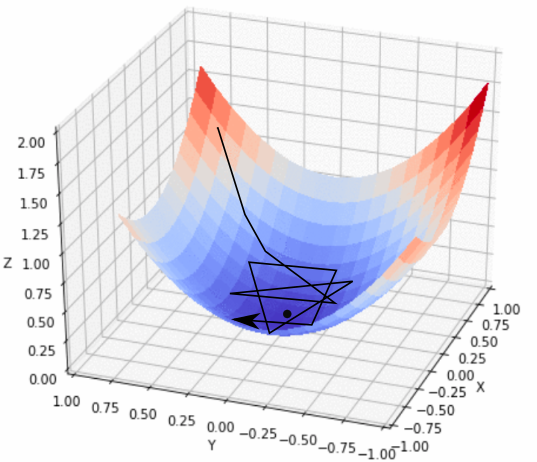
\includegraphics[width=0.4\textwidth]{images/gradient-descent-2.png}
    \caption{Convex gradient descent}
\end{wrapfigure}
When $f$ is diffenrentiable, the gradient of $f$ in $x$, denoted $\nabla f(x)$, determines the direction of maximum increase of the function in a suitable neighborhood of $x$ -- and so $-\nabla f(x)$ determines the direction of maximum decrease of the function. The gradient descent algorithm then reads as follows:
\begin{equation*}
    \begin{cases*}
        x_0 & given\\
        x_{t+1} := x_n -\gamma_t\nabla f(x_t) & $\forall t\in\iset{1}{T}$
    \end{cases*}
\end{equation*}
where $\gamma_n$ is denoted as \emph{step-size} and is small enough such that $-\gamma_t\nabla f(x_t)$ is still a decrease direction in the neighborhood of $x_t$.

The choice of $\gamma_t$ is crucial for the optimization algorithm. If $\gamma_t$ is too big, it makes the algorithm unstable and possibly divergince, since it follows the direction $-\nabla f(x_t)$ out of the region where it is a descent direction. On the other hand, if $\gamma_t$ is too small, the chosen direction is a descent direction, but each step is very short, leading to a larger number of steps required to arrive to the minimum solution -- with a big impact on the total computational complexity.

\begin{figure}[H]
    \centering
    \begin{minipage}{0.45\textwidth}
        \begin{tikzpicture}[scale=0.8]
            \draw[->, thick] (0,0) -- (7,0) node[below] {$x$};
            \draw[->, thick] (0,0) -- (0,6) node[left] {$f(x)$};

            \draw[domain=1.25:5.75, samples=50, thick] plot (\x, \x*\x-7*\x+13);

            \draw[dotted, thick] (3.5, 0.75) -- (3.5, 0) node[below] {$x^*$};
            \node at (3.5, 0.75)[circle,fill,inner sep=1.5pt]{};

            \foreach \n in {1.6,1.7,1.8,1.9,2,2.1,2.2,2.3,2.4,2.5,2.6,2.7}
                {
                    \draw[-, thick, color=red] (\n, \n*\n-7*\n+13)  -- (\n+0.1,\n*\n+\n*0.2-7*\n-0.7+13);
                    \node at (\n, \n*\n-7*\n+13)[circle,fill,inner sep=1.2pt, color=red]{};
                }
        \end{tikzpicture}
        \caption*{Too small: converges very slowly}
    \end{minipage}
    \begin{minipage}{0.45\textwidth}
        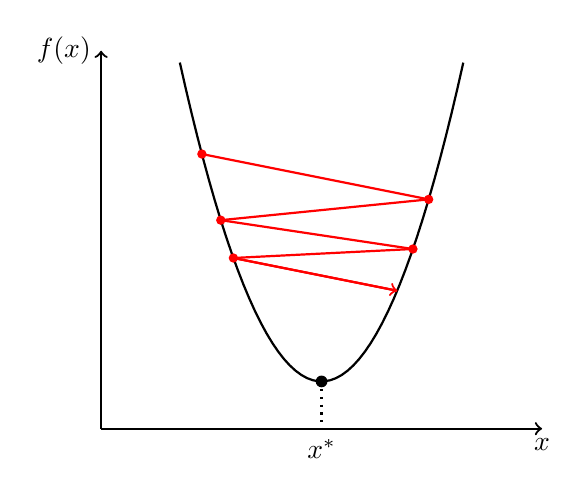
\begin{tikzpicture}[scale=0.8]
            \draw[->, thick] (0,0) -- (7,0) node[below] {$x$};
            \draw[->, thick] (0,0) -- (0,6) node[left] {$f(x)$};

            \draw[domain=1.25:5.75, samples=50, thick] plot (\x, \x*\x-7*\x+13);

            \draw[dotted, thick] (3.5, 0.75) -- (3.5, 0) node[below] {$x^*$};
            \node at (3.5, 0.75)[circle,fill,inner sep=1.5pt]{};

            \foreach \i\j in {1.6/5.2,5.2/1.9,1.9/4.95,4.95/2.1,2.1/4.7}
            {
                \draw[-, thick, color=red] (\i, \i*\i-7*\i+13)  -- (\j, \j*\j-7*\j+13);
                \node at (\i, \i*\i-7*\i+13)[circle,fill,inner sep=1.2pt, color=red]{};
            }
            \draw[->, thick, color=red] (2.1, 2.1*2.1-7*2.1+13)  -- (4.7, 4.7*4.7-7*4.7+13);
        \end{tikzpicture}
        \caption*{Too big: overshoots and diverges}
    \end{minipage}
    \caption{Choice of step size}
\end{figure}

We will prove in the next theorem that there exists a step-size that guarantees the convergence of the solution of the gradient descent algorithm to the minimizer of $f$, and we characterize how fast gradient descent achieves it.

\subsubsection{Gradient Descent for strongly convex functions}
\begin{definition}[$L$-Lipschitz continuous gradients]
    For $L>0$, $f$ has $L$-Lipschitz continuous gradients when:
    \begin{equation*}
        \forall x, y, \in\R^d, \quad \norm{\nabla f(x) - \nabla f(y)}\leq L\norm{y-x}
    \end{equation*}
\end{definition}

\begin{lemma}
    Let $L>0$ and $f:\R^d\to\R$ be a convex function with $L$-Lipschitz continuous gradients, then:
    \begin{equation}
        f(y)\leq f(x)+\nabla f(x)^\tp(y-x)+L\norm{y-x}^2
    \end{equation}
\end{lemma}
\begin{proof}
    %TODO
\end{proof}

\begin{remark}
    Using a different argument, it is possible to prove the tighter result:
    \begin{equation}
        \label{eq:tighter-ineq}
        f(y)\leq f(x)+\nabla f(x)^\tp(y-x)+\frac{L}{2}\norm{y-x}^2
    \end{equation}
\end{remark}

\begin{lemma}[Gradient descent is a descent algorithm with $\gamma_t\in\openseg{0, 1/L}$]
    Let $f$ be convex with $L$-Lipschitz gradient, let $x_0\in\R^d$ and $\gamma_t>0$, then:
    \begin{equation*}
        \forall t\in\N^*, \quad f(x_t)\leq f(x_{t-1}) - \gamma_t(1-L\cdot\gamma_t) \cdot \norm{\nabla f(x_{t-1})}^2
    \end{equation*}
    In particular, if $\gamma_t\in\openseg{0, 1/L}$, we have that $\gamma_t(1-L\cdot\gamma_n)>0$. Therefore, for all $t\in\N^*$:
    \begin{equation*}
        f(x_t)<f(x_{t-1})
    \end{equation*}
    whenever $x_{t-1}$ is not a global optimum, otherwise $x_t=x_{t-1}$ and $f(x_t)=f(x_{t-1})$ (a fixpoint is reached).
\end{lemma}
\begin{proof}
    %TODO
\end{proof}

Recall that when $f$ is $\mu$-stricly convex, we have:
\begin{equation*}
    f(y)\geq f(x)+\nabla f(x)^\tp(y-x)+\frac{\mu}{2}\norm{y-x}^2
\end{equation*}
This will be used in the next theorem.

\begin{theorem}
    Let $f:\R^d\to\R$ be a $\mu$-stricly convex function with $L$-Lipschitz continuous gradients. Let $\gamma\in\openseg{0, 1/2L}$, and choose a constant step-size $\gamma_t:=\gamma$ for $t\in\N$. Denote by $x^*$ the global optimum of $f$. Finally, let $x_0\in\R^d$ and $T\in\N$. Then:
    \begin{equation*}
        \norm{x_T-x^*}^2\leq(1-\gamma\mu)^T\norm{x_0-x^*}^2
    \end{equation*}
\end{theorem}
\begin{proof}
    %TODO
\end{proof}

\begin{remark}
    Using the tighter inequality \eqref{eq:tighter-ineq}, the previous result can be extended to $\gamma\in\rbrack 0, 1/L\lbrack$.
\end{remark}

Note that since:
\begin{equation*}
    (1-\gamma\mu)^T\leq e^{-\gamma\mu T}
\end{equation*}
the choice of $T=\frac{\gamma\mu}\log(\norm{x_0-x^*}^2/\epsilon)$ gives:
\begin{equation*}
    \norm{x_T-x^*}^2\leq\epsilon
\end{equation*}

\begin{corollary}
    Under the same hypothesis on $f$, $\gamma$, we have:
    \begin{equation}
        \norm{x_T-x^*} \xrightarrow[T\to+\infty]{} 0
    \end{equation}
    Therefore, in this case, the Gradient Descent algorithm converges.
\end{corollary}

\subsubsection{Stochastic Gradient Descent}
In this section, we will introduce Stochastic Gradient Descent. In some cases, especially when $n$ is big, computing the actual gradient of the empirical risk function $\emrisk_n$ is extremely costly. The approach of SGD is therefore to replace the exact gradient by a stochastic approximation of it, in practice calculating it from a random subset of the training data. This enables faster iterations, at the cost of a slower convergence rate.

The algorithm is useful to find the global minimum of conex functions of the form
\begin{equation*}
    f(x)=\E_\theta\left[g(x, \theta)\right], \where \E_\theta\left[g(x, \theta)\right]=\int_\Omega g(x,\theta)\dd p(\theta)
\end{equation*}
where $p$ is a probability distribution over $\Omega$ and $g:\R^d\times\Omega\to\R$.

\begin{example}[Empirical Risk Minimization]
    We consider $f$ of the form:
    \begin{equation*}
        f(x) = \frac{1}{n}\sum_{i=1}^n L(x, \theta_i), \where \begin{cases}
            \theta_i=(z_i, y_i)\\
            L(x, \theta_i)=\ell(x^\tp z_i, y_i)
        \end{cases}
    \end{equation*}
\end{example}
In this context, we can assume that due to the size of $\Omega$ (in the previous example, $n$), we are not able to evaluate the integral above, but we assume that we are able to sample some $\theta_t$ from $p$ and to compute the gradient $\nabla_x g(x, \theta_t)$.

The algorithm is similar to classical gradient descent, but the iteration step is changed to:
\begin{equation*}
    x_t=x_{t-1}-\gamma_t\nabla_x g(x, \theta_t) \where \theta_t\sim p
\end{equation*}
As previously, $\gamma_t$ is a sequence of step sizes and $x_0$ is given; moreover, specifically for stochastic GD, $\theta_t$ is independently and identically distributed according to $p$. 

Note that, by linearity of the integral $\nabla f(x)=\E_\theta\left[\nabla_x g(x,\theta)\right]$, thus:
\begin{equation*}
    \begin{aligned}
        \E_\theta[x_t] &= x_{t-1}-\gamma_t\nabla_xg(x_{t-1},\theta_t)\\
        &=x_{t-1} - \gamma_t\nabla f(x_{t-1})
    \end{aligned}
\end{equation*}
Intuitively, the SGD seems to behave in expectation like gradient descent. Let's analyze this property in more details with the following theorem.

\begin{definition}[Variance of the estimator of the gradient]
    We define the \emph{variance of the estimator of the gradient} as:
    \begin{equation*}
        \sigma^2(x):=\E_\theta\left[\norm{\nabla f(x)-\nabla_x g(x,\theta)}^2\right]
    \end{equation*}
\end{definition}

\begin{theorem}[Expectation bound for SGD]
    Assuming that $f:\R^d\to\R$ is $\mu$-stricly convex and with $L$-Lipschitz continuous gradients, let $\gamma_t=\gamma$ for $t\in\N$, with $\gamma\in\openseg{0, 1/2L}$. Assume that there exists $\sigma^2_*$ such that
    \begin{equation*}
        \forall x\in\R^d, \quad \sigma^2(x)\leq\sigma^2_*
    \end{equation*}
    Under such assumptions, we have that:
    \begin{equation*}
        \E_{\theta_1,\dots,\theta_T}\left[\norm{x_T-x^*}^2\right] \leq (1-\mu\gamma)^T\norm{x_0-x^*}^2+\frac{\gamma}{\mu}\sigma^2
    \end{equation*}
\end{theorem}
\begin{proof}
    %TODO
\end{proof}

\begin{corollary}[Convergence of SGD]
    Under the same assumptions:
    \begin{equation*}
        \E_{\theta_1,\dots,\theta_T}\left[\norm{x_T-x^*}^2\right] \xrightarrow[T\to+\infty]{} 0
    \end{equation*}
    Hence, stochastic gradient descent converges in expectation towards the global minimum.
\end{corollary}

\section{Kernels}
\subsection{Introduction to kernels}
In this course, we often focused on prediction methods which are \emph{linear}, that is, the input data are vectors and the prediction function is linear (e.g. $f(x)=w^\tp x$ for $w\in\R^d$). In this situation with given data $(x_i, y_i)$, the vector $w$ can be obtained by minimizing
\begin{equation*}
    \hat{L}(w)=\frac{1}{n}\sum_{i=1}^n l(y_i, w^\tp x_i) + \lambda \Omega(w)
\end{equation*}

Classical examples are logistic regression or least-squares regression. These methods look at first sight of limited practical significance, because input data may not be vectors, and relevant prediction functions may not be linear.

The goal of kernel methods is therefore to go beyond these limitations while keeping the good aspects. The underlying principle is to replace $x$ by a function $\phi(x)\in\R^d$, \emph{explicitly} or \emph{implicitly}, and consider linear predictions in $\Phi(x)$, i.e.~$f(x)=w^\tp \phi(x)$. We call $\phi(x)$ the \emph{feature} associated to $x$.

\begin{example}[Linear regression]
    In the case of linear regression, $\phi(x)=x$ for $x\in\R^d$. As expected, this gives us linear models:
    \begin{equation*}
        f(x)=w^\tp x = \sum_{j=1}^d w_jx_j
    \end{equation*}
\end{example}

\begin{example}[Polynomial regression of degree $r$]
    With $x\in\R$, we have $\phi(x)\in\R^{r+1}$ defined by:
    \begin{equation*}
        \phi(x)=(1, x, x^2, \dots, x^r)
    \end{equation*}
    Therefore, the prediction functions will be general polynomials of degree at most $r$:
    \begin{equation*}
        f(x)=w^\tp\phi(x)=\sum_{j=0}^r (\phi(x))_j = \sum_{j=1}^r w_jx^j
    \end{equation*}
\end{example}

\begin{example}[Polynomial multivariate regression of degree $r$]
    We consider $x\in\R^d$ and
    \begin{equation*}
        \phi(x)=(x_1^{\alpha_1}, \dots, x_d^{\alpha_d}) \where \sum_{i=1}^d \alpha_i=r
    \end{equation*}
    In this situation, $p=\binom{d+r-1}{r}$ might be too big for an explicit representation to be feasible.
\end{example}

\begin{example}[Generic set of functions]
    Let $\varphi_1, \varphi_r : \R^d \to \R$ be a set of functions of interest (e.g. a subset of the Fourier basis); we define $\phi(x) = (\varphi_1(x), \dots, \varphi_r(x))$ to have:
    \begin{equation*}
        f(x)=w^\tp \phi(x) = \sum_{j=1}^rw_j\varphi_j(x)
    \end{equation*}
\end{example}

\subsection{Representer theorem}
\subsubsection{Theorem statement}
Given a dataset $x_1, \dots, x_n$, let $\phi$ be a feature map, such that we are able to compute the observed feature maps $\phi(x_1), \dots, \phi(x_n)$. We can ask ourselves if there exists an easier representation for $w$ in terms of these observed feature maps, i.e.~we want to know if it is possible to characterize the minimum $\hat{w}$ of:
\begin{equation*}
    \hat{L}(w) = \frac{1}{n}\sum_{i=1}^n l(y_i, w^\tp\phi(x_i)) + \lambda w^\tp w
\end{equation*}
in the form of $\hat{w} = \sum_{i=1}^n \alpha_i\phi(x_i)$, with $\alpha_i\in\R$. The following theorem guarantees such characterization under basic properties of $\hat{L}$.

\begin{theorem}[Representer theorem]
    Let $\phi:\X\to\R^d$. Let $(x_1, \dots, x_n)\in\X^n$ and assume that $\Psi:\R^{n+1}\to\R$ is strictly increasing with respect to the last variable. Then, the minimum of
    \begin{equation*}
        \hat{L}(w) := \Psi(w^\tp\phi(x_1), \dots, w^\tp\phi(x_n), w^\tp w)
    \end{equation*}
    is obtained for
    \begin{equation*}
        w=\sum_{i=1}^n \alpha_i \phi(x_i)
    \end{equation*} for some $\alpha\in\R^n$.
\end{theorem}

\begin{proof}
    % TODO
\end{proof}

\begin{corollary}
    For $\lambda>0$, 
    \begin{equation*}
        \min_{w\in\R^d} \frac{1}{n} \sum_{i=1}^n \ell(y_i, w^\tp\phi(x_i)) + \frac{\lambda}{2} w^\tp w
    \end{equation*}
    is obtained for
    \begin{equation*}
        w = \sum_{i=1}^n \alpha_i\phi(x_i).
    \end{equation*}
\end{corollary}

Note that there is no assumption on $\ell$, and in particular, no convexity assumption. This result is extendable to Hilbert spaces (RKHS\footnote{\emph{Reproducing kernel Hilbert space}, a specific kind of Hilbert space which is often used in machine learning.}), as we will see in the next section.

\subsubsection{Finite dimensional representation of the learning problem}
Using the representer theorem, we know that the minimum of $\hat{L}$ is of the form $w=\sum_{i=1}^n \alpha_i\phi(x_i)$; we can therefore directly optimize this characterization, i.e.~we can then write:
\begin{equation*}
    \min_{w\in\R^r} \frac{1}{n} \sum_{i=1}^n \ell(y_i, w^\tp\phi(x_i)) + \frac{\lambda}{2} w^\tp w = \min_{\alpha\in\R^n} \frac{1}{n}\sum_{i=1}^n \ell(y_i, (K\alpha)_i) + \frac{\lambda}{2}\alpha^\tp K\alpha
\end{equation*}
where $K\in\mathscr{M}_n(\R)$ with values
\begin{equation*}
    K_{i, j} = \phi(x_i)^\tp \phi(x_j).
\end{equation*}

Indeed,
\begin{equation*}
    \phi(x_i)^\tp w = \sum_{j=1}^n \alpha_j\phi(x_i)^\tp\phi(x_j) = (K\alpha)_i
\end{equation*}
moreover,
\begin{equation*}
    ||w||^2 = w^\tp w = \sum_{i=1}^n\sum_{j=1}^n \alpha_i\alpha_j\phi(x_i)^\tp\phi(x_j) = \alpha^\tp K\alpha
\end{equation*}

We finally have a closed form representation for the function evaluation. Defining the \emph{kernel function} $k(x, x'):=\phi(x)^\tp \phi(x')$, we have:
\begin{equation*}
    f(x) = w^\tp\phi(x) = \sum_{i=1}^n \alpha_i\phi(x_i)^\tp\phi(x) = \sum_{i=1}^n \alpha_i k(x_i, x).
\end{equation*}

\begin{figure}[H]
    \centering
    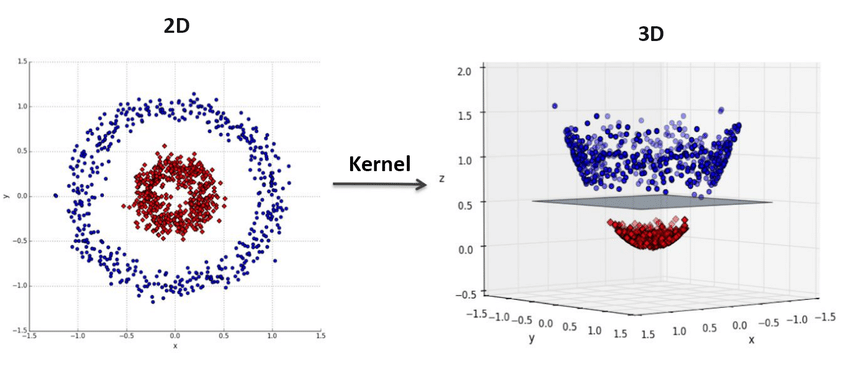
\includegraphics[width=0.7\textwidth]{images/kernel-trick.png}
    \caption{Use of a kernel to linearly separate data}
\end{figure}

\begin{remark}[Kernel trick]
    The whole learning problem can be written in terms of the kernel $k$; indeed, $f$ depends only on $k$, $\hat{L}$ depends on $K$ with $K_{i, j} = k(x_i, x_j)$. Therefore, we have the so-called \emph{kernel trick}, i.e.~we do not need to compute explicitly the features $\phi$ to be able to represent and solve the learning problem, we just need to be able to compute their inner product.
\end{remark}

\begin{example}[Power of the kernel trick with infinite dimensional feature maps]
    \leavevmode
    
    Consider $\X=\lbrack-1, 1\rbrack$ and the feature map
    \begin{equation*}
        \phi(x)=(1, x, x^2, \dots).
    \end{equation*}
    The resulting model space would have the form
    \begin{equation*}
        f(x)=\sum_{j=0}^{+\infty}w_jx^j
    \end{equation*}
    with $\sum_{j=1}^{+\infty}w_j^2 < +\infty$. This model space is the set of analytic function on $\X$, which is a very rich space. In particular, it is dense in the space of continuous functions. However, it is not possible to compute $\phi(x)$ explicitly since it is infinite dimensional. The kernel trick provides an elegant way to compute the solution of the learning problem in closed form; indeed, the inner product can be computed in closed form in $O(1)$:
    \begin{equation*}
        k(x, x') = \phi(x)^\tp\phi(x')=\sum_{j=0}^{+\infty}x^jx^{'j} = \frac{1}{1-xx'}
    \end{equation*}
    Therefore, the kernel trick allow to replace $\R^d$ by $\R^n$, which is interesting when $d$ is very large. Furthermore, it allows to separate the representation problem (design a kernel on a set $\X$), algorithms, and analysis (which only use the kernel matrix $K$).
\end{example}

\subsection{Properties of kernels}
Since the learning problem is completely defined in terms of the kernel function, the explicit knowledge of the feature map is not required anymore. In particular, given a function $k:X\times X \to \R$, tu use it in a learning problem, we need to be sure that it is a \emph{positive definite kernel}, i.e.~that there exists a feature map $\phi$ such that
\begin{equation*}
    \forall x, x'\in\X, \quad k(x, x") = \phi(x)^\tp \phi(x')
\end{equation*}
Kernel functions admits many characterizations, which we will now present.

\begin{property}[Characterization in terms of positive-definitness]
    $k$ is a positive definite kernel if and only if the kernel matrix $k$ is positive semi-definite (i.e.~all its eigenvalues are non-negative).
\end{property}

\begin{theorem}[Aronsazjn]
    $k$ is a positive definite kernel if and only if there exists a Hilbert space $\F$, and $\phi:X\to\F$ such that
    \begin{equation*}
        \forall x, y\in X, \quad k(x, y) = \trace{\phi(x), \phi(y)}
    \end{equation*}
    If such objects exist, $\F$ is called the \emph{feature space} and $\phi$ the \emph{feature map}.
\end{theorem}

\begin{property}
    The sum and product of kernels are kernels.
\end{property}

\begin{example}[Linear kernel]
    The linear kernel corresponds to $\phi = x \mapsto x$:
    \begin{equation*}
        k(x, y) = x^\tp y
    \end{equation*}
\end{example}

\begin{example}[Polynomial kernel]
    The kernel $k(x, y) = (x^\tp y)^r$ can be expanded as:
    \begin{equation*}
        k(x, y) = \left(\sum_{i=1}^d x_iy_i\right)^r = \sum_{\alpha_1 + \dots + \alpha_p=r} \binom{r}{\alpha_1, \dots, \alpha_p} \underbrace{(x_1y_1)^{\alpha_1} \dots (x_py_p)^{\alpha_p}}_{(x_1^{\alpha_1}\dots x_p^{\alpha_p})(y_1^{\alpha_1}\dots y_p^{\alpha_p})}
    \end{equation*}
\end{example}

\begin{example}[Translation-invariant kernels on a bounded interval]
\end{example}

\begin{example}[Translation-invariant kernels on $\R^d$]
\end{example}

\section{Elements of Statistical Machine Learning}
In this calss we will introduce the main elements of PAC Learning. Probably Apporximately Correct Learning is a theoretical and mathematical framework for analysing machine learning algorithms. Such framework allows, for instance, to evaluate the complexity of a problem in the context of supervised learning. It was introduced by Leslie Valiant in 1984.

\subsection{Introduction}
Recall that a \emph{learning algorithm} -- or \emph{learning rule} -- is a function $\A$ that maps a training set $D_n$ to an estimator $\hatf_n : \X\to\Y$:
    \begin{equation*}
        \A : \bigcup_{n\in\N}(\X\times\Y)^n \longmapsto \Y^\X
    \end{equation*}
    We denote $\hatf_n := \A(D_n)$ the estimator, which is a random variable in $\Y^\X$, since it depends on the dataset $D_n$.
\begin{remark}
    Sometimes, the prediction set can differ from the actual output set. For instance, binary classification in $\{0, 1\}$ can be replaced by predictions in $[0, 1]$. We used this technique previously by introducing Hinge and Logistic losses to extend the binary loss and obtain a convex optimization problem.
\end{remark}

\begin{definition}[Fundamental problem of Supervised Learning]
    Given a dataset $D_n$, a loss function $\ell$, the goal of supervised learning is to estimate $f^*$ that satisfies:
    \begin{equation*}
        f^*\in\argmin_{f:\X\to\Y} R(f)
    \end{equation*}
\end{definition}

Recall the \emph{excess risk}, defined in \eqref{eq:excess-risk} by:
\begin{equation*}
    \exrisk(\hatf_n) := \risk(\hatf_n) - \risk(f^*)
\end{equation*}
It measures how close given predictor $\hatf_n$ is to the best possible $f^*$, in terms of expected risk $\risk$, i.e. in terms of \emph{average error on new examples}. Both $\risk(\hatf_n)$ and $\exrisk(\hatf_n)$ are random variables, since $\hatf_n$ depends on the dataset $D_n$.

\begin{definition}[Consistency]
    Let $\delta\in]0,1]$. The algorithm $\A$ is \emph{consistent} (i.e. it is a proper learning algorithm) when:
    \begin{equation*}
        \lim_{n\to+\infty} \E_{D_n}[\exrisk(\hatf_n)] = 0
    \end{equation*}
\end{definition}

\begin{definition}[Strong consistency]
    An algorithm $\A$ is strongly consistent when the equation above holds with probability 1:
    \begin{equation*}
        \lim_{n\to+\infty}\exrisk(\hatf_n)=0
    \end{equation*}
\end{definition}

Not all algorithms learn at the same rate: for a given $n\in\N^*$, some algorithms might have more precise predictions than others. We can define more quantitative versions of the requirements above, which are useful to characterize how precise are the predictions.
\begin{definition}[Learning rates]
    The sequence $(e_n)_{n\in\N}\in\R_+^\N$ is a learning rate in expectation if:
    \begin{equation*}
        \forall n\in\N, \quad \E_{D_n}[\exrisk(\hatf_n)]\leq e_n
    \end{equation*}
    Given $\delta\in]0, 1]$, a sequence $(p_{n,\delta})_{n\in\N}\in[0, 1]^\N$ is a learning rate in probability if:
    \begin{equation*}
        \forall n\in\N, \quad \P_{D_n}\left(\exrisk(\hatf_n)>p_{n,\delta}\right)\leq\delta
    \end{equation*}
\end{definition}

\subsection{Empirical Risk Minimization}
A classical way to estimate $f^*$ is via \emph{empirical risk minimization}. This is the approach we used in the specific examples of linear and logistic regressions. We will now define it more formally.

Let $\F$ be a set of functions called \emph{function space} containing some candidate estimators of choice. The estimator is defined as:
\begin{equation*}
    \hatf_n := \argmin_{f\in\F} \emrisk_n(f) \where \emrisk_n(f) = \frac{1}{n}\sum_{i=1}^n\ell(y_i, f(x_i))
\end{equation*}
As before, $\emrisk_n$ is the empirical risk, which measures the average error performed by $f$ on the training set. The intuition is that $\emrisk_n(f)$ approximates $\risk(f)$ -- the expected error -- increasingly better when $n$ goes to infinity. A crucial question we need to address is to understand under which conditions \emph{empirical risk minimization} is a learning algorithm and has learning rates.

\subsection{Preliminary results}
We will first recall some results that will be useful for the proof.
\subsubsection{Results on random variables}
\begin{lemma}[Union bound]
    Let $\F$ be a finite set indexing a family of sets $(A_f)_{f\in\F}$, then:
    \begin{equation*}
        \P\left(\bigcup_{f\in\F}A_f\right)\leq\sum_{f\in\F}\P(A_f)
    \end{equation*}
\end{lemma}

\begin{lemma}[Supremum of random variables]
    \label{lem:sup-rand-var}
    Let $t>0$ and $\F$ be a finite set indexing real random variables $(u_f)_{f\in\F}$, we have:
    \begin{equation*}
        \P(\sup_{f\in\F}|u_f|>t) \leq \sum_{f\in\F} \P(|u_f|>t)
    \end{equation*}
\end{lemma}

\begin{property}
    \label{prop:prob-maj}
    Let $X$ be a random variable and let $f, g$ be real functions, with $t\in\R$ such that $f(X)\geq g(X)>t$ almost surely, then:
    \begin{equation*}
        \P(g(X)>t)\leq\P(f(X)>t)
    \end{equation*}
\end{property}

\subsubsection{Bernstein's inequality}
\begin{lemma}[Exponential moments of bounded random variables]
    Let $u$ be a random variable such that $|u|\leq B$, for $B>0$ almost surely and $\E[u]=0$. Define $\sigma^2:=\E[u^2]$. Let $0\leq\theta<B^{-1}$, then:
    \begin{equation*}
        \E[e^{\theta u}]\leq \exp\left(\frac{\theta^2\sigma^2}{2(1-\theta B)}\right)
    \end{equation*}
\end{lemma}

\begin{lemma}[Bernstein inequality for random variables]
    Let $U_1, \dots, U_n$ be independently and identically distributed random variables, such that $\E[u]=0$ and $|u|\leq B$ almost surely, for $B>0$. Define $\sigma^2:=\E[u^2]$. Let $t>0$. The following holds:
    \begin{equation}
        \P\left(\frac{1}{n}\sum_{i=1}^nU_i > t\right) \leq \exp\left(-\frac{t^2n}{2(\sigma^2+Bt)}\right)
    \end{equation}
\end{lemma}

\begin{corollary}
    Under the same assumption as the previous lemmas,
    \begin{equation*}
        \P\left(\left|\frac{1}{n}\sum_{i=1}^nU_i\right|>t\right) \leq 2\exp\left(-\frac{t^2n}{2(\sigma^2+Bt)}\right)
    \end{equation*}
\end{corollary}

\subsection{Consistency and Learning rates for Empirical Risk Minimization}
\subsubsection{Introduction}
The goal of this section is to prove consistency and learning rates for empirical risk minimization. A key step in this process is to decompose the excess risk as:
\begin{equation*}
    \exrisk(\hatf_n) := \E[\risk(\hatf_n)]-\risk(f^*) = 
    \underbrace{\left(
        \E[\risk(\hatf_n)]-\inf_{f\in\F}\risk(f)
    \right)}_{\textnormal{Estimation error}} + 
    \underbrace{\left(
        \inf_{f\in\F}\risk(f)-\risk(f^*)
    \right)}_{\textnormal{Approximation error}}
\end{equation*}

The leftmost term is called the \emph{variance term} or \emph{estimation error}. It depends on $D_n$, $\F$, $\hatf_n$, and can be bounded with mild or no assumption on the data distribution $\nu$. We are going to prove such results in this chapter.

The rightmost term is called the \emph{bias term} or \emph{approximation error}, and depends on $f^*$ and $\F$, but not on $\hatf_n$ or $D_n$. To control it, we must make some assumptions on $\nu$. While it is possible to prove its consistency without assumptions, hypothesis are needed to guarantee rates of convergence.

The picture below shows the effect of the capacity $|\F|$ on the variance term, bias term and total excess risk, for a fixed dataset. In particular, one can observe two important regimes: \emph{underfitting} and \emph{overfitting}.

\begin{figure}[H]
    \centering
    %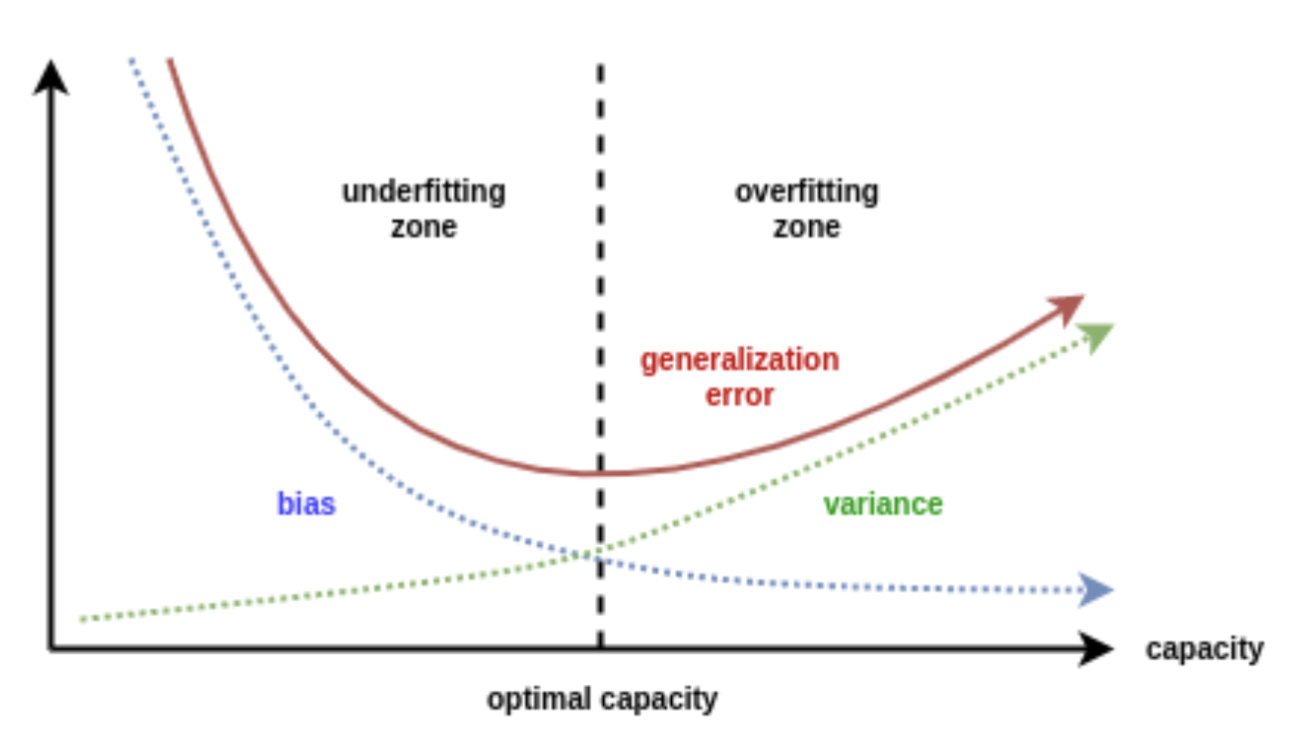
\includegraphics[width=0.6\textwidth]{images/capacity.png}
    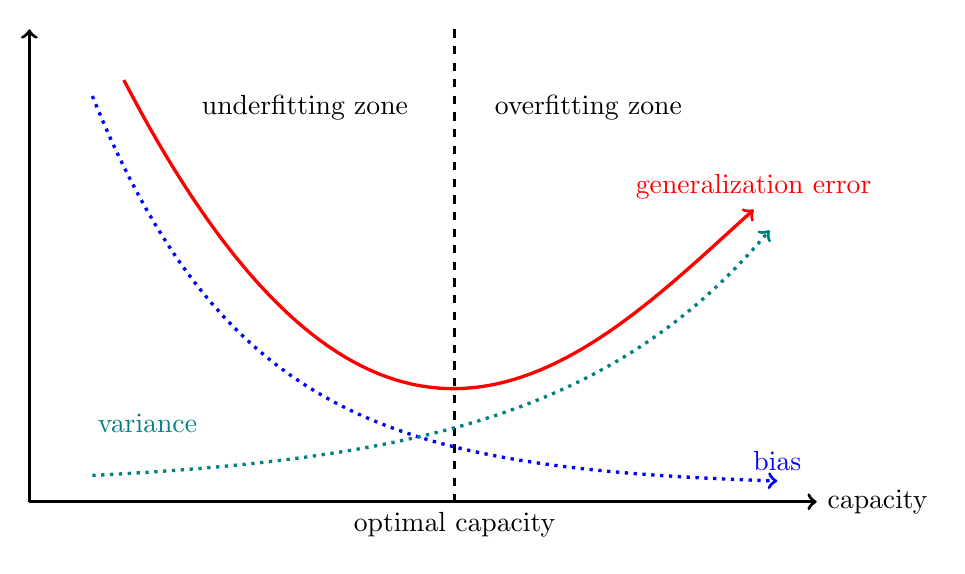
\begin{tikzpicture}[scale=1]
        \draw[->, very thick] (0,0) -- (10,0) node[right] {capacity};
        \draw[->, very thick] (0,0) -- (0,6);

        \draw[dashed, thick] (5.4, 6) -- (5.4, 0) node[below] {optimal capacity};

        \draw[->, domain=1.2:9.2, samples=75, very thick, red] plot (\x, {\x*\x*0.25-2.5*\x+25*0.25+1.8-exp(\x*0.48-3.5)}) node [above] {generalization error};
        \draw[->, domain=0.8:9.5, samples=75, very thick, blue, dotted] plot (\x, {exp(-\x*0.5+2)+0.2}) node [above] {bias};
        \draw[->, domain=0.8:9.4, samples=75, very thick, teal, dotted] plot (\x, {exp(\x*0.37-2.3)+0.2});
        \node[teal] at (1.5, 1) {variance};

        \node at (3.5, 5) {underfitting zone};
        \node at (7.1, 5) {overfitting zone};
    \end{tikzpicture}
    \caption{Effect of the capacity on bias and variance}
\end{figure}

The regime is in a regime of \emph{underfitting} when the cpacity of the hypothesis space is too small, i.e.~the chosen functions are not able to approximate well $f^*$, but at the same time there are only few functions in $\F$, the variance is therefore small.

On the other side, when we select a very large hypothesis space, there likely exists a function $f\in\F$ very close to $f^*$, inducing a small bias -- but at the same time, since $|\F|$ is big, the variance is large. 

Obviously, there are cases that are not represented by the graph above, consider for example the lucky case $\F=\{f^*\}$, or more generally $\F=\{f^*\}\cup\F_0$.

\subsubsection{Bounding the variance term: PAC bounds}
As explained above, the estimator $\hatf_n$ is a random variable. A way to deal with this randomness is to consider the expectation of $\risk(\hatf_n)$, but this is limited: it only makes statements about the risk on average. A more precise control over the excess risk can be stated in terms of a probabilistic statemet: a PAC -- Probably Approximately Correct -- bound.

\begin{definition}[$(\epsilon, \delta)$-PAC]
    We say that $\hatf_n$ is $\epsilon$-accurate with confidence $1-\delta$ of $(\epsilon, \delta)$-PAC when:
    \begin{equation}
        \P_{D_n}\left(\risk(\hatf_n) - \inf_{f\in\F}\risk(f)>\epsilon\right) < \delta
    \end{equation}
\end{definition}

Note that:
\begin{equation*}
    \risk(\hatf_n)-\inf_{f\in\F}\risk(f) = \underbrace{\left[\risk(\hatf_n)-\inf_{f\in\F}\emrisk_n(f)\right]}_{\rho_1} + \underbrace{\left[\inf_{f\in\F}\emrisk_n(f)-\inf_{f\in\F}\risk(f)\right]}_{\rho_2}
\end{equation*}

By the definition of $\hatf_n$, which is the minimum of $\emrisk_n(\hatf_n)$ over $\F$, then for the first term $\rho_1$ we have:
\begin{equation*}
    \rho_1 := \risk(\hatf_n)-\inf_{f\in\F}\emrisk_n(f) = \risk(\hatf_n)-\emrisk_n(\hatf_n) \leq \sup_{f\in\F} |\risk(f)-\emrisk_n(f)|
\end{equation*}

For the second term $\rho_2$, using the inverse triangular inequality, we have:
\begin{equation*}
    \rho_2:=\inf_{f\in\F}\emrisk_n(f)-\inf_{f\in\F}\risk(f) \leq \sup_{f\in\F}|\risk(f)-\emrisk_n(f)|
\end{equation*}

Therefore, 
\begin{equation*}
    \risk(\hatf_n)-\inf_{f\in\F}\risk(f) = \rho_1+\rho_2 \leq 2\sup_{f\in\F}|\risk(f)-\emrisk_n(f)|
\end{equation*}

\subsubsection{Bounds in probability}
In the following, we assume that $\F$ is finite and $\ell$ is bounded, that is:
\begin{equation*}
    |\F|<+\infty \quad \textnormal{and} \quad \exists M, \forall y, y'\in\Y, \:\: |\ell(y, y')|\leq M
\end{equation*}

Under these assumptions, forall $t>0$, we have by Property \ref{prop:prob-maj}:
\begin{equation*}
    \begin{aligned}
        \P\left(\risk(\hatf_n)-\inf_{f\in\F}\risk(f)>2t\right) &\leq \P\left(2\sup_{f\in\F}|\risk(f)-\emrisk_n(f)>2t\right) \\
        &\leq \sum_{f\in\F}\P\left(2\left|\risk(f)-\emrisk_n(f)\right|>2t\right) \\
        &= \sum_{f\in\F}\P\left(\left|\risk(f)-\emrisk_n(f)\right|>t\right)
    \end{aligned}
\end{equation*}
where the last step is due to Lemma \ref{lem:sup-rand-var}. To further bound the inequality above, we need to study the probability of the even $\left|\risk(f)-\emrisk_n(f)\right|>t$. Given $f\in\F$, let:
\begin{equation*}
    \forall i\in\iset{1}{n}, \quad v_i := \ell(y_i, f(x_i)) - \risk(f)
\end{equation*}
Therefore, we have:
\begin{equation*}
    \left|\emrisk_n(f)-\risk(f)\right| = \left|\frac{1}{n}\sum_{i=1}^nv_i\right|
\end{equation*}

Notice that $\E[v_i]=0$ and that the $(v_i)_i$ are independent and identically distributed. Moreover, using the assumption that $\ell$ is borned, we have that $|v_i|\leq M$ almost surely and that $\E[v_i^2]\leq M^2$. Therefore, applying the Bernstein inequality, we have:
\begin{equation*}
    \P\left(\left|\frac{1}{n}\sum_{i=1}^n v_i\right|>t\right) \leq 2\exp\left(-\frac{t^2n}{2(M^2+Mt)}\right)
\end{equation*}

Therefore, 
\begin{equation*}
    \begin{aligned}
        \P_{D_n}\left(\risk(\hatf_n)-\inf_{f\in\F}\risk(f)>2t\right) &\leq \P_{D_n}\left(2\sup_{f\in\F}\left|\risk(f)-\emrisk_n(f)\right|>2t\right) \\
        &\leq \sum_{f\in\F}\P_{D_n}\left(2\sup_{f\in\F}\left|\risk(f)-\emrisk_n(f)\right|>2t\right) \\
        &\leq \sum_{f\in\F}2\exp\left(-\frac{t^2n}{2(M^2+Mt)}\right) = 2|\F|\exp\left(-\frac{t^2n}{2(M^2+Mt)}\right)
    \end{aligned}
\end{equation*}

Now, note that when $t\leq M$, then $\exp\left(-\frac{t^2n}{2(M^2+Mt)}\right) \leq \exp\left(-\frac{t^2n}{M^2}\right)$. Let $\delta\in]0, 1[$, and when $n\leq \log \frac{2|\F|}{\delta}$, select $t=\sqrt{\frac{M^2\log \frac{2|\F|}{\delta}}{n}}$. Thus, we have $t\leq M$ and the following $(t, \delta)$-PAC bound holds:
\begin{equation*}
    \P_{D_n}\left(\risk(\hatf_n)-\inf_{f\in\R}\risk(f) > \sqrt{\frac{4M^2\log \frac{2|\F|}{\delta}}{n}}\right) \leq \delta
\end{equation*}

Equivalently, the following holds with probability at least $1-\delta$:
\begin{equation*}
    \risk(\hatf_n)-\inf_{f\in\R}\risk(f) \leq \sqrt{\frac{4M^2\log \frac{2|\F|}{\delta}}{n}}
\end{equation*}

\subsection{Bounding the Bias}
Bias term depends on the specific properties of the function $f^*$ that we try to learn, and the function space $\F$ that we have chosen. Assumptions must be done on these two objects, to quantify the bias term.

\begin{example}
    Let $\X=\R, \Y=\R$. We assume that the loss function $\ell$ satisfies the following property for some $C>0$:
    \begin{equation*}
        \forall y, y', y'', \quad |\ell(y', y)-\ell(y'', y)|\leq C|y'-y''|
    \end{equation*}
    Furthermore, we assume that the function $f^*:[-1, 1]\to\R$ can be decomposed as a power series:
    \begin{equation*}
        f^*(x) = \sum_{k=0}^{+\infty}\beta_kx^k
    \end{equation*}
    for a sequence $(\beta_k)_{k\in\N}$ such that $S:=\sum_{k=0}^{+\infty}\beta_k<+\infty$. Let $R>0$, $p\in\N$, and define:
    \begin{equation*}
        \F := \set{x\mapsto \sum_{k=1}^p\alpha_kx^k}{\alpha_k\in[-R, R]}
    \end{equation*}
    
    Denote by $f_p$ the function $f_p:x\mapsto \sum_{k=1}^p\beta_kx^k$. When $R\geq S$, $f_p\in\F$, then:
    \begin{equation*}
        \begin{aligned}
            \inf_{f\in\F}\risk(f)-\risk(f^*) \leq 
            \risk(f_p)-\risk(f^*) &= \E[\ell(f_p(x), y)-\ell(f^*(x), y)]\\
            &\leq C\cdot \E\left[\left|f_p(x)-f^*(x)\right|\right] \\
            &\leq C\cdot \E\left[\sum_{k=p+1}^{+\infty}\beta_kx^k\right] \\
            &\leq C\cdot \sum_{k=p+1}^{+\infty}|\beta^k|
        \end{aligned}
    \end{equation*}
\end{example}

%\subsection{Optional exercises}

\section{\mathpdf{k}-Nearest Neighbours}
\subsection{Introduction}
\subsubsection{Goal}
We would like to classify objects, described with vectors $x\in\R^d$, among $L+1$ classes $\Y:=\{0, \dots, L\}$, automatically. To do so, we have at hand a labelled data set of $n$ data points $(x_i, y_i)\in\R^d\times\Y$ for $i\in\iset{1}{n}$, which we assume to be the realizations of i.i.d. random variables $(X_i, Y_i)$ following a distribution $\nu$. The goal of this lesson is to build a classifier, i.e. a function
\begin{equation*}
    g:\R^d\longrightarrow\Y
\end{equation*}
which minimizes the probability of mistakes:
\begin{equation*}
    \P_{(X, Y)\sim\nu}(g(X)\neq Y) = \risk(g) := \E_{(X, Y)\sim\nu}[\ind_{g(x)\neq Y}]
\end{equation*}

\subsubsection{Intuition of the base algorithm}
The $k$-nearest neighbours classifier works as follows. Given a new input $x\in\R^d$, the classifier analyzes the $k$ nearest points $x_i$ in the data set $D_n=\set{(x_i, y_i)}{i\in\iset{1}{n}}$ and predicts a majority vote among them.

\begin{figure}[H]
    \centering
    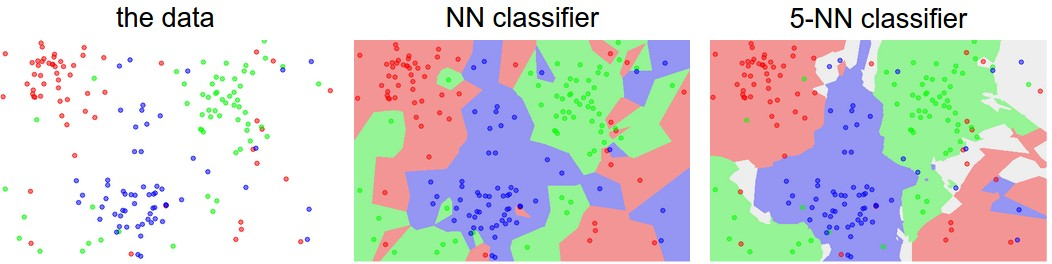
\includegraphics[width=0.8\textwidth]{images/knn.jpeg}
    \caption{$k$-NN for different values of $k$}
    \label{fig:knn}
\end{figure}

The $k$-nearest neighbor classifier is quite popular because it is simple to code and to understand; it has nice theoretical guarantess as soon as $k$ is appropriately chosen and performs reasonably well in low dimensional spaces. 

\subsubsection{Assumptions and notations}
In the following, unless stated otherwise, $\E$ and $\P$ are according to $(X, Y)\sim\nu$.

For simplicity, we will asumme in the following that we are in the binary case: $L=1$ (two classes), $\Y=\{0, 1\}$. For each $l\in\Y$, we denote by $\mu_l$ the law of $X$ given $Y$ under $\nu$ and $p_l$ the marginal distribution of $Y$:
\begin{equation*}
    \begin{cases}
        \mu_l = (X | Y=l) \\
        p_l = \P(Y=l)
    \end{cases}
\end{equation*}
We assume that $\mu_l$ is absolutely continuous with respect to Lebesgue measure on $\R^d$. We denote by $f_l$ its density, and for each $x\in\R^d$, we denote by
\begin{equation*}
    \eta(x) := \P(Y=1|X=x)
\end{equation*}

\begin{lemma}
    For any classifier $g:\R^d\longrightarrow\Y$:
    \begin{equation*}
        \risk(g) = \E[\eta(X)\cdot\ind_{g(x)=0}+(1-\eta(X))\cdot\ind_{g(X)=1}]
    \end{equation*}
    This is a simple decomposition of the risk of the classifier between the cases when $Y=1$ or $Y=0$.
\end{lemma}
\begin{proof}
    \begin{equation*}        
        \begin{aligned}
            \risk(g) &= \E[\ind_{g(X)\neq Y}]\\
            &= \E\left[\E[\ind_{g(X)\neq Y}|X]\right] \\
            &= \E\left[\E[\ind_{g(X)\neq 1}|X, Y = 1]\cdot\P(Y=1|X) + \E[\ind_{g(X)\neq Y}|X, Y=0]\cdot\P(Y=0|X)\right]\\
            &= \E\left[\E[\ind_{g(X)\neq 1}|X, Y = 1]\cdot\eta(X) + \E[\ind_{g(X)\neq Y}|X, Y=0]\cdot(1-\eta(X))\right]\\
            &= \E\left[\ind_{g(X)=0}\cdot\eta(X) + \ind_{g(X)=1}\cdot(1-\eta(X))\right]
        \end{aligned}
    \end{equation*}
\end{proof}

\subsection{Classifiers and estimators}
\subsubsection{The optimal Bayes classifier}
Notice that a random classifier sampling $g(X)=0$ and $g(X)=1$ with probability $1/2$ has an expected risk $\risk(g)=1/2$. Our goal is therefore to build a non-trivial classifier that outperforms this expected error. If the function $\eta$ was known, one could define the Bayes classifier as follows:
\begin{equation*}
    g^*(X) = \begin{cases*}
        1 & if $\eta(X)\geq1/2$\\
        0 & otherwise
    \end{cases*}
\end{equation*}

\begin{definition}[Consistency]
    We say that an estimator $\hat{g}_n$ is \emph{consistent} when:
    \begin{equation*}
        \E_{(X_i, Y_i)\sim\nu}\left[\risk(\hat{g}_n)\right] \xrightarrow[n\to+\infty]{}\risk^*
    \end{equation*}
\end{definition}

\begin{lemma}
    The risk of the Bayes classifier is
    \begin{equation*}
        \risk^* := \risk(g^*) = \E[\min(\eta(X), 1-\eta(X))]
    \end{equation*}
    Furthermore, for any classifier $g$, we have:
    \begin{equation*}
        \risk(g)-\risk^* = \E\left[|2\eta(X)-1|\cdot\ind_{g(X)\neq g^*(X)}\right] \geq 0
    \end{equation*}
    This implies that the Bayes classifier is optimal, meaning that it minimizes its risk:
    \begin{equation*}
        \risk^* = \min_{g:\R^d\to\{0, 1\}}\risk(g)
    \end{equation*}
\end{lemma}
\begin{proof}
    % TODO
\end{proof}

Therefore, if $\eta$ was known, one could compute the optimal classifier $g^*$. In practice, $\eta$ is unknown, and one should therefore estimate it.

\subsubsection{Plug-in estimator}
\begin{definition}[Estimator]
    An estimator $\hat{\eta}_n$ of $\eta$ is a function of the observation $D_n=(X_i, Y_i)_{i\in\iset{1}{n}}$ of the form:
    \begin{equation*}
        \hat{\eta}_n : \R^d \longrightarrow [0, 1]
    \end{equation*}
    where $\hat{\eta}_n$ does depend on the data set $D_n$.
\end{definition}

\begin{definition}[Plug-in estimator]
    Given an estimator $\hat{\eta}_n$ of $\eta$, we can build the \emph{plug-in estimator} as follows:
    \begin{equation}
        \hat{g}_n(x) := \begin{cases*}
            1 & if $\hat{\eta}_n(x) \geq 1/2$\\
            0 & otherwise
        \end{cases*}
    \end{equation}
\end{definition}

The intuition is that if $\hat{\eta}_n$ is close enough to $\eta$, then $\hat{g}_n$ is also close to $g^*$ and $\risk{\hat{g}_n}$ will be close to $\risk^*$. This is formalized by the following Lemma:
\begin{lemma}
    Given a plug-in estimator $\hat{g}_n$, we have:
    \begin{equation*}
        0\leq\risk(\hat{g}_n) - \risk^* \leq 2\cdot\E\left[|\eta(X)-\hat{\eta}_n(X)| \big| D_n\right]
    \end{equation*}
\end{lemma}
\begin{proof}
    % TODO
\end{proof}

This shows that for $\hat{\eta}_n = \eta$, $\hat{g}_n = g^*$, the optimal Bayes classifier. Furthermore, if $\hat{\eta}_n\simeq\eta$, then $\hat{g}_n\simeq g^*$. Therefore, if we could build from the data an estimator $\hat{\eta}_n$ of $\eta$ such that
\begin{equation*}
    \forall x\in\R^d, \quad \E\left[|\eta(X)-\hat{\eta}_n(X)| \big| D_n\right] \xrightarrow[n\to+\infty] 0
\end{equation*}
then the associated plug-in classifier would be consistent. The reverse if not true: estimating $\eta$ is harder than estimating $g^*$, since $\eta$ is real-valued while $g^*$ can only take two values. We will show that the $k$-nearest neighbors is consistent if the number of neighbors grows appropriately ($k$ is a function of $n$). This is not the case when the number of neighbors is fixed ($k$ independent of $n$).

\subsection{The \mathpdf{k}-nearest neighbors classifier (\mathpdf{k}-NN)}
The $k$-NN classifier classifies a new input $x$ with the majority class among its $k$-nearest neighbors, as can be seen in Figure \ref{fig:knn}. Formally, we denote by $\bar{X}_i(x)$ the $i$-th nearest neighbor of $x\in\R^d$ among the inputs $X_i$ (using the Euclidean distance -- that is $\ell_2$ or $\norm{\cdot}_2$). The $\bar{X}_i(x)$ are such that:
\begin{equation*}
    \norm{x-\bar{X}_1(x)}_2 \leq \norm{x-\bar{X}_2(x)}_2 \leq \dots \leq \norm{x-\bar{X}_n(x)}_2
\end{equation*}
We denote by $\bar{Y}_i(x)$ the class associated with $\bar{X}_i(x)$, which is known -- we are solving a supervised learning problem.

\begin{definition}[$k$-NN estimator]
    The estimator associated to the $k$-NN algorithm is the average of the classes among the $k$-nearest neighbors:
    \begin{equation}
        \hat{\eta}_n^k(x) := \frac{1}{k} \sum_{i=1}^k\bar{Y}_i(x)
    \end{equation}
\end{definition}

\begin{definition}[$k$-NN classifier]
    The $k$-NN classifier is the plug-in estimator associated to the $k$-NN estimator $\hat{\eta}_n^k(x)$:
    \begin{equation}
        \hat{g}_n^k(x) := \begin{cases*}
            1 & if $\frac{1}{k} \sum_{i=1}^k\bar{Y}_i(x)\geq 1/2$\\
            0 & otherwise
        \end{cases*}
    \end{equation}
\end{definition}

\begin{definition}[Asymptotic risk of the $k$-NN classifier]
    The \emph{asymptotic risk} of the $k$-NN classifier is the limit risk of $\hat{g}_n^k(x)$:
    \begin{equation*}
        \risk_{k\textnormal{-NN}} := \lim_{n\to+\infty}\E_{(X_i, Y_i)\sim\nu}[\risk(\hat{g}_n^k)]
    \end{equation*}
\end{definition}

\subsubsection{The nearest neighbor classifier (1-NN)}

\subsubsection{Inconsistency of the \mathpdf{k}-NN classifier for fixed \mathpdf{k}}

\subsubsection{Consistency of nearest neighbors making \texorpdfstring{$k\rightarrow+\infty$}{k→+∞}}

\section{Unsupervised Learning}
As described in the introduction of this course, Machine Learning is divided into three main categories: Supervised Learning, Unsupervised Learning, and Reinforcement Learning. In this chapter, we will analyze \emph{Unsupervised Learning}: while Supervised Learning provided a dataset containing both features ($x_i$) and labels ($y_i$); in Unsupervised Learning, the dataset contains only features $x_i$.

\subsection{\mathpdf{K}-means}
$K$-means clustering is a method of vector quantization. $K$-means clustering is an algorithm of alternate minimization that aims at partitioning $n$ observations into $K$ clusters in which each observation belongs to the cluster with the nearest mean, serving as a prototype to the cluster.


\subsubsection{Distortion}
\begin{definition}[Observations]
    In the clustering problem, we are given $x_i\in\R^p$ for $i\in\iset{1}{n}$, the \emph{observations} we want to partition.
\end{definition}

\begin{definition}[Means]
    For some given $K$, we denote $\mu_k\in\R^p$ for $k\in\iset{1}{K}$ the means. $\mu_k$ is the center of the cluster $k$. We will denote $\mu$ the associated matrix.
\end{definition}

\begin{definition}[Hard membership variables]
    $z_i^k\in\{0, 1\}$ are indicator variables associated to $x_i$, such that:
    \begin{equation*}
        z_i^k := \begin{cases*}
            1 & if $x_i$ belongs to the cluster $k$\\
            0 & otherwise
        \end{cases*}
    \end{equation*}
    We denote by $z$ the matrix which components are equal to $z_i^k$.
\end{definition}

\begin{definition}[Distortion]
    We define the distortion $J(\mu, z)$ by:
    \begin{equation}
        J(\mu, z) := \sum_{i=1}^n \sum_{k=1}^K z_i^k \norm{x_i-\mu_k}^2
    \end{equation}
    Distortion measures the overall distance of the centers $\mu_k$ to the points of the cluster.
\end{definition}

\begin{definition}[$K$-means optimization problem]
    The \emph{$K$-means optimization problem} consists in finding matrices $\mu$ and $z$ which minimize the distortion:
    \begin{equation}
        \min_{\substack{\mu\in\mathscr{M}_{n, k}(\R)\\z\in\mathscr{M}_{n, k}(\R)}} J(\mu, z) = \min_{\substack{\mu\in\mathscr{M}_{n, k}(\R)\\z\in\mathscr{M}_{n, k}(\R)}} \sum_{i=1}^n \sum_{k=1}^K z_i^k \norm{x_i-\mu_k}^2
    \end{equation}
\end{definition}

\subsubsection{Algorithm}
To minimize $J(\mu, z)$, we proceed using an alternating minimization: we will minimize $J$ alternatively with respect to $z$ and $\mu$.

\begin{enumerate}
    \item Randomly choose a vector $\mu$.
    \item Minimize $J$ with respect to $z$:
    \begin{equation}
        z_i^k = \begin{cases*}
            1 & if $\norm{x_i-\mu_k}^2 = \min_s \norm{x_i-\mu_s}^2$\\
            0 & otherwise
        \end{cases*}
    \end{equation}
    This is equivalent to associating to $x_i$ the nearest center $\mu_k$.
    \item Minmize $J$ with respect to $\mu$:
    \begin{equation}
        \label{eq:minimize-mu}
        \mu_k = \frac{\sum_{i=1}^n z_i^k x_i}{\sum_{i=1}^n z_i^k}
    \end{equation}
    \item Come back to step 2 until convergence.
\end{enumerate}

\begin{proof}
    The formula \eqref{eq:minimize-mu} can be obtained by minmizing the gradient of $J$ with respect to $\mu_k$:
    \begin{equation*}
        \nabla_{\mu_k} J = -2 \sum_{i=1}^n z_i^k (x_i-\mu_k)
    \end{equation*}
    Therefore:
    \begin{equation*}
        \nabla_{\mu_k} J = 0 \iff \mu_k = \frac{\sum_{i=1}^n z_i^k x_i}{\sum_{i=1}^n z_i^k}
    \end{equation*}
\end{proof}

\subsubsection{Convergence and initialization: \mathpdf{K}-means++}
We can show that this algorithm converges in a finite number of iterations. Nevertheless, the convergence could be towards to local minimum, introducing the problem of initialization.

A classic method is to use random restarts. It consists in choosing serveral random vectors $\mu$, computing the algorithm for each case and finally keeping the partition wihch minimizes the distortion. Thus, we hope that at least one of the local minima is close enought to a global minimum.

Another well known method is the $K$-means++ algorithm, which aims at correcting a major theoretical shortcoming of the $K$-means algorithm: the approximation found can be arbitrarily bad with respect to the objective function compared to the optimal clustering.

The $K$-means++ algorithm addresses this obstacles by specifying a procedure to initialize the cluster centers before proceeding with the standard $K$-means optimization iterations. With the $K$-means++ initialization, the algorithm is guaranteed to find a solution that is $O(\log K)$ competitive to the optimal $K$-means solution.

The intuition behind this approach is that spreading the $K$ initial cluster centers will improve the quality of the clusters found by the algorithm. At each iteration of the algorithm we will build a new center, and repeat this step until we have $K$ centers. Here are the steps of the algorithm:
\begin{enumerate}
    \item Choose the first center uniformly among the data points.
    \item For each data point $x_i$ of the data set, compute the distance between $x_i$ and the nearest center that has already been chosen. We denote this distance $D_{\mu_t}(x_i)$ where $\mu_t$ is specified to recall that we are minimizing over the current chosen centers.
    \item Choose a new data point at random as a new center, but now using a weighted probability distribution where a point $x_i$ is chosen with probability proportional to $D_{\mu_t}(x_i)^2$.
    \item Come back to step 2 until $K$ centers have been chosen.
\end{enumerate}

We see that we have now built $K$ vectors with respect to our first intuition which was to well spread the centers -- because we used a well-chosen weighted probability. We can now use those vectors as the initialization of our standard $K$-means algorithm.

\subsubsection{Choice of \mathpdf{K}}
It is important to point out that the choice of $K$ is not universal. Indeed, we see that if we increase $K$, the distortion $J$ decreases, until reaches $0$ when $K=n$ --  when each data point is the center of its own cluster. To address this issue, one solution could be to add to $J$ a penalty over $K$. Usually, it takes the following form:
\begin{equation*}
    J(\mu, z, K) := \sum_{i=1}^n\sum_{k=1}^K z_i^k\norm{x_i-\mu_k}^2+\lambda K
\end{equation*}
Once again, the choice of the penalty coefficient $\lambda$ is arbritrary. There is no general way to choose $K$.

\subsubsection{Other problems}
We can also point out that $K$-means will work properly when the width of the different clusters are similar -- for example when dealing with spheres. But clustering by $K$-means could also be disappointing in some cases such as the following example:
\begin{figure}[H]
    \centering
    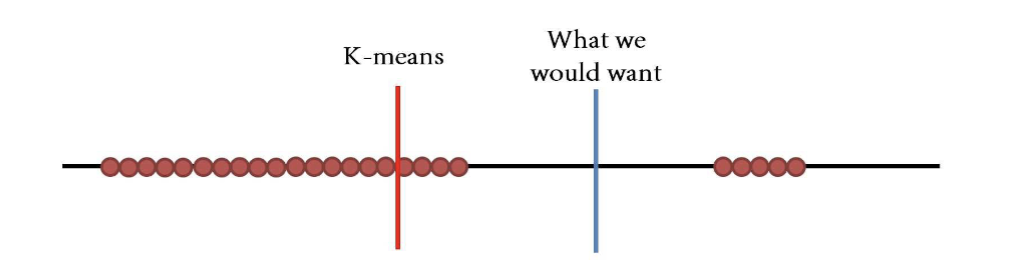
\includegraphics[width=0.7\textwidth]{images/k-means-limitations.png}
    \caption{Example where $K$-means does not provide a satisfactory clustering result}
\end{figure}
For instance, the use of Gaussian mixtures provides a way to avoid this problem.

\subsection{Dimensionality reduction: principal component analysis}
Imagine that we want to process some video data $(x_i)_{i\in\iset{1}{n}}$ where $x_i\in\R^p$. In the case of video data, $p$ can be prohibitively huge to manipulate, e.g. $p\simeq10^{11}$. We would like to reduce the dimensionality of the origin space, i.e. finding a new representation for each of the $x_i$:
\begin{equation*}
    x_i\in\R^p \longmapsto \hat{x}_i\in\R^{p'} \where p' \ll p
\end{equation*}
without loosing too much information.

\begin{figure}[H]
    \centering
    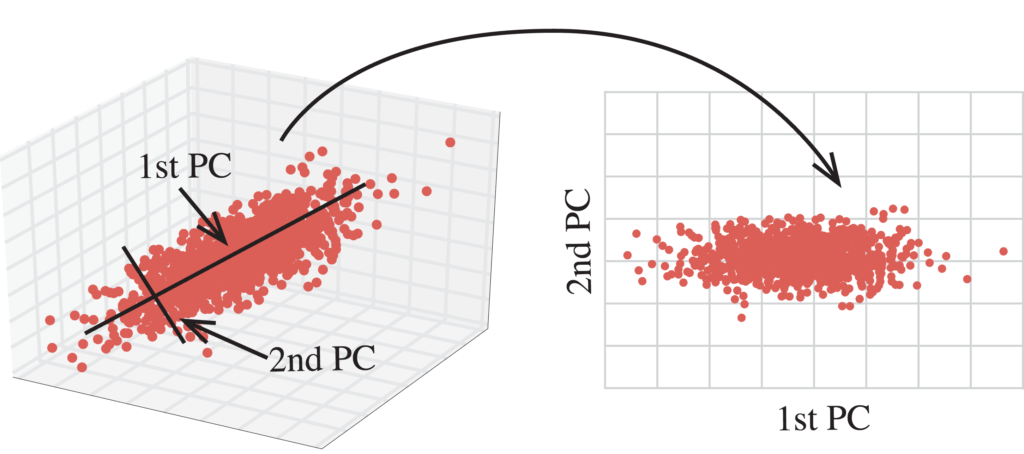
\includegraphics[width=0.7\textwidth]{images/dimensionality-reduction.png}
    \caption{Dimensionality reduction from $\R^3$ to $\R^2$, i.e. using two principal components}
\end{figure}

\subsubsection{Analysis view}
We will start by introducing formally the problem. Assume that there is some data distribution $\nu$ over $\R^p$. A random variable $X\in\R^p\sim\nu$ samples this data distribution over this high-dimensional space. Assume that $\E[X]=0$, and let
\begin{equation*}
    \Sigma:=\Cov(X)=\E\left[(X-\E[X])(X-\E[X])^\tp\right]=\E[XX^\tp]
\end{equation*}
$\Sigma$ is the covariance matrix of $X$; note that it is definite non-negative.

The intuition is that we want to preserve as much \say{diversity} in the output after the dimension reduction. This leads to the following definition of the problem in the case where $p'=1$.
\begin{definition}[PCA problem]
    Find $w\in\R^{p}$ such that:
    \begin{equation}
        \label{eq:pca-problem}
        w\in\argmax_{\norm{w}=1}\V(w^\tp X)
    \end{equation}
\end{definition}

\begin{theorem}
    $w$ verifies \eqref{eq:pca-problem} exactly when $w$ is the eigenvector of $\Sigma$ corresponding to the largest eigenvalue.
\end{theorem}
\begin{proof}
    Note that:
    \begin{equation*}
        \begin{aligned}
            \V(\omega^\tp X)&=\E[\omega^\tp X]^2-(\E[\omega^\tp X])^2\\
            &= \E[(\omega^\tp X)(\omega^\tp X)] \\
            &= \E[\omega^\tp XX^\tp\omega]\\
            &=\omega^\tp\E[XX^\tp]\,\omega \\
            &= \omega^\tp\Sigma\,\omega
        \end{aligned}
    \end{equation*}
    Therefore,
    \begin{equation*}
        \sup_{\norm{\omega}=1}\V(\omega^\tp X) = \sup_{\norm{\omega}=1}\omega^\tp\Sigma\,\omega
    \end{equation*}
    Thus, by property, $\omega$ is exactly the eigenvector of $\Sigma$ corresponding to the largest eigenvalue. We can write $\Sigma=UDU^\tp$ with $U\in\R^{p\times p}$, and $UU^\tp=I_p$, with $D=\diag(\lambda_1, \dots, \lambda_p)$. If we assume $\lambda_1\geq\dots\geq\lambda_p$, we have that $\omega$ is the first column of $U$. %(cf. photo)
\end{proof}

\begin{remark}
    To generalize this procedure to $p'$ dimensions, we take the $p'$ eigenvectors associated to the $p'$ largest eigenvalues. Another approach would be to use \emph{deflation}, defined by the following algorithm:
    \begin{enumerate}
        \item Find $w$ using the largest eigenvalue.
        \item Project the data onto $\Span(w)$.
        \item Start at Step 1.
    \end{enumerate}
\end{remark}

\subsubsection{In practice}
In practice, we do not know $\Sigma$ -- since it depends on the unknown distribution $\nu$ -- but we are given a dataset to work with. Given $(x_i)_{i\in\iset{1}{n}}$, we want to find a vector $w\in\R^p$ -- or a matrix $W\in\mathscr{M}_{p, p'}(\R)$ -- such that the associated projection maximizes the variance of the projected dataset. In the theoretical analysis, we assumed that $\E[X]=0$; to verify the assumptions, we need the dataset to be centered, or \emph{center} it if necessary. Thus, we introduce the mean of the dataset (a vector) and substract it to the initial dataset:
\begin{equation*}
    x_i\leftarrow x_i-\mu \where \mu=\frac{1}{n}\sum_{i=1}^n x_i
\end{equation*}

This being done, we can define the \emph{empirical covariance matrix}, which is the approximation of the covariance matrix $X$ with respect to the dataset available:
\begin{equation*}
    \hat{\Sigma} := \frac{1}{n} \sum_{i=1}^n  x_ix_i^\tp
\end{equation*}
Similarly to the theoretical setting, we can use the normlized eigenvectors associated to the largest eigenvalues to construct a matrix maximizing the variance.

\section{Probabilistic models and Maximum Likelihood}
\subsection{Introduction}
In probabilistic modeling, we are given a set of observations $D_n=(y_1, \dots, y_n)$ in $\Y$ that we assume to be generated from some unknown i.i.d.~distribution. As always, the objective is to find a probabilistic model that explains well the data, by estimating the density of the underlying distribution. If possible, we would like the model to predict well new data and to be able to incorporate prior knowledge and assumptions.

Let $\mu$ denote some reference measure on the output set $\Y$. Typically, $\mu$ is the counting measure if $\Y\subseteq\N$ or the Lebesgue measure if $\Y\subseteq\R^d$.

\begin{definition}[Parametric model]
    Let $d\geq1$ and $\Theta\subseteq\R^d$ by a set of parameters. A parametric model $\Pc$ is a set of probability distributions taking value in $\Y$ with a density with respect to $\mu$ and indexed by $\Theta$:
    \begin{equation}
        \Pc = \set{p_\theta\dd\mu}{\theta\in\Theta}
    \end{equation}
\end{definition}

Here are a few examples of statistical parametric models based on well known family distributions.
\begin{example}[Binomial model]
    For $\Y=\N$ and $\Theta=[0, 1]$:
    \begin{equation*}
        p_\theta(k) = \binom{n}{k}\theta^k(1-\theta)^{n-k}
    \end{equation*}
\end{example}

\begin{example}[Gaussian model]
    For $\Y=\R$ and $\Theta=\R\times\R_+$, where we traditionnaly denote elements of $\Theta$ as $(\mu, \sigma)$, the parameters of the normal distribution:
    \begin{equation*}
        p_{(\mu, \sigma)}(x) = \frac{1}{\sqrt{2\pi}\sigma} \exp\left(-\frac{(x-\mu)^2}{2\sigma^2}\right)
    \end{equation*}
\end{example}

\begin{example}[Multidimensional\footnote{Also known as \emph{multivariate}.} Gaussian model]
    For $\Y=\R$ and $\Theta=\R^d\times S_d^+(\R)$\footnote{$S_d^+(\R)$ denotes the set of semi-definite positive matrices. In particular, such matrices $M$ are invertible, and the associated bilinear form is positive: $\forall x\in\R^d, x^\tp Mx$.}, where we traditionnaly denote elements of $\Theta$ as $(\mu, \Sigma)$, the parameters of the normal distribution:
    \begin{equation*}
        p_{(\mu, \Sigma)}(x) = \frac{1}{(2\pi)^{d/2}|\Sigma|^{1/2}} \exp\left(-\frac{1}{2}(x-\mu)^\tp\Sigma^{-1}(x-\mu)\right)
    \end{equation*}
\end{example}
Other parametric models include the \href{https://en.wikipedia.org/wiki/Exponential_distribution}{exponential model} on $\Y=\R_+$, the \href{https://en.wikipedia.org/wiki/Bernoulli_distribution}{Bernoulli model} on $\Y=\{0, 1\}$, \dots

In the following, we assume that we are given some model $\Pc$ indexed by $\theta\in\Theta$, and we assume that the data $D_n$ is independently generated from $p_{\theta_*}\in\Pc$ for some unknown parameter $\theta_*$. We would like to recover the best parameter $\theta_*$ from the data. 

\begin{remark}
    In practice, the data might come from a distribution which is not in $\Pc$: this is called misspecification, but we will not enter into further details in this chapter.
\end{remark}

\subsection{Maximum likelihood estimation}
\subsubsection{Definition and example}
The idea behind maximum likelihood estimation is to choose the most probable parameter $\theta\in\Theta$ for the observed data. Assume that $\Y$ is discrete and that $Y\sim p_{\theta_*}\dd\mu$ for some $\theta_*\in\Theta$. Then, for any observation $y_i$, the probability that $Y=y_i$ equals $p_{\theta_*}(y_i)$:
\begin{equation*}
    \P(Y=y_i) = p_{\theta_*}(y_i)
\end{equation*}
Similarly, the probability of observering $(y_1, \dots, y_n)\in\Y^n$ if all the samples were independently sampled from $p_\theta$ is $\prod_{i=1}^m p_\theta(y_i)$. Hence, the high level idea of maximum likelihood estimation will be to maximize this probability over $\theta\in\Theta$. This is formalized by the definition of the likelihood, which also holds for non-discret set $\Y$.

\begin{definition}[Likelihood]
    Let $\Pc = \set{p_\theta\dd\mu}{\theta\in\Theta}$ be a parametric model and $y\in\Y$. Given the outcome $y\in\Y$, the \emph{likelihood} is the function:
    \begin{equation}
        \theta \longmapsto p_\theta(y)
    \end{equation}
    The likelihood $L(\cdot|D_n)$ of a dataset $D_n=(y_1, \dots, y_n)$ is the function:
    \begin{equation}
        L(\cdot|D_n) : \theta \longmapsto \prod_{i=1}^m p_\theta(y_i)
    \end{equation}
\end{definition}

\begin{definition}[Maximum likelihood estimator]
    The \emph{maximum likelihood estimator (MLE)} is the parameter which maximizes the likelihood, i.e.:
    \begin{equation}
        \htheta_n\in\argmax_{\theta\in\Theta} \prod_{i=1}^n p_\theta(y_i)
    \end{equation}
\end{definition}

In practice, maximizing a sum is easier than to maximize a product. Since $\log$ is an increasing function, the maximum likelihood estimator also maximizes the \emph{$\log$-likelihood}:
\begin{equation}
    \htheta_n\in\argmax_{\theta\in\Theta} \sum_{i=1}^n \log p_\theta(y_i)
\end{equation}

\begin{example}[Bernoulli model]
    For $\Y=\{0, 1\}$ and $\Theta=[0, 1]$, we define the Bernoulli model as:
    \begin{equation*}
        p_\theta(y) = \theta^y(1-\theta)^{(1-y)}
    \end{equation*}
    Assuming that $D_n$ was generated from a Bernoulli distribution of parameter $\theta_*$; then, the maximum likelihood estimator is:
    \begin{equation*}
        \htheta_n\in\argmin_{0\leq\theta\leq1} \frac{1}{n} \sum_{i=1}^n \left[y_i\log\theta + (1-y_i)\log(1-\theta)\right]
    \end{equation*}
    Denoting $\bar{y}_n := \sum_{i=1}^ny_i$ the empirical average, we solve:
    \begin{equation*}
        \frac{\dd\log L(\theta|D_n)}{\dd\theta} \biggr\rvert_{\theta=\htheta_n} = 0 \implies \frac{\bar{y}_n}{\htheta_n} - \frac{1-\bar{y}_n}{1-\htheta_n} \implies \htheta_n = \bar{y}_n
    \end{equation*} 
    Therefore, the maximum likelihood estimator is in this case the empirical mean.
\end{example}

\subsubsection{Link with empirical risk minimization}
In this chapter, we studied density estimation, in which the goal is to find the density of the distribution which generated the data. This can be connected to empirical risk minimization: assuming that the density belongs to the model $\Pc$, the possible densities are $p_\theta$, for some $\theta\in\Theta$. We can define a loss function for this setting to be the negative log-likelihood:
\begin{equation}
    \begin{aligned}
        \ell : \Theta\times\Y &\longrightarrow \R^+ \\
        (\theta, y) &\longmapsto -\log p_\theta(y)
    \end{aligned}
\end{equation}
The risk -- or generalization error -- is then:
\begin{equation}
    \risk(\theta) = - \E_Y\left[\log p_\theta(Y)\right]
\end{equation}

In particular, if $Y\sim p_{\theta_*}\dd\mu$, for some $\theta_*\in\Theta$, $\theta_*$ minimizes the risk and the objective is to recover $\theta_*$. The empirical risk is then, by definition:
\begin{equation}
    \hat{\risk}_n(\theta) = -\frac{1}{n}\sum_{i=1}^n \log p_\theta(y_i)
\end{equation}

Therefore, the empirical risk minimizer matches the maximum likelihood estimator.

\subsubsection{Link with Kullback-Leibler divergence}
The Kullback-Leibler divergence is a measure of dissimilarity between two probability distributions.

\begin{definition}
    Let $p\dd\mu$ and $q\dd\mu$ be two probability distributions with $p\ll q$\footnote{We say that $q$ is \emph{absolutely continuous with respect to $p$}, meaning that $q(A)=0\implies p(A)=0$}. The \emph{Kullback-Leibler divergence from $q$ to $q$} is defined as:
    \begin{equation}
        \KL(p||q) := \E_{Y\sim p\dd\mu} \left[\log\frac{p(Y)}{q(Y)}\right] = \int_{\Y}p(y)\log\frac{p(y)}{q(y)}\dd\mu(y)
    \end{equation}
\end{definition}

The Kullback-Leibler divergence has two interpretations. In information theorey, it can be seen as the difference of symbols needed to encode $D_n$ under a code optimized for $p\dd\mu$ compared to a code optimized for $q\dd\mu$. 

$\KL(p_\theta||p_{\theta_*})$ can also be interpreted as the excess risk of the measure $p_\theta\dd\mu$ when the data follows distribution $p_{\theta_*}\dd\mu$ for the negative log-likelihood loss function. Assume that the data $D_n$ was generated form $p_\theta$. Then, the excess risk can be written:
\begin{equation*}
    \begin{aligned}
        \risk(\theta)-\risk(\theta_*) &= -\E_{Y\sim p_{\theta_*}\dd\mu}\left[\log p_\theta(Y)\right] + \E_{Y\sim p_{\theta_*}\dd\mu}\left[\log p_{\theta_*}(Y)\right]\\
        &= \E_{Y\sim p_{\theta_*}\dd\mu}\left[\log \frac{p_{\theta_*}(Y)}{p_\theta(Y)}\right]\\
        &=: \KL(p_{\theta_*}||p_\theta)
    \end{aligned}
\end{equation*}

\begin{property}[Positivity]
    By Jensen's inequality:
    \begin{equation}
        \KL(p||q) \geq 0
    \end{equation}    
\end{property}

\begin{property}[Separation]
    \begin{equation}
        \KL(p||p) = 0
    \end{equation}
    Therefore, $p_{\theta_*}$ minimizes the risk and maximizes the likelihood.
\end{property}

\begin{property}[Discrete case]
    If $\Y$ is discrete and $\mu$ is the counting measure, we have:
    \begin{equation}
        \KL(p||q) = \sum_{y\in\Y}p(y)\log\frac{p(y)}{q(y)}
    \end{equation}
\end{property}

Note that the KL divergence is often seen as a distance, but it does fill the requirements, since it is not symmetric and does not satisfy the triangular inequality.

\subsubsection{Conditional modeling}
Until now, we considered the problem of density estimation when the data set has only outputs $y_i\in\Y$. Howerver, the principle of maximum likelihood can be extended to couples of inputs $D_n=\{(x_1, y_1), \dots, (x_n, y_n)\}\in\X\times\Y$. Then, we can distinguish two different modeling: generative and conditional modeling.

\paragraph*{Generative modeling}
We aim at estimating the density of couples of input and ouputs $(X, Y)$ among a family of densities on $\X\times\Y$:
\begin{equation*}
    (x, y) \longmapsto p_\theta(x, y)
\end{equation*}
In this case, the risk and the empirical risk are:
\begin{equation*}
    \begin{cases}
        \risk(\theta)=-\E[\log p_\theta(X, Y)]\\
        \emrisk_n(\theta) = -\frac{1}{n}\sum_{i=1}^n\log p_\theta(x_i, y_i)
    \end{cases}
\end{equation*}
Estimating the density can be useful to generate some new samples.

\paragraph*{Conditional modeling}
We aim at estimating the density of an ouput $Y$ \emph{given $X$}. The densities now are on $\Y$ only:
\begin{equation*}
    y \longmapsto p_\theta(\cdot|x)
\end{equation*}
but do depend on the inputs. The risk and the empirical risk with negative log-likelihood are:
\begin{equation*}
    \begin{cases}
        \risk(\theta)=-\E[\log p_\theta(Y|X)]\\
        \emrisk_n(\theta) = -\frac{1}{n}\sum_{i=1}^n\log p_\theta(y_i|x_i)
    \end{cases}
\end{equation*}
This is useful if one wants to predict the distribution or the value of a new ouput $Y$ given an input $X$.

\subsubsection{Linear regression as conditional modeling}
Unlike Hinge loss, logistic loss has a probabilist interpretaton. Consider $(X, Y)\sim\Pc$ a pair of input-output random variables in $\R^d\times\{0, 1\}$. In binary classification, the objective is to predict the probability that $Y=1$ given the input $X$. In other words, we want to estimate $\P(Y=1|X)$, that is:
\begin{equation*}
    x \longmapsto \P(Y=1|X=x)
\end{equation*}
from observations $D_n=\set{(x_i, y_i)}{i\in\iset{1}{n}}\subseteq\R^d\times\{0, 1\}$, that were independently generated from $\Pc$. The issue is that linear predictions of the form $\theta^\tp x_i$ belong to $\R$, while our model needs to output probabilities with values in the range $[0, 1]$. Therefore, the \emph{sigmoid} function is often used, which maps $\R$ to $[0, 1]$.

\begin{definition}[Sigmoid function]
    The sigmoid function $\sigma$ is defined by:
    \begin{equation}
        \begin{aligned}
            \sigma : \R &\longrightarrow [0, 1]\\
            z &\longmapsto \frac{1}{1+e^{-z}}
        \end{aligned}
    \end{equation}
\end{definition}

\begin{property}
    The following identity holds: $\sigma(-z)=1-\sigma(z)$
\end{property}

\begin{property}[Derivative of sigmoid]
    The derivative of sigmoid is: $\sigma'(z)=\sigma(z)\sigma(-z)$
\end{property}

Logistic regression assumes the underlying probabilistic model:
\begin{equation*}
    \P(Y=1|X)=\sigma(\theta^\tp X)
\end{equation*}
It is worth pointing out that this probabilistic model is satisfied for many natural models: for instance, if $X|Y=1$ and $X|Y=0$ follow independent Gaussian distributions, this model is satsfied.

We can define the family of possible densities (with respect to the countable measure) on $\{0, 1\}$ considered here:
\begin{equation}
    \label{eq:parametric-model}
    p_\theta(y|x) = \sigma(\theta^\tp x)^y\left(1-\sigma(\theta^\tp x)\right)^{1-y} = \begin{cases*}
        1-\sigma(\theta^\tp x) & if $y=0$\\
        \sigma(\theta^\tp x) & otherwise
    \end{cases*}
\end{equation}
indexed by $\theta\in\R^d$. We recall that similarly to linear regression, to ease the notation, the intercept (to make affine predictions) may be included into the input $X$ by adding the constant 1 as the first coefficient.

\begin{property}
    Assume that the $(x_i, y_i)$ are realizations of i.i.d.~random variables. Then, the logistic regression estimator \begin{equation*}
        \htheta \in\argmin_{\theta\in\R^d} \sum_{i=1}^n \ell(\theta^\tp x_i, y_i) \where \ell(x, y) := y\log\sigma(x) + (1-y)\log\sigma(-x)
    \end{equation*}
    matches the definition of the maximum likelihood estimator of $\theta\in\R^d$ with parametric model \eqref{eq:parametric-model}.
\end{property}

\begin{proof}
    The conditional log-likelihood can be written:
    \begin{equation*}
        \begin{aligned}
            \log L(\cdot|D_n) &= \sum_{i=1}^n \log p_\theta(y_i|x_i)\\
            &= \sum_{i=1}^n \log\left(\sigma(\theta^\tp x)^y\left(1-\sigma(\theta^\tp x)\right)^{1-y}\right)\\
            &= \sum_{i=1}^n y\log\left(\sigma(\theta^\tp x)\right) + (1-y)\log\left(1-\sigma(\theta^\tp x)\right)\\
            &= \sum_{i=1}^n \ell(\theta^\tp x_i, y_i)
        \end{aligned}
    \end{equation*}
    where $\ell$ is the logistic loss defined above.
\end{proof}

\subsection{Maximum a posteriori}
If the dimension $d$ of the parameter space $\Theta$ is too large compared to the number of samples $n$, the maximum likelihood estimator (MLE) may lead to poor performance. Similarly to least square linear regression without regularization, MLE overfits when $d>n$. A second limitation is that no prior knowledge on the parameters $\theta$ is included. Let us detail this using an example.

\begin{example}
    We consider the multinomial model where each observation is a discrete observation in $k$ classes $\{1, \dots, k\}$. Each class $j\in\{1, \dots, k\}$ is samples with a probability $\theta^*_j$, and we aim at retrieving these probabilities. We define for convenience the output set:
    \begin{equation*}
        \Y=\set{y\in\{0, 1\}^k}{\sum_{i=1}^ky_i=1}
    \end{equation*}
    An observation $y$ is sucht that $y(j)=1$ if it is in class $j\in\{1, \dots, k\}$, and 0 otherwise. The multinomial model consists of densities of the form:
    \begin{equation*}
        p_\theta : y\in\Y\longmapsto\prod_{j=1}^k\theta_j^{y(j)} \where \theta\in[0, 1]^k, \quad \sum_{j=1}^k\theta_j=1
    \end{equation*} 
    In other words, the probability of an observation to be in class $j$ equals $\theta_j$, since only one term of the product is different from 1. The dimension of the parameter space is $d=k-1$ --  we choose $k$ coefficients for $\theta$, with 1 constraint. The MLE is:
    \begin{equation*}
        \htheta_j = \argmax_{\theta_j} \frac{1}{n}\sum_{i=1}^n y_i(j)\log\theta_j = \frac{n_j}{n} \where n_j = \sum_{i=1}^n y_i(j)
    \end{equation*}
    $n_j$ is the number of occurence of class $j$ in the data set. If $k>n$, many classes $j$ are never observed and estimated with 0. This can happen, for example, when we are trying to associate probabilities to words, each word being its own class, but the number of possible words $k$ is much larger than the number of words in the dataset text. The log-loss of these options is infinite, and so is the risk $\risk(\theta)$. We say that the model is overestimating.
\end{example}

This problem can be solved by adding a regularization, which can also be seen from a Bayesian point of view as a prior distribution over the possible distributions $\theta$. This is what Maximum a Posteriori (MAP) does. The idea behind MAP is to see the parameter $\theta$ as a random variable taking values in $\Theta$, and to choose the most probable value $\htheta^{\textnormal{MAP}}$ for the observed data. Given the data set $D_n$, the MAP can be formalized as the solution of:
\begin{equation*}
    \htheta_n^{\textnormal{MAP}}\in\argmax_{\theta\in\Theta}p(\theta|D_n)
\end{equation*}
where $p(\theta|D_n)$ is the density of the posterior distribution of the model given the data. In discrete model space $\Theta$, the MAP is exactly the most probable model. To calculate the posterior distribution we use the Bayes rule:
\begin{equation*}
    p(\theta|D_n) = \frac{p(D_n|\theta)\cdot p(\theta)}{p(D_n)}
\end{equation*}
where:
\begin{itemize}
    \item $D_n$ is a random data set
    \item $p(D_n|\theta)$ is the probability density of observing $D_n$ is the distribution follows $p_\theta\dd\mu$. This is exactly the likelihood $L(\theta|D_n)$
    \item $p(\theta)$ is the prior distribution of the model, that this how likely we think it is before seeing the data
    \item $p(D_n)$ is the marginal distribution of the data
\end{itemize}

Hence, the MAP is the solution of:
\begin{equation}
    \htheta_n^{\textnormal{MAP}} \in \argmax_{\theta\in\Theta} L(\theta|D_n)\cdot p(\theta) = \argmin_{\theta\in\Theta} -\frac{1}{n}\sum_{i=1}^n\log p_\theta(y_i) + \log\frac{1}{p(\theta)}
\end{equation}
In some situation, we may not have to prefer one model over another, and one can think of $p(\theta)$ as a constant of the parameter space $\Theta$. Then, the MAP with uniform prior reduces to the MLE. However, this assumption that $p(\theta)$ is constant is problematic, because uniform distribution cannot always be defined if $\Theta$ is not compact. Therefore, it may be better to see MAP as a regularized version of MLE, with a regularization of the form $-\log p(\theta)$, rather than MLE as a particular case of MAP with uniform prior.

\section{Posterior sampling using MCMC and SGLD}
So far, we have discussed several tasks that arise in statistical learning, and we expressed most of these tasks by certain optimization problems, such as the empirical risk minimization problem. The Maximum A Posteriori (MAP) estimation problem, introduced in the previous chapter, being one of the examples of such optimization problems, arose natuarally when we limited ourselves to the framework of probabilistic modeling. In this chapter, we will again consider the probabilistic modeling framework, but this time with a different question than the MAP estimation problem.

\subsection{Introduction}
\subsubsection{Bayesian probabilistic model}
Let's start by remembering what a Bayesian probabilistic model is. The main idea in Bayesian modeling is to treat the parameter of interest $\theta\in\R^d$ as a random vector that follows a \emph{prior distribution} $p(\theta)$. 

A single observation $y$ is assumed to be a random variable drawn from the \emph{conditional distribution} $p(y|\theta)$. We typically consider $n$ observations $D_n=\{y_1, \dots, y_n\}$, which are i.i.d.~distributed when conditioned on $\theta$. 

We often denote a Bayesian probabilistic model as follows:
\begin{equation}
    \begin{aligned}
        \theta&\sim p(\theta)\\
        \forall i\in\iset{1}{n}, \quad y_i|\theta&\sim p(y|\theta)
    \end{aligned}
\end{equation}
Under this model, the goal in MAP estimation is to find the value $\htheta_n$ that maximizes the \emph{posterior distribution}:
\begin{equation}
    p(\theta|D_n) = \frac{p(D_n|\theta)p(\theta)}{p(D_n)}
\end{equation}

Since the logarithm function is monotonic and $p(D_n)$ does not depend on $\theta$, the MAP estimation problem can be written in the following form:
\begin{equation}
    \htheta_n\in\argmax_\theta \sum_{i=1}^n\log p(y_i|\theta)+\log p(\theta)
\end{equation}

\subsubsection{Level of uncertainty}
The MAP estimator can be very useful in practical applications and there is a broad literature for solving this optimization problem for a variety of choices of prior distributions, with various theoretical guarantees. However, in a broad range of applications, a single point estimate can be insufficient, especially for risk-intolerant applications (such as autonomous driving). Hence, it would be of interest to extract more information about our estimate to have an understanding of \emph{the level of uncertainty} in our estimation.

While there are many ways of doing this, here, we will consider the Bayesian approach and try to infer the uncertainty information by making a better use of the posterior distribution. For instance, as a measure of uncertainty, we can consider the posterior variance.

\begin{definition}[Posterior variance]
    The \emph{posterior variance}, denoted $\sigma^2_{\textnormal{post}}$, is defined by:
    \begin{equation}
        \sigma^2_{\textnormal{post}} := \int\norm{\theta-\mu_{\textnormal{post}}}^2 \cdot p(\theta|D_n)\dd\theta 
        \where \mu_{\textnormal{post}} := \int \theta\cdot p(\theta|D_n)\dd\theta
    \end{equation}
    Note that $\mu_{\textnormal{post}}$ is the posterior expectation. Intuitively, if the value of $\sigma^2_{\textnormal{post}}$ is high, we might conclude that there is a high uncertainty in our estimation: the posterior distribution is too widespread. If $\sigma^2_{\textnormal{post}}$ is low, we might be confident in our estimation.
\end{definition}

In general, the goal in Bayesian statistics is to compute the expectation of a \emph{test function} $f:\R^d\to\R$ under the posterior distribution:
\begin{equation}
    \label{eq:test-function-expectation}
    \bar{f} := \E_{\theta\sim p(\theta|D_n)}[f(\theta)] = \int f(\theta)\cdot p(\theta|D_n)\dd\theta
\end{equation}
As opposed to MAP estimation, where the marginal liklihood $p(D_n)$ is irrelevant and can be safely discarded, this task unfortunately needs all the information about the posterior distribution, including $p(D_n)=\int p(D_n|\theta)\cdot p(\theta)\dd\theta$. Therefore, computing these integrals can become very difficult very quickly, especially when $d$ is large.

\subsection{Markov Chain Monte-Carlo (MCMC)}
There are many ways to approximately compute integrals. In this chapter, we will consider an instance of a powerful family of tools, that is called Markov Chain Monte-Carlo (MCMC) methods. In this section, we will cover the main idea in MCMC and then in the next section, we will introduce the algorithm that is the main topic of this chapter (SGLD).

\subsubsection{Monte-Carlo estimator}
Let us first consider the following \say{ideal} scenario and assume that we ahve access to an algorithm that can give us independent random samples drawn from the posterior distribution $p(\theta|D_n)$:
\begin{equation*}
    \theta_k\sim p(\theta|D_n), \quad \textnormal{for} \: k\in\iset{1}{K}
\end{equation*}
If this was the case, we could introduce an estimator to \eqref{eq:test-function-expectation} easily:
\begin{equation}
    \label{eq:monte-carlo-estimator}
    \hatf_K := \frac{1}{K}\sum_{k=1}^K f(\theta_k)
\end{equation}
This estimator is called the Monte-Carlo estimator, and under mild integrability assumptions, we would know that:
\begin{equation*}
    \hatf_K\xrightarrow[K\to+\infty]{}\bar{f}
\end{equation*}
However, this approach introduces a new question: \say{\emph{How can we draw samples from $p(\theta|D_n)$?}}

\subsubsection{Sampling with Markov processes}
The goal in MCMC methods is to address this question through the theory of Markov processes. Essentially, we will try to \say{design} a Markov process $\theta_t\in\R^d$ -- for either continuous-time $t\in\R_+$ or discrete-time $t\in\N$ -- in such a way that the probability distribution of $\theta_t$ converges to the posterior distribution. Denoting by $q(\theta, t)$ the probability distribution of $\theta_t$, we want:
\begin{equation*}
    q(\theta, t) \xrightarrow[t\to+\infty]{} p(\theta|D_n)
\end{equation*}

If we can manage to design such a Markov process, the above convergence property will imply that, as we keep simulating the Markov process, the probability distribution of the latest sample will get closer and closer to the prosterior distribution. Hence, after simulating the Markov process for a sufficiently long period of time, we can treat the simulated trajectory of the process as \say{approximate samples} drawn from the posterior distribution. Finally, we can use them for approximating $\bar{f}$ by computing a sample average as in \eqref{eq:monte-carlo-estimator}.

\subsection{Stochastic Gradient Langevin Dynamics}
The Stochastic Gradient Langevin Dynamics (SGLD) algorithm was relatively recently proposed as an alternative to existing MCMC approaches, where its main goal was to be able to scale up to large-scale, modern machine learning problems. The algorithm is based on the famous Langevin equation, which arose from statistical physics. 

\subsubsection{Notation}
Before defining the equation, let us introduce some terms, which will ease the overall notation clutter. We will follow the classical Bayesian statistics notation and from now on, we will denote the posterior distribution by using $\pi$, such that $\pi(\theta)=p(\theta|D_n)$.

\begin{definition}[Potential energy function]
    By analogy to physics, we define the \emph{potential energy function} as:
    \begin{equation}
        U(\theta) := - \sum_{i=1}^n \log p(y_i|\theta)-\log p(\theta)
    \end{equation}
    Note that this is this opposite of the quantity that we are trying to maximize to find the MAP estimator. We have access to $U$, since we assume that we know both the likelihood function and the prior distribution.
\end{definition}

\begin{property}[Posterior distribution as a function of the potential energy]
    With the previous notations, we have:
    \begin{equation}
        \pi(\theta) = \frac{\exp(-U(\theta))}{\int \exp\left(-U(\theta')\right)\dd\theta'}
    \end{equation}
\end{property}

Even though the marginal likelihood term $p(D_n)$ appears in the denominator, notice that if we want to compute the gradient of $\theta\longmapsto\log\pi(\theta)$ with respect to $\theta$, this term vanishes:
\begin{equation*}
    \nabla\log\pi(\theta)=-\nabla U(\theta)
\end{equation*}

This shows that, even though we do not know what the marginal likelihood is, we can still compute the gradient of $\log\pi$ since we have access to $U$. This is an important property and will form one of the bases of SGLD.

\subsubsection{The Langevin equation}
\begin{definition}[Brownian motion]
    The \emph{standard Brownian motion} in $\R^d$ is defined as:
    \begin{equation}
        \begin{cases*}
            B_0=0 & almost surely\\
            \forall t_0<t_1<\dots<t_N,\quad B_{t_n}-B_{t_{n-1}} & are independent\\
            \forall s<t, \quad B_t-B_s \textnormal{ and } B_{t-s} & follow the same distribution $\mathcal{N}(0, (t-s)I)$\\
            B_t & is continuous almost surely
        \end{cases*}
    \end{equation}
\end{definition}

\begin{definition}[Langevin equation]
    The \emph{Langevin equation} is a Stochastic Differnetial Equation (SDE):
    \begin{equation}
        \dd\theta_t = -\nabla U(\theta_t)+\sqrt{2}\dd B_t
    \end{equation}
    It is a shorthand notation for the \emph{Markov process} that is defined as follows, which is much more intuitive:
    \begin{equation}
        \label{eq:langevin-int}
        \theta_t = \theta_0 - \int_0^t\nabla U(\theta_s)\dd s+\sqrt{2}B_t
    \end{equation}
    for some given initialization $\theta_0$.
\end{definition}

Let us illustrate why the Langevin equation is interesting for our purposes. Let us denote the trajectory $(\theta_t)_{\theta\geq0}$ as defined in \eqref{eq:langevin-int} (this is called a \say{solution} of the SDE). We will try to understand how the probablility distribution of $\theta_t$ evolves over time $t$. To do so, let us denote the distribution of $\theta_t$ by the density function $q(\theta, t)$. We will now illustrate that $q(\cdot, t)\to\pi$ as $t\to+\infty$, which is going to be crucial for the reasons that we discussed in the previous section -- this would allow us to sample from distribution $\pi$.

For simplicity, assume that $d=1$. The definition becomes:
\begin{equation*}
    \dd\theta_t=-\partial_\theta U(\theta_t)+\sqrt{2}\dd B_t
\end{equation*}
To understand how $q(\theta, t)$ evolves, we will use another famous equation, the Fokker-Planck equation, which governs the evolution of $q(\theta, t)$ through the following partial differential equation:
\begin{equation}
    \label{eq:fokker-planck} 
    \partial_t q(\theta, t)=\partial_\theta\left[\partial_\theta U(\theta)q(\theta, t)\right]+\partial^2_\theta q(\theta, t)
\end{equation}
This equation characterizes how the \say{change} in $q(\cdot, t)$ behaves, i.e.~$\partial_t q(\theta, t)$. Now, the idea is that if $q(\cdot, t)$ converges to a distribution as $t\to+\infty$, then whenever this limit is reached, there should not be any more changes in $q$. In other words, whenever $q(\cdot, t)$ hits its limit, $\partial_t q(\theta, t)$ has to be equal to 0.

Therefore, we can simply \say{check} if $\pi$ is a limit of $q(\cdot, t)$ by replacing $q(\theta, t)$ with $\pi(\theta)$ in \eqref{eq:fokker-planck}, and observing whether the right-hand side of \eqref{eq:fokker-planck} is equal to 0 or not. Let us apply this procedure:
\begin{equation*}
    \begin{aligned}
        \partial_\theta\left[\partial_\theta U(\theta)\pi(\theta, t)\right]+\partial^2_\theta\pi(\theta, t) &= \partial_\theta[\partial_\theta U(\theta)\pi(\theta)+\partial_\theta\pi(\theta)]\\
        &= \partial_\theta[\partial_\theta U(\theta)\pi(\theta)-\partial_\theta U(\theta)\pi(\theta)]
        &= 0
    \end{aligned}
\end{equation*}
since
\begin{equation*}
    \begin{aligned}
        \partial_\theta U(\theta) &= -\partial_\theta\log\pi(\theta)\\
        &= -\frac{1}{\pi(\theta)}\partial_\theta\pi(\theta)
    \end{aligned}
\end{equation*}
hence:
\begin{equation*}
    \partial_\theta\pi(\theta) = -\partial_\theta U(\theta)\pi(\theta)
\end{equation*}

This shows that if we can simulate the process in \eqref{eq:langevin-int}, and obtain $(\theta_t)_{t\geq0}$, the distribution of $\theta_t$ will get closer and closer to $\pi$, which is our posterior distribution. Hence, if we could simulate the process, we could use $\theta_t$ as an \say{approximate sample} for $\pi$, for $t$ large enough. Given our ultimate goal of approximating expectations by finite averages, such $\theta_t$ can be used conveniently in the samples averages.

\subsubsection{Numerical simulation}
Unfortunately, an exact simulation of $(\theta_t)_{t\geq0}$ is not possible in general since $t$ is continuous and \eqref{eq:langevin-int} cannot be analytically computed in general. However, we can develop approximate simulation algorithms with nice computational properties. In the stochastic analysis literature, such approximations are called \say{disretizations}, since we would like to \say{discretize}
the continuous-time process.

One of the most common and also simplest discretization schemes is called the Euler-Maruyama scheme, which is based on the following idea. Given $\theta_0$, let us try to compute $\theta_\eta$, for a very small $\eta$.
Then, following \eqref{eq:langevin-int}, we have:
\begin{equation}
    \theta_\eta=\theta_0-\int_0^\eta\nabla U(\theta_t)\dd t + \sqrt{2}B_\eta
\end{equation}

Using the definition of the Brownian motion, we know that $\sqrt{2}B_\eta$ is equal in distribution to $\sqrt{2\eta}Z$, where $Z\sim\mathcal{N}(0, I)$, since $B_\eta\sim\mathcal{N}(0, \eta I)$. On the other hand, since we chose $\eta$ very small, we can assume that $\nabla U(\theta_t)$ \say{does not change much} for $t\in[0, \eta]$. Hence, we can replace $\nabla U(\theta_t)$ with $\nabla U(\theta_0)$ in the above equation, giving us:
\begin{equation*}
    \begin{aligned}
        \theta_\eta &\simeq \theta_0 - \int_0^\eta\nabla U(\theta_0)\dd t + \sqrt{2\eta}Z\\
        &=\theta_0 - \left(\int_0^\eta\dd t\right)\nabla U(\theta_0) + \sqrt{2\eta}Z\\
        &= \theta_0-\eta\nabla U(\theta_0)+\sqrt{2\eta}Z
    \end{aligned}
\end{equation*}

We can now iterate this approach $k$ times, giving us a recursion easily implementable on a computer:
\begin{equation}
    \theta_{k\eta} \simeq \theta_{(k-1)\eta}-\eta\nabla U(\theta_{k-1}\eta)+\sqrt{2\eta}Z_k
\end{equation}
where $\forall k, Z_k\sim\mathcal{N}(0, I)$.
To simplify the noation, we can drop the dependence on $\eta$, which finally yields the following recursion:
\begin{equation}
    \label{eq:langevin-mc}
    \theta_k=\theta_{k-1}-\eta\nabla U(\theta_{k-1})+\sqrt{2\eta}Z_k
\end{equation}
This recursion is called \emph{Langevin Monte Carlo}, or sometimes the \emph{Unajusted Langevin Algorithm}.

Notice that without the terms $Z_k$ in the above equation, the recursion just reduces to the gradient descent algorithm! Hence, we can view this algorithm as a \say{noisy} version of gradient descent, such that when the \say{correct amount of noise} is added to the iterates, the algorithm starts providing
approximate samples from the posterior distribution.

Having the recursion \eqref{eq:langevin-mc}, we can now try to approximate the expectations in \eqref{eq:test-function-expectation}. Assume that we have run the recursion in \eqref{eq:langevin-mc} for numerous iterations, say until $k = K_0$, such that we can assume that the distribution of $\theta_k$ is close to the posterior $\pi$. Then, we can generate $K$ more samples to approximate the expectations:
\begin{equation}
    \bar{f} = \int f(\theta)\cdot p(\theta|D_n)\dd\theta \simeq \frac{1}{K}\sum_{k=K_0+1}^{K_0+K}f(\theta_k)=:\hatf_K
\end{equation}
The initial number of iterations $K_0$ is called the \emph{burn-in period}, where the Markov process is \say{getting ready to sample} for $\pi$.

\subsubsection{Stochastic Gradient Langevin Dynamics}
Even though the recursion in \eqref{eq:langevin-mc} provides a practical algorithm, its computational complexity can be prohibitively high when the number of data points $n$ is very large, which is the typical case in modern marchine learning applications. To see this, we need to remember the expression of the function $\nabla U$:
\begin{equation*}
    \nabla U(\theta)=-\sum_{i=1}^n\nabla\log p(y_i|\theta)-\nabla\log p(\theta)
\end{equation*}
Since we need to compute this gradient at \emph{every iteration}, this means that we need to compute the gradient of the $\log$-likelihood for $n$ different data points at every iteration. Clearly, this can be both problematic and unnecessary when $n$ is very large.

The idea in \emph{Stochastic Gradient Langevin Dynamics} (SGLD) is to address this issue by replacing $\nabla U$ with an unbiased estimator, which is much simpler to compute. More precisely, it replaces $\nabla U$ with the \say{stochastic gradient}, that is the gradient of the following function:
\begin{equation}
    \hat{U}_k(\theta) := -\frac{n}{n}\sum_{i\in\Omega_k}\log p(y_i|\theta)-\log p(\theta)
\end{equation}
where $\Omega_k\subseteq\iset{1}{n}$ is a random data subsample that is drawn either with or without replacement, and $b=|\Omega_k|$ denotes the number of elements in $\Omega_k$, and is typically much smaller than $n$. Notice that when conditioned on $\theta$, $\nabla \hat{U}_k(\theta)$ is an unbiased estimator of $\nabla U(\theta)$, i.e.~:
\begin{equation*}
    \forall k, \quad \E[\nabla \hat{U}_k(\theta)|\theta] = \nabla U(\theta)
\end{equation*}

By replacing $\nabla U$ with $\nabla \hat{U}_k$ in \eqref{eq:langevin-mc}, we only need to compute the gradients of $b$ terms instead of $n$ terms at each iteration. This finally gives us the recursion of the SGLD algorithm:
\begin{equation}
    \label{eq:sgld}
    \theta_k = \theta_{k-1}-\eta\nabla\hat{U}_h(\theta_{k-1})+\sqrt{2\eta}Z_k
\end{equation}
We can define the SGLD estimator $\hatf$ as before, using sampled $\theta_k$ from \eqref{eq:sgld} instead of \eqref{eq:langevin-mc}.

A final remark on this topic is that, since we are making a series of approximations, it is no longer guaranteed that the distribution of $\theta_k$ converges to $\pi$. Namely, we discretized the processe, and replaced the true gradient with the stochastic gradient. Clearly, at each step we introduce a certain amount of error. However, fortunately, it has been well-studied that this error can be controlled when $\eta$ is small enough and $b$ is large enough.

\section{Neural Networks}
\subsection{Introduction}
This chapter will introduce some basic elements about neural networks. More information can be found in the class about Deep Learning, given during first semester of second year.

In the past classes, the main focus has been on methods to learn from $n$ observations $(x_i, y_i)_{i\in\iset{1}{n}}$, where $x_i\in\X$ -- the input space -- and $y_i\in\Y$ -- the output or label space.

A large class of methods relies on minimizing a regularized empirical risk with respect to a function $f:\X\to\R$, where the following cost function is minimized:
\begin{equation*}
    \frac{1}{n}\sum_{i=1}^n \ell(y_i, f(x_i))+\Omega(f)
\end{equation*}
where $\ell:\Y\times\R\to\R$ is a loss function, and $\Omega(f)$ is a regularization term. Typical examples are regression or classification, studied in the previous chapters. The class of functions that we have considered so far were affine functions -- which are simple to implement and fast to train, but which can solve only linear problems -- and non-linear functions through kernel methods -- which allow non-linear predictions but have a large complexity.

All the classes can be described by the \emph{prototypical model}.
\begin{definition}[Prototypical model]
    A class of functions follows a prototypical model if all its elements can be described as a linear combination of non-linear parametric functions $\sigma$, i.e.~of the form:
    \begin{equation*}
        f(x)=\sum_{i=1}^M\alpha_i\sigma(x, w_i)
    \end{equation*}
    where the $w_i$ are the parameters.
\end{definition}
In the case of kernel methods, $M=n$, $\sigma$ is the kernel, and $w_i=x_i$. The goal of this final chapter is to explore another class of functions for non-linear predictions, namely neural networks. It sets the cornerstone of Deep Learning, a vast field with numerous applications.

\subsection{A single neuron}
\subsubsection{Background}
At the beginings of computer science, scientists tried to replicate actual biological neurons using computers. The first artificial neuron model was presented by McCulloch and Pitts in 1942. 
\begin{definition}[Artificial neuron model]
    An artificial neuron is a function of the form:
    \begin{equation*}
        f(x)=\sigma(w^\tp x+b)
    \end{equation*}    
    with $\sigma$ a non-linear and typically non-decreasing function, called the \emph{activation function}. $w$ is often called the \emph{weight} and $b$ the \emph{bias}.
\end{definition}

Typical activation functions are:
\begin{itemize}
    \item Sigmoid: $\sigma(u)=1/(1+e^{-u})$
    \item Step: $\sigma(u)=\ind_{u>0}$
    \item Rectified Linear Unit (ReLU): $\sigma(u)=(u)_+=\max(,u, 0)$
\end{itemize}

\begin{definition}[Perceptron]
    The \emph{perceptron} is an algorithm used to train a single neuron using a stochastic gradient descent update rule.
\end{definition}

\subsubsection{Logistic regression using sigmoid activation and cross-entropy loss}
If $\sigma$ is the sigmoid function, 
\begin{equation*}
    f(x):=\sigma(w^\tp x+b)\in]0, 1[
\end{equation*}
can be seen as a probability. It is therefore natural to consider the model on $Y\in{-1, 1}$ where:
\begin{equation*}
    p(Y=1|x)=\sigma(w^\tp x+b)
\end{equation*}
thus:
\begin{equation*}
    p(y|x)=\sigma(y\cdot(w^\tp x+b))
\end{equation*}
Solving for the maximum likelihood -- or equivalently, using cross-entropy:
\begin{equation*}
    \ell(x, y) := -\ind_{y=1}\log p(Y=1|x) - \ind_{y=1}\log p(Y=-1|x)
\end{equation*}
then the loss to minimize is exactly:
\begin{equation*}
    -\log\sigma(y\cdot(w^\tp x+b)) = \log(1+\exp(-y\cdot(w^\tp x+b)))
\end{equation*}
which is exactly logistic regression.

As a consequence, neural networks as we just saw -- that is, without hidden layers -- are reduced to linear predictors. The last layers of deeper networks will be treated in practice in the same way: for classification, cross-entropy loss, and for regression, no activation function.

\subsubsection{Gradient and SGD}
Similarly to methods we previously encountered, parameters $w$ and $b$ are learned using (stochastic) gradient descent. The gradient of:
\begin{equation*}
    \ell(y, f(x)) = L_y(f(x, w, b)) = L_y(\sigma(w^\tp x + b))
\end{equation*}
can be computed using the chain rule\footnote{Recall that the chain rule states that $(f\circ g)' = (f'\circ g)\cdot g'$}. Denoting $f=x\mapsto\sigma(w^\tp x+b)$, we have:
\begin{equation*}
    \begin{aligned}
        \frac{\partial[L_y\circ f]}{\partial w} &= L_y'(f(x, w, b))\frac{\partial f}{w} = L'(f(x, w, b)) \sigma'(w^\tp x+b)x\\
        \frac{\partial[L_y\circ f]}{\partial b} &= L_y'(f(x, w, b))\frac{\partial f}{b} = L'(f(x, w, b)) \sigma'(w^\tp x+b)
    \end{aligned}
\end{equation*}

\paragraph*{Batch gradient}
To compute the gradient using the dataset, a first approach is to use Batch gradient, in which the gradient is computed using the entire dataset. The full gradient is the average of the gradients of all the data points.

If we define the regularized empirical loss $J(w, b)$ to be:
\begin{equation}
    J(w, b) := \frac{1}{n}\sum_{i=1}^n L_{y_i}(\sigma(w^\tp x_i + b)) + \Omega(w, b)
\end{equation}
where $\Omega(w, b)$ is some regularization term, we have the following derivatives for $J$:
\begin{equation*}
    \begin{aligned}
        \frac{\partial J}{\partial w} &= \frac{1}{n}\sum_{i=1}^n L_{y_i}'(f(x, w, b)) \cdot \sigma'(w^\tp x_i+b)\cdot x_i + \frac{\partial\Omega}{\partial w}\\
        \frac{\partial J}{\partial b} &= \frac{1}{n}\sum_{i=1}^n L_{y_i}'(f(x, w, b)) \cdot \sigma'(w^\tp x_i+b) + \frac{\partial\Omega}{\partial b}
    \end{aligned}
\end{equation*}

This naive algorithm requires access to the entire dataset at each iteration:
\begin{equation*}
    \begin{aligned}
        w&\longleftarrow w - \gamma\frac{\partial J}{\partial w}\\
        b&\longleftarrow b - \gamma\frac{\partial J}{\partial b}
    \end{aligned}
\end{equation*}
where, as seen in the expression of the derivatives of $J$, all the dataset points are used. This is obviously quite costly and most of the time unnecessary.

\paragraph*{Mini-batches stochastic gradient descent}
The idea of stochastic gradient descent using mini-batches is to consider at each iteration a set $I\subseteq\iset{1}{n}$ which will represent the indices of the dataset points which will actually be used in the computation of the gradient. This allows to reduce to computational cost of a single iteration.

If we define $J_I(w, b)$, the regularized empirical loss over the mini-batch $I$, to be:
\begin{equation}
    J_I(w, b) := \frac{1}{|I|}\sum_{i\in I} L_{y_i}(\sigma(w^\tp x_i + b)) + \Omega(w, b)
\end{equation}
the derivatives of $J_I$ are as simple to express:
\begin{equation*}
    \begin{aligned}
        \frac{\partial J_I}{\partial w} &= \frac{1}{|I|}\sum_{i\in I} L_{y_i}'(f(x, w, b)) \cdot \sigma'(w^\tp x_i+b)\cdot x_i + \frac{\partial\Omega}{\partial w}\\
        \frac{\partial J_I}{\partial b} &= \frac{1}{|I|}\sum_{i\in I} L_{y_i}'(f(x, w, b)) \cdot \sigma'(w^\tp x_i+b) + \frac{\partial\Omega}{\partial b}
    \end{aligned}
\end{equation*}

A step of the stochastic gradient descent then takes a similar form:
\begin{equation*}
    \begin{aligned}
        w&\longleftarrow w - \gamma\frac{\partial J_I}{\partial w}\\
        b&\longleftarrow b - \gamma\frac{\partial J_I}{\partial b}
    \end{aligned}
\end{equation*}
for some $I$, randomly-chosen at each iteration.

Note that in general, SGD does not converge with constant step size. It needs a decreasing step size to be able to converge. Furthermore, due to the lack of convexity of the loss function, we cannot guarantee that there is convergence to a global optimum.

\subsection{One hidden layer}
\subsubsection{Motivation}
\begin{definition}[XOR problem]
    A class $\mathcal{C}$  of functions of the form:
    \begin{equation*}
        f:\R^2\longrightarrow\R
    \end{equation*}
    solves the \emph{\textnormal{XOR} problem} when a function in this class is equal to the XOR function, that is:
    \begin{equation*}
        \exists f\in\mathcal{C}, \forall x, y\in\{0, 1\}, \quad f(x, y) = x \oplus y
    \end{equation*}
\end{definition}

\begin{property}
    A single neuron -- and, more generally, linear regressions -- cannot solve the XOR problem.
\end{property}

This shows that many \say{interesting} functions cannot be solved using single neurons, hence the need to build more complicated architectures of neural \emph{networks}.

\subsubsection{Definition of hidden layers}
To be able to solve problems such as the XOR problem, we introduce a \emph{hidden layer}: our network is now composed of two layers, the hidden layer and the output layer. The idea will be to feed the result of the hidden neuron to the output layer -- which we already had in the simple neuron model.

Formally, we introduce a new variable $h$ such that, for $x\in\R^d$, $h\in\R^m$, $y\in\R$, where $m$ is the size of the hidden layer, which have the following relationship:
\begin{equation*}
    \begin{aligned}
        h&=\sigma[(W_h)^\tp x +B_h]\\
        y&=\sigma[(w_o)^\tp h +b_o]
    \end{aligned}
\end{equation*}
where $W_h\in\mathscr{M}_{d, m}$, $B_h\in\R^m$, $w_o\in\R^m$ and $b_o\in\R$. 

Computing the output $y$ requires a \emph{forward pass}: we start by computing $h$, and use the result of $h$ to compute $y$. Schematically, this is done from left (input) to right (output), so the computation is done \emph{forward}, as opposed to \emph{backward} computations, which are also used, and start by the output and moves back to the input.

\subsubsection{Gradient through backpropagation}
Once again, the derivatives of the output with respect to the weights and biases of both layers can be computed using the chain rule.

\paragraph*{Respect to the output layer}
The derivatives of $y$ with respect to parameters of the output layers are quite similar to the single neuron model, since the output layer is simply a single neuron using the hidden layer as input. It can be computed in one step:
\begin{equation*}
    \begin{aligned}
        \frac{\partial y}{\partial w_o} &= \sigma'[(w_o)^\tp h + b_o]\cdot h\\
        \frac{\partial y}{\partial b_o} &= \sigma'[(w_o)^\tp h + b_o]
    \end{aligned}
\end{equation*}

\paragraph*{Respect to the hidden layer}
The derivatives with respect to parameters of the hidden layer can be computed in two steps using chain rule: we will start by computing the derivatives of the hidden layer $h$, and apply chain rule to connect it to the derivative of the output layer.
Denoting by $W_{h, i}\in\R^d$ the $i$-the input (or hidden) weight:
\begin{equation*}
    \begin{aligned}
        \frac{\partial h_i}{\partial W_{h, i}} &= \sigma'[(W_{h, i})^\tp x + B_{h, i}]\cdot x\\
        \frac{\partial y}{\partial B_{h, i}} &= \sigma'[(W_{h, i})^\tp x + B_{h, i}]
    \end{aligned}
\end{equation*}

Then, applying chain rule to the output layer:
\begin{equation*}
    \begin{aligned}
        \frac{\partial y}{\partial W_{h, i}} &= \sum_{j=1}^m \frac{\partial y}{\partial h_j} \cdot \frac{\partial h_j}{\partial W_{h, i}} = \sigma'[(w_o)^\tp h + b_o](w_{o, i}) \cdot \frac{\partial h_i}{\partial W_{h, i}}\\
        \frac{\partial y}{\partial B_{h, i}} &= \sum_{j=1}^m \frac{\partial y}{\partial h_j} \cdot \frac{\partial h_j}{\partial B_{h, i}} = \sigma'[(w_o)^\tp h + b_o](w_{o, i}) \cdot \frac{\partial h_i}{\partial B_{h, i}}
    \end{aligned}
\end{equation*}
The exact expression of the derivative can therefore be found using the intermediate computation of the derivatives of the hidden layer.

Note that all these operations are vectorized, and are therefore adapted to GPUs. This is one of the reason of the rapid development of neural networks at the beginning of the 2000s: the arrival of GPUs -- which are well-fitted to train neural networks -- enabled fast and powerful computations for deep learning.

\subsubsection{Approximation properties}
It can be shown that neural networks with one hidden layer solve the XOR problem. In fact, this result can be generalized to the \emph{Universal approximation theorem}, stating that any continuous function can be approximated up to arbitrary precision using a neural network with sufficiently many hidden neurons.

\subsubsection{Link with kernel methods}
When no activation is used as the output layer, we have:
\begin{equation*}
    \begin{aligned}
        h &= \sigma[(W_h)^\tp x+B_h]\\
        y &= (w_o)^\tp h + b_o
    \end{aligned}
\end{equation*}

This corresponds to a linear classifier with feature vector:
\begin{equation*}
    \Phi(x) = \frac{1}{\sqrt{m}}\sigma[(W_h)^\tp x + B_h]
\end{equation*}
parametrized by $W_h$ and $B_h$, with kernel:
\begin{equation*}
    k(x, x') = \frac{1}{m}\sum_{i=1}^n \sigma[(W_{h, i})^\tp x+B_{h, i}] \cdot \sigma[(W_{h, i})^\tp x' + B_{h, i}]
\end{equation*}
Note that the feature vector is of finite dimensiond and \emph{learned from data}.

With random i.i.d.~weights $W_{h, i}\in\R^m$ and $B_{h, i}\in\R$:
\begin{equation*}
    k(x, x') = \E\left[\sigma[(W_h)^\tp x+B_h]\cdot \sigma[(W_h)^\tp x' + B_h]\right]
\end{equation*}
This can be computed in closed for some simple distributions of weights. Therefore, an infinite number of random input weights lead to a kernel method.

\subsection{Multiple hidden layers}
Similarly to the appending of a hidden layer, we can add as many hidden layers as we wish. Both the evaluation process and the differentiation using backpropagation are quite similar. For instance, two hidden layers can be expressed as:
\begin{equation*}
    \begin{aligned}
        y &= \sigma(W_1^\tp \sigma(W_2^\tp \sigma(W_3^\tp x))) = f_1\circ f_2\circ f_3(x)\\
        y &= f_1(\theta_1, y_2)\\
        y_2 &= f_2(\theta_2, y_3)\\
        y_4 &= f_3(\theta_3, x)
    \end{aligned}
\end{equation*}
Likewise, gradient of $y$ with respect to the weights of the hidden layers can be expressed using chain rule.

Different theorems show the approximation properties of multi-layers neural networks. These are out of the scope of this class, and are mostly technicals: the ground idea is that any function can be approximated using enough hidden layers of large enough sizes. This is the reason of the versitality of neural netwoks in machine learning: they are quite efficient to train (using SGD and GPUs), and can in theory solve any problem, that is, approximate any function.

\section{Appendix}
\subsection{Complexity of linear algebra computations}
In the following, we consider $K, L\in\mathscr{M}_n(\R)$ to be two square matrices, and $y\in\R^n$ to be a vector. We give asymptotic computation time for different operations of linear algebra for simple algorithms.

\begin{figure}[H]
    \centering
    \begin{tabular}{|l|c|c|}
        \hline
        \bf Operation & \bf Notation & \bf Complexity\\
        \hline\hline
        Matrix multiplication & $KL$ & $O(n^3)$\\\hline
        Inversion & $K^{-1}$ & $O(n^3)$\\\hline
        Vector multiplication & $Ky$ & $O(n^2)$\\\hline
        Eigenvalues/vectors decomposition & $\textnormal{Sp}(K)$ & $O(n^3)$\\\hline
        Largest eigenvector & & $O(n^2)$\\\hline
    \end{tabular}
\end{figure}

\end{document}